\documentclass[11pt, a4paper, oneside, headsepline, listof=totoc,index=totoc,bibliography=totoc, numbers=noendperiod]{scrbook}% siehe <http://www.komascript.de>
\usepackage{selinput}% Eingabecodierung automatisch ermitteln …
\SelectInputMappings{% … siehe <http://ctan.org/pkg/selinput>
  adieresis={ä},
  germandbls={ß},
}
\usepackage[ngerman]{babel}% Das Beispieldokument ist in Deutsch,
                % daher wird mit Hilfe des babel-Pakets
                % über Option ngerman auf deutsche Begriffe
                % und gleichzeitig Trennmuster nach den
                % aktuellen Rechtschreiberegeln umgeschaltet.
                % Alternativen und weitere Sprachen sind
                % verfügbar (siehe <http://ctan.org/pkg/babel>).
                    
\usepackage{tabularx} % Umbrüche in Tabellenspalten
\usepackage{graphicx} % Grafiken einfügen
% \usepackage[%
%    acronym,
%    toc,
%    ]{glossaries}
% \makeglossaries 
% %%% Abkuerzungen
% \newacronym{hvs}{hvs}{human visual system} 

\usepackage{acronym} 

\usepackage{amssymb}  % Mathematische Symbole 
\usepackage[square]{natbib}  % Natbib für das Literaturverzeichnis
\usepackage[onehalfspacing]{setspace} % 1,5 Zeilen Abstand
\usepackage{geometry}

\usepackage{listings} % Quellcode-Listings
\lstset{ % Einstellungen für Listings
numberstyle=\footnotesize,
basicstyle=\ttfamily\footnotesize,
numbers=left,
stepnumber=1,
breaklines=true,
captionpos=b,
xleftmargin=20pt}

% Seitenränder
\geometry{bottom=2cm, includefoot}

\setlength{\headheight}{3\baselineskip}

\usepackage{scrpage2}   % Header-/Footer-Definition
\clearscrheadfoot       % Lösche Voreinstellungen
\ohead{\headmark}       % Kapitelname oben rechts
\cfoot{\pagemark}       % Seitennummern unten mittig
\pagestyle{scrheadings} % Nutze Style

% Hyperref immer als letztes laden
\usepackage{hyperref}

\begin{document}

\frontmatter	  % Begin Roman style (i, ii, iii, iv...) page numbering

% ----------------------------------------------------------------------------
% Titel (erst nach \begin{document}, damit babel bereits voll aktiv ist:
\titlehead{Kopf über dem Titel mit Le(h/e)rstuhl u.\,ä.}% optional
\subject{Masterarbeit}% optional
\title{Entwicklung einer leichtgewichtigen "`Personal Learning Environment"' auf Basis aktueller Web-Technologien} % obligatorisch
\subtitle{}% optional
\author{Roman Sachse}% obligatorisch
\date{Juni 2013}% sinnvoll
\publishers{Platz für Betreuer o.\,ä.}% optional
\maketitle% verwendet die zuvor gemachte Angaben zur Gestaltung eines Titels
% ----------------------------------------------------------------------------
\tableofcontents % Inhaltsverzeichnis
\listoffigures % Abbildungsverzeichnis
\listoftables % Tabellenverzeichnis
\cleardoublepage

\addchap{Abkürzungsverzeichnis} % Abkürzungsverzeichnis
  \begin{acronym}[SQL]
    \acro{API}{Application Programming Interface} 
    \acro{CORS}{Cross-Origin Resource Sharing} 
    \acro{CSS}{Cascading Style Sheets}
    \acro{DOM}{Document Object Model}
    \acro{HTML}{Hypertext Markup Language}
    \acro{HTTP}{Hypertext Transfer Protocol}
    \acro{JSON}{JavaScript Object Notation}
    \acro{LMS}{Lern Management System}
    \acro{MVC}{Model View Controller}
    \acro{ORM}{Object Relational Mapping}
    \acro{PHP}{PHP: Hypertext Preprocessor}
    \acro{PLE}{Personal Learning Environment}
    \acro{REST}{Representational State Transfer Protocol}
    \acro{RSS}{Really Simple Syndication}
    \acro{SQL}{Structured Query Language}
    \acro{SSL}{Secure Sockets Layer}
    \acro{URI}{Uniform Resource Identifier}
    \acro{UMTS}{Universal Mobile Telecommunications System}
    \acro{WLAN}{Wireless Local Area Network}
    \acro{W3C}{World Wide Web Consortium}
    \acro{XML}{eXtensible Markup Language}
  \end{acronym} 

% ----------------------------------------------------------------------------
\mainmatter % Gliederung und Text

\chapter{Einleitung} 
\label{chapter:Kapitel1}
\lhead{Kapitel 1. \emph{Einleitung}} 
\section{Einleitung}
Lebenslanges Lernen ist ein Konzept welches in unserer Gesellschaft immer mehr an Bedeutung gewinnt. Klassische Ansätze computergestützten Lernens, realisiert durch monolithische Lern-Management-Systeme können hier nicht immer weiterhelfen oder stehen dem sogar kontraproduktiv gegenüber. Aus diesem Grund ist in den letzten Jahren das Konzept der Personal Learning Environments immer stärker in den Fokus für computergestütztes Lernen gerückt. Personal Learning Environment sind Lernumgebungen, in denen der Anwender selber bestimmen kann welche Werkzeuge er für seine persönliche Art des Lernens nutzen möchte. Diese Umgebungen sind meist browserbasiert, laufen also komplett im Web und müssen nicht auf dem Computer des Anwenders installiert werden. 

In Zeiten von HTML5 und Web 2.0 stehen dem Nutzer online immer mehr Werkzeuge und soziale Netzwerke zur Verfügung, welche er für seine Lernaktivitäten benutzen kann. Leider steht dem Anwender jedoch nicht immer und zu jeder Zeit ein Internetzugang zur Verfügung. Die Grunde hierfür reichen von Netzabbrüchen bei der Nutzung von Smartphones oder Tablets bis hin zu mangelnder Infrastruktur in strukturell eher schwächeren Ländern.

Das Ziel dieser Arbeit ist die Entwicklung eines Prototypen einer leichtgewichtigen Lernumgebung auf Basis aktueller HTML5-Technologien. Diese Umgebung soll als Personal Learning Environment Verwendung finden. Möglich wird dies, indem die Anwendung als Aggregator fungiert, welcher Services unterschiedlichster Quellen auf einer oder mehrerer Seiten zusammenfasst und die Interaktion mit ihnen ermöglicht. Diese kleinen Anwendungen, sogennante Widgets, stellen eine Teilmenge der Funktionalitäten des eigentlichen Serivces zur Verfügung. Sie können Inhalte verschiedenster Services wie Twitter, Facebook, Etherpad lite oder auch Todo Listen darstellen und bearbeitbar machen. Somit wird die Lernumgebung zu einem Einstieg oder Portal in die Arbeit mit unterschiedlichsten Services. 

Der zentrale technische Aspekt der Arbeit ist die Offlinefähigkeit des Systems. Das heißt es soll möglich sein, zumindest in den wichtigsten Bereichen, mit dem System weiterzuarbeiten, auch wenn keine Internetverbindung besteht. Hat der Anwender erneut die Möglichkeit sich mit dem Netz zu verbinden, so sollen seine Änderungen mit den zugrunde liegenden Services synchronisiert werden.

Die Arbeit liefert als Ergebnis ein System, welches durch Designüberlegungen, APIs und prototypische Implementierungen darauf aufbauenden Arbeiten ein Fundament stellt, um es zu einer vollwertigen PLE auszubauen.

\subsection{Aufbau der Arbeit}
Kapitel \ref{chapter:Kapitel2} gibt als Hintergrundinformation eine kurze Einführung in die Thematik des computergestützten Lernens mit besonderem Blick Lern-Management-System und insbesondere auf Personal Learning Environments. Im folgenden Kapitel \ref{chapter:Kapitel3} werden die Anforderungen an die zu entwickelnde Anwendung anhand eines Use-Cases ermittelt und herausgearbeitet. Anschließend beschäftigt sich Kapitel \ref{chapter:Kapitel4} mit dem aktuellen Stand der Technik und der Forschung. Im technologischen Bereich werden die Technologien und Konzepte vorgestellt, welche für die Umsetzung der Anforderungen nötig sind. Anschließend werden zwei theoretische Konzepte besprochen, welche für die Einordnung und die Entwicklung von Personal Learning Environments von großem Nutzen sind. Abschließend werden kurz bestehende Systeme beschrieben und evaluiert. Kapitel \ref{chapter:Kapitel5} beschreibt ohne ins Detail zu gehen, das User Interface, welche der in Kapitel \ref{chapter:Kapitel4} beschriebenen Technologien wie zum Einsatz kommen und welche Konzepte zur Klassifizierung von Personal Learning Environments implementiert wurden. Daran anschließend gibt Kapitel \ref{chapter:Kapitel6} einen genaueren Einblick in Designentscheidungen und Implementierungsdetails. Des weiteren wird kurz auf die bei der Umsetzung verwendeten Werkzeuge und Frameworks eingegangen. Kapitel \ref{chapter:Kapitel7} beginnt mit einer Zusammenfassung der erarbeiteten Lösung und schließt mit einem, Aufgrund der Prototypenhaftigkeit des entwickelten System, etwas längerem Ausblick auf mögliche Weiterentwicklungen und Verbesserungen.
 % Einführung

\chapter{Hintergrund/Begriffsklärung} 
\label{Kapitel 2}
\lhead{Kapitel 2. \emph{Hintergrund/Begriffsklärung}} 
\section{fdfg}
Widgets
PLE
Klassifizierung nach Palmer
Wilson Pattern % Hintergrund/Begriffsklärung 
 
\chapter{Anforderungsanalyse} 
\label{chapter:Kapitel3}
\lhead{Kapitel 3. \emph{Anforderungsanalyse}}  

Das Ziel der vorliegenden Arbeit ist die prototypische Implementierung einer leichtgewichtigen Personal Learning Environment mit Offlinefähigkeiten auf Basis aktueller Technologien. In Abschnitt \ref{section:anwendungsfaelle} werden typische Anwendungsfälle beschrieben, die für ein solches System umgesetzt werden müssen. Auf Basis dieser Anwendungsfälle werden die funktionalen Anforderungen an das System abgeleitet. In Abschnitt \ref{section:nichtfunktionale_anforderunge} werden anschließend werden auf Basis von anderen Randbedingungen und Umständen weitere (nichtfunktionale) Anforderungen definiert.

\section{Anwendungsfälle}\label{section:anwendungsfaelle}
\begin{figure}[h]
  \centering
  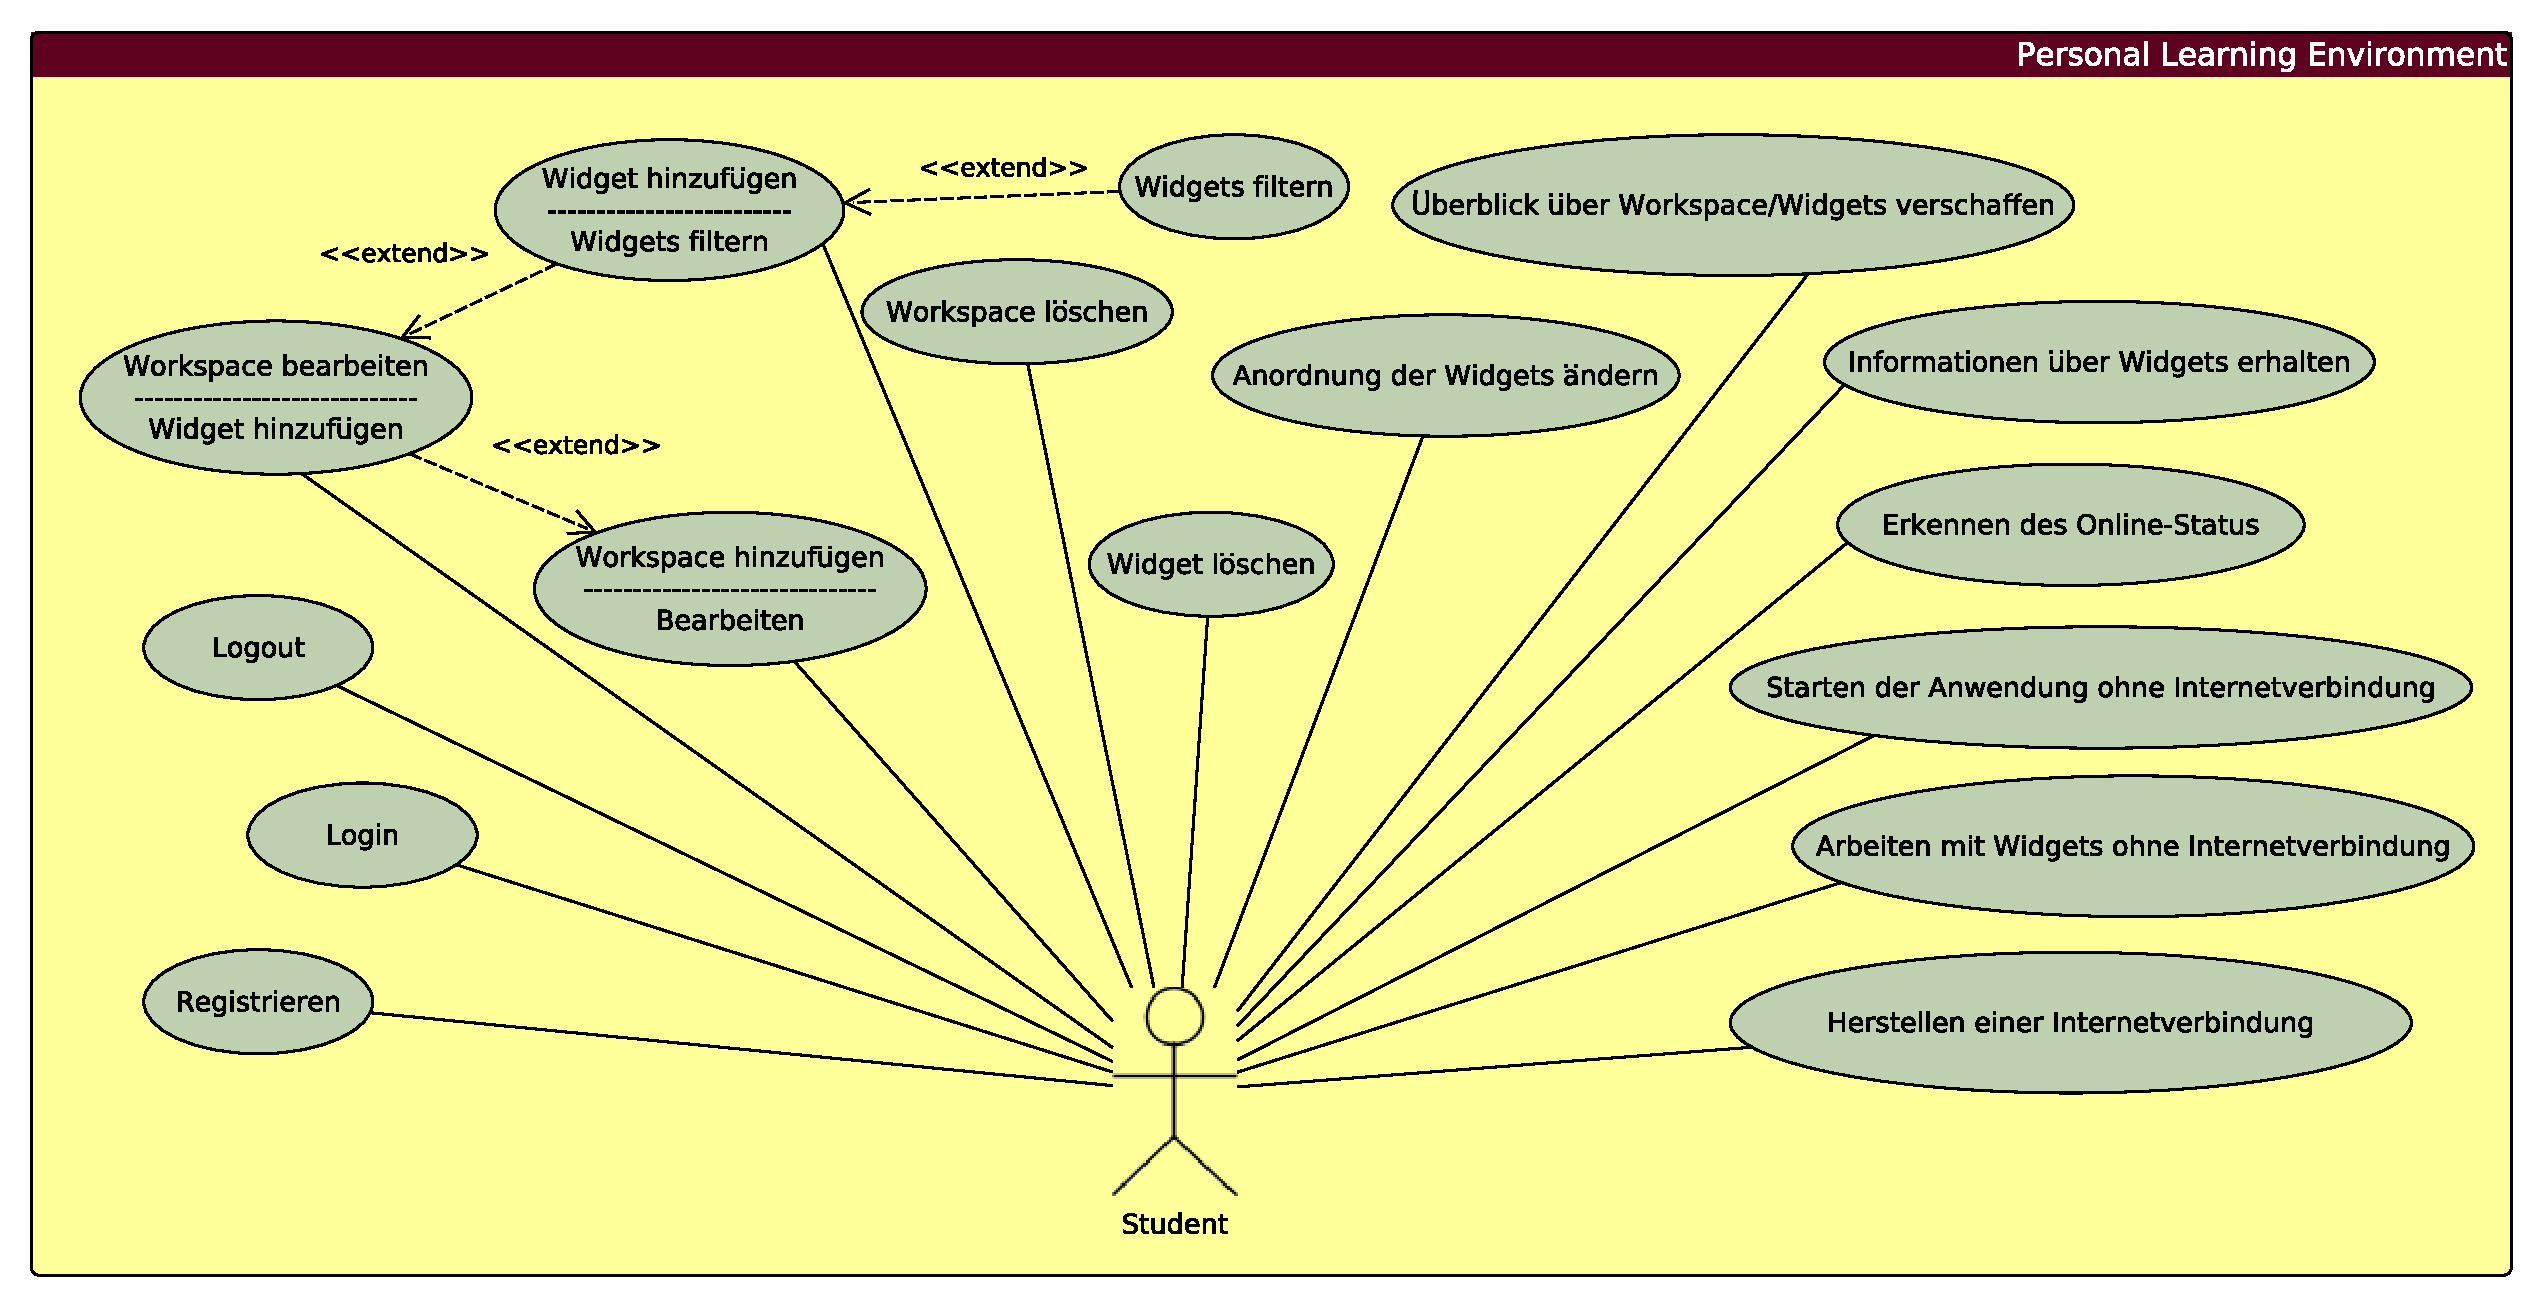
\includegraphics[width=\textwidth,height=\textheight,keepaspectratio]{./Figures/anwendungsfaelle_quer.pdf}
    \rule{35em}{0.5pt}
  \caption[Die wichtigsten Anwendungsfälle für die prototypische Personal Learning EnvironmentAnwendungsfälle der PLE]{Anwendungsfälle der PLE}
  \label{fig:anwendungsfaelle}
\end{figure}

Im folgenden werden die Anwendungsfälle aus Abbildung \ref{fig:anwendungsfaelle} in textueller Form beschrieben. Aus diesen Beschreibungen werden dann direkt die funktionalen Anforderungen an das zu entwickelnde System abgeleitet.

\subsection{Registrieren}
\textbf{use case} \emph{Registrieren}\\
\textbf{actors} Student\\
\textbf{precondition} Das System ist online, der Student ist nicht eingeloggt und es existiert mindestens ein Workspace.\\
\textbf{main flow} Der Student bekommt auf der Startseite die Möglichkeit sich für den Zugang zum System zu registrieren. Er füllt ein Formular mit seinen Daten (Vorname, Nachname, E-Mailadresse, Nutzername, Passwort) aus und schickt das Formular ab.\\
\textbf{postcondition} Der Student ist mit einer Nutzername-/Passwortkombination und seiner E-Mailadresse im System hinterlegt und kann sich somit in das System einloggen.\\
\textbf{exceptional flow} Nutzername oder Mail-Adresse bereits vorhanden. Nutzername und E-Mail-Adresse dürfen nur einmal im System vorkommen.\\
\textbf{postcondition} Der Student bekommt eine Fehlermeldung und muss seine eingetragenen Daten ändern.
 
Aus diesem Anwendungsfall folgt die funktionale Anforderung \emph{fA1}:\\
\emph{fA1: Der Anwender muss sich selbständig in dem registrieren können.}
 
\subsection{Login}
\textbf{use case} \emph{Login}\\
\textbf{actors} Student\\
\textbf{precondition} Das System ist online, der Student ist nicht eingeloggt, ist aber in dem System registriert.\\
\textbf{main flow} Der Student bekommt auf der Startseite die Möglichkeit sich im System anzumelden. Er füllt ein Formular mit seiner Nutzername-/Passwortkombination aus und schickt das Formular ab.\\
\textbf{postcondition} Der Student ist im System eingeloggt und das System präsentiert ihm eine Übersicht über seine aktuellen Workspaces und die wichtigsten aggregierten Informationen dieser.
 
Aus diesem Anwendungsfall folgen die funktionalen Anforderungungen \emph{fA2} und \emph{fA2}:\\
\emph{fA2: Der Anwender muss sich sich in das System mit Nutzername und Passwort einloggen können.}\\
\emph{fA3: Dem Anwender darf nur Zugriff auf die zu seinem Account gehörigen Workspaces und Widgets gewährt werden.}
 
 \subsection{Logout}
\textbf{use case} \emph{Logout}\\
\textbf{actors} Student\\
\textbf{precondition} Das System ist online, der Student ist eingeloggt.\\
\textbf{main flow} Der Student wählt die Aktion "`Logout"' und wird anschließend auf die Login-Seite weitergeleitet.\\
\textbf{postcondition} Die aktuelle Session des Anwenders ist beendet und es ist ohne weiteres Login nicht möglich auf die Daten des Anwenders zuzugreifen 
 
Aus diesem Anwendungsfall folgen die funktionale Anforderung \emph{fA4} und \emph{fA5}:\\
\emph{fA4: Der Anwender muss sich aus dem System ausloggen können.}\\
\emph{fA5: Nach Beendigung der Anwender-Session, darf kein Zugriff mehr auf die Daten des Anwenders bestehen.}
 
\subsection{Workspace hinzufügen}
\textbf{use case} \emph{Workspace hinzufügen}\\
\textbf{actors} Student\\
\textbf{precondition} Das System ist online, der Student ist eingeloggt.\\
\textbf{main flow} Der Student wählt die Aktion "`Workspace hinzufügen"'. Es öffnet sich hierdurch ein neuer Bereich, welcher einen neuen Workspace repräsentiert. Der Student hat nun die Möglichkeit den Workspace nach seinen Wünschen anzupasssen (extension point: Workspace bearbeiten).\\
\textbf{postcondition} Ein neuer Workspace wurde dem System des Studenten hinzugefügt.
 
Aus diesem Anwendungsfall folgt die funktionale Anforderungung \emph{fA6}:\\
\emph{fA6: Der Anwender soll neue Workspaces in seine Lernumgebung einfügen können.}\\
 
\subsection{Workspace bearbeiten}
\textbf{use case} \emph{Workspace bearbeiten}\\
\textbf{actors} Student\\
\textbf{precondition} Das System ist online, der Student ist eingeloggt und es existiert mindestens ein Workspace.\\
\textbf{main flow} Der Student wählt bei einem Workspace die Aktion "`Workspace bearbeiten"'. Der Anwender hat nun die Möglichkeit den Workspace nach seinen Wünschen zu benennen und kann Widgets zu dem Workspace hinzufügen (extension point: Widget hinzufügen).\\
\textbf{postcondition} Der Workspace wurde nach den Vorstellungen des Akteures angepasst.
 
\textbf{extend relationship}\\
\textbf{base} "`Workspace hinzufügen"'\\
\textbf{extensionPoint} Workspace bearbeiten\\
\textbf{extension} "`Workspace bearbeiten"'
 
Aus diesem Anwendungsfall folgt die funktionale Anforderungung \emph{fA7}:\\
\emph{fA7: Der Anwender soll den Namen des Workspaces ändern können.}\\
 
 \subsection{Workspace löschen}
\textbf{use case} \emph{Workspace löschen}\\
\textbf{actors} Student\\
\textbf{precondition} Das System ist online, der Student ist eingeloggt und es existiert mindestens ein Workspace.\\
\textbf{main flow} Der Student wählt bei einem Workspace die Aktion "`Workspace löschen"'. Es erscheint eine Rückfrage, welche eine Bestätigung des Löschvorganges (mitsamt aller Widgets) erfragt. Bei positiver Rückmeldung gibt das System die Nachricht des Löschens aus. \\
\textbf{postcondition} Der Workspace und alle seine Widgets sind aus dem System entfernt.
 
Aus diesem Anwendungsfall folgt die funktionale Anforderungung \emph{fA8}:\\
\emph{fA8: Der Anwender soll einen Workspace löschen können.}\\

\subsection{Widget hinzufügen}
\textbf{use case} \emph{Widget hinzufügen}\\
\textbf{actors} Student\\
\textbf{precondition} Das System ist online, der Student ist eingeloggt und es existiert mindestens ein Workspace.\\
\textbf{main flow} Der Student befindet sich in einem Workspace und wählt die Aktion "`Widget hinzufügen"' Es erscheint eine Maske in der die zur Verfügung stehenden Widgets ausgewählt werden können. Der Student wählt das gewünschte Widget und fügt es dem Workspace hinzu. Wenn gewünscht kann der Student die Liste der Widgets über Suchfilter einschränken (extension point: Widgets filtern)\\
\textbf{postcondition} Das Widget wurde dem Workspace hinzugefügt.
 
\textbf{extend relationship}\\
\textbf{base} `Workspace bearbeiten"'\\
\textbf{extensionPoint} Widget hinzufügen\\
\textbf{extension} "`Widget hinzufügen"'

Aus diesem Anwendungsfall folgt die funktionale Anforderungung \emph{fA9}:\\
\emph{fA9: Der Anwender soll über ein Auswahlfeld Widgets zu Workspaces hinzufügen können.}\\ 

\subsection{Widgets Filtern}
\textbf{use case} \emph{Widgets Filtern}\\
\textbf{actors} Student\\
\textbf{precondition} Der Student ist dabei einem Workspace ein Widget hinzuzufügen.\\
\textbf{main flow} Der Student gibt in einem Textfeld eine Zeichenkette an, nach der im Widgetnamen gesucht wird. Des weiteren kann er in einem binären Filter wählen, ob er nur Widgets angezeigt bekommen möchte, die in der Lage sind in einem Offline-Modus zu arbeiten.\\
\textbf{postcondition} In der Liste der zur Auswahl stehenden Widgets werden nur noch diejenigen angezeigt, die der Filterung entsprechen.
 
\textbf{extend relationship}\\
\textbf{base} "`Widget hinzufügen"'\\
\textbf{extensionPoint} Widgets filtern\\
\textbf{extension} "`Widgets filtern"'
 
Aus diesem Anwendungsfall folgen die funktionale Anforderung \emph{fA10} und \emph{fA11}:\\
\emph{fA10: Der Anwender muss die zur Auswahl stehenden Widgets über ein Suchfeld einschränken können.}\\
\emph{fA11: Der Anwender muss die zur Auswahl stehenden Widgets so einschränken können, dass in der Liste nur offline-fähige Widgets vorkommen.}
 
 \subsection{Widget löschen}
\textbf{use case} \emph{Widget löschen}\\
\textbf{actors} Student\\
\textbf{precondition} Das System ist online, der Student ist eingeloggt, er und es existiert mindestens ein Widget auf einem Workspace.\\
\textbf{main flow} Der Student befindet sich in einem Workspace und wählt bei einem Widget die Aktion "`Widget löschen"'. Es erscheint eine Rückfrage, welche eine Bestätigung des Löschvorganges erfragt. Bei positiver Rückmeldung gibt das System die Nachricht des Löschens aus.
\textbf{postcondition} Das Widget wurde aus dem System entfernt.
 
Aus diesem Anwendungsfall folgt die funktionale Anforderungung \emph{fA12}:\\
\emph{fA12: Der Anwender soll ein Widget löschen können.}\\
 
\subsection{Anordnung der Widgets ändern}
\textbf{use case} \emph{Anordnung der Widgets ändern}\\
\textbf{actors}Student\\
\textbf{precondition} Das System ist online, der Student ist eingeloggt und befindet sich auf der Seite eines Workspaces mit mindestens zwei Widgets.\\
\textbf{main flow} Der Student hat die Möglichkeit die einzelnen Widgets innerhalb eines Workspaces über einen Drag and Drop Mechanismus neu anzuordnen. Er wählt hierfür ein Widget mit der Maus aus und zieht es an die gewünschte Position.\\
\textbf{postcondition} Die Anordnung der Widgets innerhalb des Workspaces hat sich nach dem Wunsch des Studenten geändert.
 
Aus diesem Anwendungsfall folgt die funktionale Anforderungung \emph{fA13}:\\
\emph{fA13: Der Anwender muss in der Lage sein Widgets nach seinen Wünschen über einen Drag and Drop Mechanismus auf dem Workspace zu sortieren .}\\
 
\section{Nichtunktionale Anforderungen}\label{section:nichtfunktionale_anforderunge}
Randbedingungen, umstände etc
 
\section{Zusammenfassung}
Im den vorherigen Abschnitten wurden funktionale und nichtfunktionale Anforderungen an das zu entwickelnde System aufgestellt und beschrieben. In den folgenden zwei Tabellen sind diese Anforderungen noch einmal zusammengefasst.

\renewcommand{\arraystretch}{1.4} 
\begin{table}[h]
\caption{Funktionale Anforderungen}
\begin{tabularx}{\textwidth}{ l | X }
\emph{fA1} & \emph{Der Anwender muss sich selbständig in dem registrieren können.} \\ \hline
\emph{fA2} & \emph{Der Anwender muss sich sich in das System mit Nutzername und Passwort einloggen können.} \\ \hline
\emph{fA3} & \emph{Dem Anwender darf nur Zugriff auf die zu seinem Account gehörigen Workspaces und Widgets gewährt werden.} \\ \hline
\emph{fA4} & \emph{Der Anwender muss sich aus dem System ausloggen können.} \\ \hline
\emph{fA5} & \emph{Nach Beendigung der Anwender-Session, darf kein Zugriff mehr auf die Daten des Anwenders bestehen.} \\ \hline
\emph{fA6} & \emph{Der Anwender soll neue Workspaces in seine Lernumgebung einfügen können.} \\ \hline
\emph{fA7} & \emph{Der Anwender soll den Namen des Workspaces ändern können.} \\ \hline
\emph{fA8} & \emph{Der Anwender soll einen Workspace löschen können.} \\ \hline
\emph{fA9} & \emph{Der Anwender soll über ein Auswahlfeld Widgets zu Workspaces hinzufügen können.} \\ \hline
\emph{fA10} & \emph{Der Anwender muss die zur Auswahl stehenden Widgets über ein Suchfeld einschränken können.} \\ \hline
\emph{fA11} & \emph{Der Anwender muss die zur Auswahl stehenden Widgets so einschränken können, dass in der Liste nur offline-fähige Widgets vorkommen.} \\ \hline
\emph{fA12} & \emph{Der Anwender soll ein Widget löschen können.} \\\hline
\emph{fA13} & \emph{Der Anwender muss in der Lage sein Widgets nach seinen Wünschen über einen Drag and Drop Mechanismus auf dem Workspace zu sortieren .} \\ \hline
\end{tabularx}
\label{table:funktionale_anforderungen}
\end{table}

\section{bla}
Student 1 und Student 2 leben in Kamerun. Beide haben dort das Problem, dass der Internetzugriff aus mehreren Gründen nicht immer gegeben ist. Student 1 hat zu Hause keinen Internetzugang. Er hat nur die Möglichkeit in der Universität oder in einem Internetcafe online zu gehen. Student 2 hat einen Internetzugang, allerdings ist dieser relativ langsam und wird nach Zeit abgerechnet, so dass es vorteilhaft für ihn ist, wenn er nur für kurze Zeit online ist. Aus diesem Grund benötigen die beiden idealerweise ein System, welches ihnen die Möglichkeit bietet die neuesten Informationen auch offline zu lesen und zumindest rudimentär auch offline kleine Aufgaben zu erledigen. Diese sollten sich bei Wiederverbindung mit dem Internet mit den entsprechenden Services synchronisieren. Des Weiteren sollten sie in der Lage sein die Daten auch ohne Internetverbindung zwischen verschiedenen Rechnern auszutauschen. Insbesondere Student 1 sollte in der Lage seine Aktionen bei sich zu Hause vorzunehmen und die durchgeführten Änderungen dann an einem Rechner mit Internetanschluss zu synchronisieren. Die Anforderungen von Student 3 sind ähnlich gelagert. Er ist sehr viel unterwegs und erledigt daher viele kurze Aufgaben mit dem Smartphone. Auch hier ist eine Internetverbindung nicht immer gewährleistet ist oder sie wird temporär deaktiviert um die Akkulaufzeit zu verlängern. Durch die Arbeit an unterschiedlichen Rechnern mit potentiell unterschiedlichen Betriebssystemen, ist die Installation einer komplexen Software nicht ohne Weiteres möglich.

Idealerweise nutzen alle Studenten das selbe Basissystem und können sich hier die benötigten Services und Applikationen so zusammenstellen wie es ihren Ansprüchen entspricht.


Die Arbeit mit einer solchen Lernumgebung kann durch die folgenden Use-Cases beschrieben werden.

Das Ziel der vorliegenden Arbeit ist die Planung und Implementierung eines Prototypen für eine leichtgewichtige Personal-Learning-Environment. Die Anforderungen an das finale System lassen sich aus dem in dem nächsten Abschnitt vorgestellten Use-Case ableiten, welcher die Arbeit mit dem System verdeutlichen soll.

\section{Use Case}
Der folgende Use-Case soll durch das finale System idealerweise abgedeckt werden:

\subsection{Akteure}

\begin{itemize}
 \item Dozent mit Sitz in Hagen
 \item Student 1 mit Sitz in Kamerun (Fernuni Hagen)
 \item Student 2 mit Sitz in Kamerun (Fernuni Hagen)
 \item Student 3 mit Sitz in Berlin (Fernuni Hagen)
 \item Student 4 mit Sitz in Osnabrück (Universität Osnabrück) 
\end{itemize}

\subsection{Ausgangssituation}\label{section:ausgangssituation}
Der Dozent betreut an der Fernuni Hagen unter anderem den Kurs "`E-Learning: A new approach"'. Hierfür haben auch die Studenten 1 und 3 eingeschrieben. Für diesen Kurs hat der Dozent mehrere Kanäle zur Kommunikation angelegt. Die Studenten sollen die Kanäle wählen, die ihren Arbeitsgewohnten am meisten entsprechen. Am Ende des Semesters soll es eine Auswertung geben, welche Kanäle am häufigsten genutzt und welche von den Studenten eher ignoriert wurden. Parallel dazu werden die Systeme der Fernuni zur Online Bearbeitung der Einsendeaufgaben genutzt. Die vom Dozenten angelegten Kommunikationskanäle sind:

\begin{itemize}
 \item ein Twitter Channel
 \item eine Facebookgruppe
 \item einen eigenen Google-Calender
 \item einen Chat
 \item zur Terminabsprache und Abstimmung der nächsten Schritte soll Doodle verwendet werden
 \item ein System zur Hinterlegung von Todo-Listen
 \item einen eigenen Blog, welcher einen RSS Feed bereitstellt 
 \item Etherpad Lite soll zur gemeinsamen Erstellung von Texten genutzt werden
\end{itemize}

Die Studenten sind angehalten sich regelmäßig über Aktualisierungen der Kanäle auf dem Laufenden zu halten.

Zusätzlich haben sich Student 1, 2 und 4 zu einer virtuellen Lerngruppe zum Thema Datenbanken zusammengeschlossen. Hierfür können nicht die Systeme der Fernuni Hagen genutzt werden, da nur Student 2 momentan in dem spezifischen Kurs eingeschrieben ist. Student 1 hat sich nicht für den Kurs angemeldet und Student 4 hat überhaupt keine Möglichkeit dazu, da er nicht an der Fernuni immatrikuliert ist. Sie haben sich dazu entschlossen primär einen Chat zur Kommunikation zu benutzen.

\subsubsection{Einschränkungen/Umstände}
Student 1 und Student 2 leben in Kamerun. Beide haben dort das Problem, dass der Internetzugriff aus mehreren Gründen nicht immer gegeben ist. Student 1 hat zu Hause keinen Internetzugang. Er hat nur die Möglichkeit in der Universität oder in einem Internetcafe online zu gehen. Student 2 hat einen Internetzugang, allerdings ist dieser relativ langsam und wird nach Zeit abgerechnet, so dass es vorteilhaft für ihn ist, wenn er nur für kurze Zeit online ist. Aus diesem Grund benötigen die beiden idealerweise ein System, welches ihnen die Möglichkeit bietet die neuesten Informationen auch offline zu lesen und zumindest rudimentär auch offline kleine Aufgaben zu erledigen. Diese sollten sich bei Wiederverbindung mit dem Internet mit den entsprechenden Services synchronisieren. Des Weiteren sollten sie in der Lage sein die Daten auch ohne Internetverbindung zwischen verschiedenen Rechnern auszutauschen. Insbesondere Student 1 sollte in der Lage seine Aktionen bei sich zu Hause vorzunehmen und die durchgeführten Änderungen dann an einem Rechner mit Internetanschluss zu synchronisieren. Die Anforderungen von Student 3 sind ähnlich gelagert. Er ist sehr viel unterwegs und erledigt daher viele kurze Aufgaben mit dem Smartphone. Auch hier ist eine Internetverbindung nicht immer gewährleistet ist oder sie wird temporär deaktiviert um die Akkulaufzeit zu verlängern. Durch die Arbeit an unterschiedlichen Rechnern mit potentiell unterschiedlichen Betriebssystemen, ist die Installation einer komplexen Software nicht ohne Weiteres möglich.

Idealerweise nutzen alle Studenten das selbe Basissystem und können sich hier die benötigten Services und Applikationen so zusammenstellen wie es ihren Ansprüchen entspricht.

\subsection{Arbeitsabläufe}
Im Folgenden werden die unterschiedlichen Arbeitsabläufe mit dem System exemplarisch an Student 1 und an Student 3 dargelegt.

\subsubsection{Grundsätzlicher Arbeitsablauf für Studenten}
Um mit der PLE arbeiten zu können müssen die Studenten als erstes online eine Account in dem PLE-System erstellen. Anschließend melden sie sich mit ihren gewählten Login-Daten an. Bei erfolgreicher Anmeldung hat der Anwender die Möglichkeit direkt Workspaces zu erstellen, mit diesen zu arbeiten (Workspace umbenennen, Einstellungen vornehmen, Widgets hinzufügen etc).

\subsubsection{Arbeitsablauf Student 1}
\begin{itemize}
 \item \emph{Tag 1:} Student 1 befindet sich in der Universität und verbindet seinen USB-Stick mit einem PC. Auf diesem Stick befindet sich die ausführbare mobiler Version eines aktuellen Browsers. Er öffnet die Applikation online in diesem Browser (alle folgenden Aktionen werden mit dem selben Browser durchgeführt). Student 1 erstellt einen neuen Workspace und benennt ihn in "`PLE"' um. Anschließend sucht er die Widgets für den PLE Workspace aus der Widget-Datenbank heraus. Das System zeigt ihm dabei an, für welche Widgets eine Offline-Fähigkeit zur Verfügung steht. Daraufhin organisiert er die Anordnung der Widgets nach seinen Vorstellungen per Drag and Drop neu. Damit er mit den einzelnen Widgets auch arbeit kann meldet sich Student 1 schließlich bei den jeweiligen Services mit seinen Account-Daten an. Bevor er den Browser schließt haben sich alle Widgets mit ihren Services synchronisiert und zeigen ihm dies auch an.
 \item \emph{Tag 2:} Student 1 loggt sich an der Uni in das PLE-System ein. Das System zeigt ihm auf der Startseite (dem Dashboard) an wie viele neue Items es auf seinem PLE Workspace gibt. Ein direkter Link führt ihn zum Workspace. Er sieht, dass momentan mehrere Leute im Chat sind und unterhält sich über das Widget mit ihnen. Der Dozent hat einige globale Todos angelegt und die ersten Nachrichten kommen über den Twitter Channel herein. Nach einiger Zeit klickt Student 1 auf “jetzt offline gehen” wodurch alle Widgets seines Workspaces auf den neuesten Stand gebracht werden. Er sieht, dass Student 3 einen längeren Text im Chat geschrieben hat, beschließt diesen jedoch später zu lesen. Gleiches gilt für den Einführungsartikel des Dozenten im Kursblog. Hierfür erstellt er sich Items in seiner Todo-Liste. Abschließend schließt Student 1 den Browser und entfernt den USB-Stick.
 \item \emph{Tag 3:} Student 1 öffnet die Applikation in seinem mobilen Browser zu Hause. Das System erkennt, dass es sich im Offline-Modus befindet und versucht keine Synchronisierung mit dem Internet herzustellen. Student 1 liest den Text, den Student 3 im Chat hinterlegt hat und beantwortet die darin gestellten Fragen ebenfalls im Chatfenster. Anschließend teilt er dies über Twitter mit und erledigt sein Todo-Item.
 \item \emph{Tag 4:} Student 1 loggt sich im Internet-Cafe mit seinem mobilen Browser in das System ein. Das System erkennt, dass es online ist, lädt die neuesten Items der Services herunter und synchronisiert die nur lokal vorgenommenen Aktionen (Twitter, Chat, Todo). Per Mail hat Student 1 den Vorschlag von Student 2 bekommen gemeinsam mit Student 4 eine Lerngruppe zum Thema Datenbanken zu gründen. Hierzu wollen sie unter anderem ein Chat-System benutzen. Student 1 schlägt per Mail das ihm bekannte Chat-Widget für die PLE-Applikation vor. Er erstellt einen neuen Workspace, nennt ihn “Lerngruppe DB” und fügt das Chat-Widget mit den passenden Einstellungen hinzu.
 \item \emph{Tag 5:} Student 1 sieht in seinem Dashboard, dass es für den Workspace “Lerngruppe DB” 12 neue Items gibt. Er geht direkt zu dem Workspace und stellt fest, dass die beiden anderen Studenten sich ebenfalls in dem Chat angemeldet haben. Da momentan alle online verfügbar sind, beginnen sie ihre erste Gruppenunterhaltung und planen die weitere Vorgehensweise.
\end{itemize}

\subsubsection{Arbeitsablauf Student 3}
Student 3 nutzt das System hauptsächlich mit seinem Tablet, welches in der Lage ist sich über Wlan, sowie UMTS mit dem Internet zu verbinden.

\begin{itemize}
 \item \emph{Tag 1:} Student 3 meldet sich ähnlich wie Student 1 in der PLE an und erstellt für seine Uni-Kurse jeweils einen Workspace. Außerdem legt er sich einen Workspace an, in dem sich nicht kursspezifische Widgets finden. Hierzu gehören sein Google-Kalender, sein RSS-Reader, eine Todo Liste, sowie ein News-Widget
 \item \emph{Tag 2:} Student 3 verbindet sich zu Hause mit seinem Wlan und loggt sich in der PLE ein. Nach Prüfung des Dashboards erstellt er sich in der allgemeinen Todo Liste für den Tag. Er sieht, dass es in seinem RSS-Reader 9 neue Artikel gibt. Diese möchte er auf seinem Weg zur Uni in der U-Bahn lesen. Da dort der Empfang eher schlecht ist, synchronisiert er die PLE noch einmal. Auf dem Weg zu Uni ruft Student 3 das System auf seinem Tablet auf. Da kein Internetzugang besteht greift das System nur auf die lokalen Daten zurück. Das News-Widget in seinem globalen Workspace ist nicht offline-fähig. Aus diesem Grund wird es auch nur ausgegraut und nicht-funktional angezeigt. Der Student ist jedoch in der Lage seine lokal gecachten RSS-Artikel zu lesen. Bei Lektüre eines Artikels über Javascript fällt ihm ein, dass er sein Uni-Projekt noch mit der neuesten JQuery Version updaten wollte. Hierzu erstellt er sich ein weiteres Todo auf seiner Liste.
 In der Uni verbindet er sein Tablet mit dem Uni-Wlan. Der RSS-Reader markiert die 6 Artikel die, Student 3 in der U-Bahn gelesen hat als gelesen und synchronisiert das neueste Todo-Item mit dem Service im Internet.  
\end{itemize}

\section{Anforderungen}\label{section:anforderungen_summary}
Zusammenfassend kann also gesagt werden, dass Betreuer und Studenten stehen über unterschiedliche Kanäle in Kommunikation miteinander stehen. Es müssen Termine geplant oder auch Notizen und Nachrichten hin und hergeschickt werden. Diese Kanäle sollen auf einem zentralen Zugang so zusammengefasst sein, dass es den Teilnehmern des Kurse alle relevanten Informationen an einer aufrufen und bearbeiten zu können. Dabei sind die Teilnehmer zu unterschiedlichen Zeiten online. Die Teilnehmer sollen das System offline Nutzen können, um einfache Arbeiten wie das Schreiben von Twitter-Nachrichten, Notizen und Instant-Messaging Nachrichten oder eine Terminabsprache über einen Kalender erledigen können. Bei dem Wechsel zwischen Online und Offline müssen die Daten synchronisiert werden. Idealerweise haben die Nutzer alle Daten auf einem USB-Stick bei sich und können so von unterschiedlichsten Rechnern, wie beispielsweise in der Universität, im Internetcafe oder zu von Hause aus, arbeiten.

Daraus lassen sich mehrere Anforderungen an das zu entwickelnde System ableiten. Es soll in der Lage sein als Aggregator für die unterschiedlichsten Services und Kanäle zu dienen. Es muss möglich sein auf die wichtigsten Informationen an einem zentralen Platz zuzugreifen und diese auch zu bearbeiten (Anforderung 1). Dadurch, dass die Teilnehmer an unterschiedlichen Rechnern arbeiten, welche zum Teil nicht in ihrem persönlichen Besitz sind, ist es für sie nicht oder nur sehr schwer möglich eine neue Software zu installieren. Aus diesem Grund soll das System mit nativen Browsertechnologien ohne weitere Installation nutzbar sein (Anforderung 2). Das System muss in der Lage die wichtigsten Funktionalitäten auch dann zu Verfügung zu stellen, wenn es keinen Kontakt zu dem Internet hat (Anforderung 3). Des Weiteren soll es in der Lage sein bei einer Wiederaufnahme der Verbindung die durchgeführten Aktionen mit dem jeweiligen Service zu synchronisieren (Anforderung 4). Dies gilt insbesondere für die Arbeit mit unterschiedlichen Rechnern. Der Nutzer soll sein System an einem Computer mit dem Internet synchronisieren können und dann an einem anderen Rechner offline weiterarbeiten können. Es ist also notwendig, dass es dem Nutzer ermöglicht wird die Daten mitzunehmen (beispielsweise per USB-Stick) und an anderer Stelle weiterzuverwenden (Anforderung 5). 

Neben diesen funktionalen Anforderungen gibt es noch weitere Anforderungen, welche das System erfüllen soll. In dieser Arbeit kann nur eine prototypische Implementierung der Anforderungen erfolgen. Das System soll also als Basis für weitere Entwicklungen und Forschungsarbeiten dienen und einfach erweitert und verändert werden können (Anforderung 6). Es soll auch möglich sein auf Basis einer vorgegebenen Implementierung oder API weitere Services oder Kanäle in das System zu laden und es so beständig in seiner Funktionalität zu erweitern (Anforderung 7). Schließlich wird die Software in unterschi Bereichen, insbesondere in einem universitären Umfeld eingesetzt. Dies verlangt eine Nutzbarkeit ohne Lizengebühren für die genutzten Technologien. Daraus folgt, dass für die Umsetzun keine proprietären, sondern nur freie Technologien verwendet werden dürfen (Anforderung 8). 

\begin{table}[h]
\caption{Anforderungen}
\begin{tabular}{c || l}
1 & Informationsaggregator \\
\hline
2 & ohne Installationsaufwand lauffähig in aktuellen Browsern \\
\hline
3 & Möglichkeit des (zumindest rudimentären) Weiterarbeitens, wenn offline \\
\hline
4 & Synchronisierung der vorgenommen Änderungen, wenn wieder online \\
\hline
5 & Daten können zwischen unterschiedlichen Rechnern offline ausgetauscht werden \\
\hline
6 & kann als Basis für weitere Entwicklungen dienen\\
\hline
7 & neue Services und Kanäle sollen sich einfach in das System integrieren lassen  \\
\hline
8 & ausschließliche Verwendung freier Technologien \\
\hline
\end{tabular}
\label{table:anforderungen}
\end{table}

Die in Abschnitt \ref{section:ausgangssituation} beschriebenen Kanäle und Services müssen für eine vollständige PLE implementiert werden. Da die Umsetzung all dieser aber den Rahmen dieser Arbeit übersteigen würde und das Ziel ist einen Prototypen für die Grundlage einer solchen PLE zu schaffen, werden diese nicht in die Anforderungen aufgenommen. % Anforderungsanalyse

\chapter{Übersicht Stand der Forschung/Technik} 
\label{chapter:Kapitel4}
\lhead{Kapitel 4. \emph{Übersicht Stand der Forschung/Technik}} 

Das vorliegende Kapitel stellt Technologie und Konzepte vor, welche den Stand der Technik und Forschung im Bereich der PLE-Entwicklung darstellen oder notwendig sind, um die in Kapitel \ref{chapter:Kapitel3} entwickelnden Anforderungen an eine webbasierte und offlinefähige Personal Learning Environment zu erfüllen. Eröffnet wird das Kapitel wird mit einem Blick auf zwei unterschiedliche Konzepte zum Aufbau und zur Klassifikation von PLEs, welchem bei dem Design und der Evaluierung des Systems von Nutzen sind. Anschließend werden die aktuell verbreitetsten Widget-Frameworks beschrieben. Es folgen zwei Abschnitte zu dem technologischen Fundament, des Systems. Das Kapitel schließt mit einem Abschnitt über die Verwendung des Prototypen auf einem USB-Stick und einem kurzen Überblick über ähnliche auf dem Markt befindliche Systeme. 

\section{Konzepte zum Aufbau und zur Klassifikation von PLEs}
Das Ziel dieser Arbeit ist der Entwurf und die prototypische Implementierung einer Personal Learning Environment. Zum Erreichen dieses Zieles ist es hilfreich sich einen Rahmen zu schaffen, in dem diese Implementierung stattfinden kann. Ein solcher Rahmen kann helfen ein Vokabular zu erstellen, auf dessen Basis die benötigten Funktionalitäten der PLE  beschrieben und kategorisiert werden können. Zur Schaffung dieses Rahmens wurden für diese Arbeit zwei Konzepte gewählt, welche unterschiedliche Ansätze wählen um Funktionalitäten von PLEs auf unterschiedliche Klassen abzubilden. Zum einen gibt es den Versuch von Palmér Dimensionen zu definieren und die Funktionalitäten von PLEs diesen Dimensionen zuzuordnen. Palmér schafft damit ein System, um unterschiedliche PLE-Systeme kategorisieren zu können. Zum anderen definiert Wilson Entwurfsmuster für Personal Learning Environments. Diese Muster sollen helfen wiederkehrende Konzepte beim Entwurf einer PLE zu beschreiben und Lösungsansätze für häufig auftretende Probleme zu bieten. Diese beiden Konzepte werden im Folgenden vorgestellt. Anschließend wird unter Bezugnahme auf die Anforderungsanalyse begründet auf welchen Teilen der Schwerpunkt bei der Umsetzung dieser Arbeit liegt.

\subsection{Dimensionen nach Palmér}\label{section:dimensions_palmer} 
Palmér definiert sechs Dimensionen mit denen er so viele relevanten Funktionalitäten von PLEs wie möglich erfassen möchte (vgl. \cite{Palmer2009}). Trotz dessen sollen diese Dimensionen relativ unabhängig voneinander sein, so dass es möglich ist das unterschiedliche Plattformen einige Dimensionen mehr und andere weniger berücksichtigen und implementieren. Eine PLE kann dann Anhand des Grades ihrer Implementierung der einzelnen Dimensionen kategorisiert und bewertet werden.
\begin{enumerate}
 \item \emph{Screen-Dimension}: Die Screen-Dimension befasst sich mit Aspekten, welche die Darstellungsebene von PLEs definieren. Hierzu zählt Palmér insbesondere das User-Interface und die Usability des PLE-Containers (wie sind die Widgets angeordnet, wie können neue Widgets gesucht und hinzugefügt werden, wie einfach kann sich der Nutzer im System bewegen etc.), welcher als Einstiegspunkt in die Systembedienung dient und das User-Interface der einzelnen Widgets. Es gehören aber auch Funktionalitäten wie die Möglichkeit Inhalte und Ressourcen mit anderen Nutzern zu teilen und die Integration der selben Widgets in unterschiedlichen PLE-Containern zu der Screen-Dimension.
 \item \emph{Data-Dimension}: Mit der Data-Dimension beschreibt Palmér Funktionalitäten, die für die Portabilität der verwendeten Daten innerhalb einer PLE notwendig sind. Idealerweise sollen Widgets in der Lage sein untereinander und mit dem PLE-Container zu kommunizieren. Sie sollen Daten austauschen können und sich so weit wie möglich über ihre Zustände informieren. Des Weiteren soll es möglich sein die Daten der Widgets zu exportieren und sie an anderer Stelle oder in einem anderen PLE-Container wieder zu importieren und weiterzuverwenden. Mit der fortschreitenden Mobilität der Nutzer wird es immer wichtiger, dass der Zugriff auf die PLE auch dann möglich ist, wenn kein Zugriff auf das Internet besteht. Somit ist es nicht nur notwendig Daten zu importieren und zu exportieren, sondern auch zwischen einem Offline und einem Online-Speicher zu synchronisieren, sobald eine entsprechende Zustandsänderung eintritt.
 \item \emph{Social-Dimension}: Ein wesentlicher Bestandteil des Web 2.0 ist die Vernetzung von Freunden und Menschen mit ähnlichen Interessen untereinander. Dem trägt Palmér mit der Social-Dimension Rechnung. Diese Dimension gibt an, wie sehr eine PLE Funktionalitäten sozialer Netzwerke wie Freundeslisten integriert und Möglichkeitkeiten bietet den Zugriff auf geteilte Ressourcen auf bestimmte Typen von Freunden einzuschränken. Palmér zählt aber auch die Möglichkeit zur Erstellung von eigenen offenen oder geschlossenen Lerngruppen zu Funktionalitäten, die in diese Dimension fallen.
 \item \emph{Temporal-Dimension}: Die in der Screen- und der Social-Dimension beschriebene Kollaboration zwischen Nutzern der PLE bringt neue Anforderungen mit sich. So ist es beispielsweise notwendig oder zumindest wünschenswert, dass geänderte Inhalte sich in Echtzeit in den Instanzen der Widgets manifestieren, die ebenfalls auf diese Inhalte zugreifen. Hierbei sollten auch Probleme, wie auftretende Konflikte bei gleichzeitigem Bearbeiten der selben Ressource in Betracht gezogen werden.
 \item \emph{Activity-Dimension}: Die Activity-Dimension beschreibt die Möglichkeit Abläufe und Workflows innerhalb einer PLE aktiv zu gestalten. Hierzu gehören unterer anderem einfache Dinge wie Anleitungen als Hilfestellung für den Nutzer zur Bewegung innerhalb der PLE. Besonderen Wert legt Palmér aber auf die Abbildung von Lernsequenzen innerhalb der PLE. So können bestimmte Widgets auf bestimmte Ereignisse reagieren oder sich selbst aktivieren oder deaktivieren. Des Weiteren können unterschiedlichste Konzepte aus dem Bereich des E-Learnings wie zum Beispiel \href{http://www.imsglobal.org/learningdesign/}{IMS Learning Design}\footnote{\url{http://www.imsglobal.org/learningdesign/}} oder \href{http://ltsc.ieee.org/wg12/files/LOM_1484_12_1_v1_Final_Draft.pdf}{Learning Object Metadata (LOM)}\footnote{\url{http://ltsc.ieee.org/wg12/files/LOM_1484_12_1_v1_Final_Draft.pdf}}) in den Widgets oder dem PLE-Container selber implementiert werden.
 \item \emph{Runtime-Dimension}: Die Runtime-Dimension befasst sich mit Funktionalitäten, die die Interoperabilität zwischen PLE-Systemen und Komponenten. Nach Palmér werden Nutzer in der Zukunft nicht nur eine PLE benutzen, sondern je nach Bedürfnis oder Anwendungsfall zwischen ihnen hin und herwechseln. Hierfür sollte es möglich sein Importe und Exporte für Inhalte und Einstellungen sowohl der einzelnen Widgets als auch des PLE-Containers vorzunehmen. Damit eine Interoperabilität
 zwischen PLEs möglich wird, ist es notwendig, dass Standards geschaffen werden, welche von den unterschiedlichen PLEs anerkannt und implementiert werden. Zusätzlich gehört für Palmér auch die Möglichkeit der Einbettung und Kommunikation von PLEs in und mit größeren Systemen zu dieser Dimension.
\end{enumerate}

\subsection{Muster für das Design von Personal Learning Environments}\label{section:wilson_patterns}
\cite{Wilson2008} stellt unterschiedliche Muster vor, die bei der Entwicklung einer PLE helfen sollen. Hierbei legt er seinen Fokus auf die dezentralisierte  nutzerzentrierte Natur von PLEs. Als Motivation dafür gibt er an, dass PLEs nicht ein einfaches Stück Software seien. Vielmehr stellen sie eine Umgebung dar, in der Menschen mit Werkzeugen Ressourcen und Communities in einer lockeren und nicht vorher strikt fixierten Art und Weise kommunizieren. Dieser lockere Aufbau macht es für den Entwickler jedoch nicht leichter für den Anwender gut nutzbares System zu entwerfen. Wilson leitet seine Muster von denen ab, die von der Universität von Bolton während des "`Personal Learning Environments Reference Model Project"' Projektes entwickelt wurden. Er versucht die Anzahl der Muster jedoch von ursprünglich 77 deutlich zu reduzieren, indem er Muster, die sich auf einfache Funktionen beziehen zu größeren Gruppen zusammenfasst und so eher allgemeine Charakteristika von PLEs beschreibt.

Wilson unterscheidet zwischen zwei verschiedenen Arten von Mustern für PLEs: Muster für persönliche Anwendungen (Personal Tools) und Muster für Lernnetzwerke (Learning Networks). Personal Tools stellen hiebei die Werkzeuge dar, die ein Nutzer direkt für seine Lernaktivitäten nutzt. Er interagiert mit unterschiedlichen sozialen Netzen (zum Beispiel Lernnetzwerken) oder verwendet die Tools anderweitig für seine persönliche Art des Lernens. 
Wilson definiert Learning Networks als die Infrastruktur, welche notwendig ist um Lernnetzwerke mit Hilfer sozialer Netze oder Communities aufzubauen. Des weiteren zählt er auch die Menge der Online-Services hinzu, welche von einem Lehrinstitut den Lernenden zur Verfügung gestellt werden (vgl. \cite{Wilson2008}).

Diese Arbeit beschäftigt sich mit dem Aufbau einer PLE, welche direkt vom Nutzer für seine Lernaktivitäten verwendet wird. Learning Networks spielen hierfür keine oder eine nur sehr untergeordnete Rolle, so dass die Muster für das Erstellen eben dieser hier nicht weiter beleuchtet werden. Im Folgenden werden die Muster für Personal Tools vorgestellt. Diese ähneln meist einer Empfehlung, wie eine bestimmte Funktion umgesetzt werden sollte oder welche Funktionalitäten vorhanden sein sollten, um die Erfahrung des Nutzers im Umgang mit dem System zu verbessern.

\begin{enumerate}
 \item \emph{Discourse Monitor}\label{wilson_patterns:discourse_monitor}: In einer PLE werden Informationen aus potentiell sehr vielen und unterschiedlichen Quellen verarbeitet. Um dem Nutzer die Möglichkeit zu geben wichtige Informationen schneller herauszufiltern oder zu prioritisieren, sollte ein Discourse Monitor implementiert werden. Dieser fasst die wichtigsten Informationen aus den unterschiedlichen Quellen zusammen und bereitet sie in übersichtlicher Art und Weise auf. Dem Nutzer soll es dann möglich sein, die dargestellten Daten zu Filtern, zu prioritisieren, seine Favoriten zu kennzeichnen oder neu eingetroffene Daten einfach und zeitnah zu erkennen. 
 \item \emph{Connection Hub}: Der Nutzer einer PLE ist bei verschiedensten Netzwerken angemeldet und hat dort höchstwahrscheinlich unterschiedliche Informationen hinterlegt. Es ist auch möglich, dass eine Kommunikation über Netzwerkgrenzen hinweg stattgefunden hat. Diese Daten sind meist nicht in einem einzigen Netzwerk darstellbar. Ein Connection Hub soll in der Lage sein oder den Nutzer in die Lage versetzen diese Verbindungen darzustellen und aufzubereiten. Es wäre beispielsweise vorstellbar, dass es dem Nutzer ermöglicht wird Informationen und Daten verschiedenster Netzwerke zu kombinieren ohne, dass diese Netzwerke direkt in Kontakt zueinander stehen.
 \item \emph{Create and Mix Media}: Es ist unabdingbar, dass während des computergestützen Lernens sowohl von dem Lehrnenden, als auch von dem Lehrenden Ressourcen erstellt und diese auch anderen zur Verfügung gestellt werden. Hierzu gehören alle Arten von Ressourcen, also Textdateien, Notizen, Quellcode, Videos, Bilder, Präsentationen etc.. Die PLE sollte es dem Nutzer ermöglichen diese Ressourcen zu erstellen (auch unter Zuhilfenahme externer Services) und diese dann an unterschiedliche Netzwerke zu verteilen. 
 \item \emph{Integrate Identities}: Durch das Nutzen unterschiedlicher Services hat der Nutzer höchstwahrscheinlich auch Useraccounts bei all diesen Services erstellt. Wilson schlägt für die Vereinfachung des Umgangs mit diesen Accounts die Implementierung von Mechanismen zur Vereinfachung vor. Hierzu gehören die Nutzung von Systemen, die in der Lage sind Zugangsdaten für unterschiedliche Accounts zu verwalten und zu speichern. Es können aber auch Konzepte wie das zentrale Hinterlegen von Profildaten, zum Beispiel bei einem OpenID Server-Anbieter \footnote{\url{http://openid.net/}}, verwendet werden. Die Registrierung und der Login bei unterschiedlichen Services erfolgt dann über den Umweg eines zentralen Services, welcher alle notwendigen Daten zu dem Service übermittelt, bei dem sich der Nutzer einloggen möchte.  
 \item \emph{Manage Time and Effort}\label{wilson_patterns:manage_time_effort}: Benutzt man ein System wie eine PLE zur Organisation des persönlichen Lernens, so sollte einem dieses System Werkzeuge an die Hand geben, um das Lernen und die Arbeit zu organisieren. Hierzu gehören Zeitplaner, Kalender, Todo-Listen oder auch die Möglichkeit zur Erstellung von Notizen innerhalb des Systems.
 \item \emph{Navigation Layer}\label{wilson_patterns:navigation_layer}: Bei einer PLE hat sich der Nutzer idealerweise seine Lernumgebung aus unterschiedlichen Quellen und Werkzeugen zusammengestellt. Die Navigationsebene fasst diese in einem System zusammen und ermöglicht dem User einen einfachen Zugriff auf seine Werkzeuge. Wilson schlägt vor die Services als Widgets in der PLE einzubinden. Somit wird die PLE zu einem zentralen Zugriffspunkt oder zu einem Dashboard von dem aus der Nutzer alle seinen Aktionen ausführen kann. 
 \item \emph{Multi-platform/Multimode}\label{wilson_patterns:multimode}: Die Nutzergewohnheiten bezüglich des Gebrauchs des Internets haben sich in den letzten Jahren deutlich gewandelt \cite{VanHarmelen}. Der Zugriff erfolgt nicht mehr primär über den eigenen (Heim-)Rechner, sondern über die verschiedensten Zugriffspunkte. Hierzu gehören Computer in der Universität, am Arbeitsplatz, im Internetcafé und in letzter Zeit verstärkt auch mobile Geräte wie Smartphones oder Tablets. Aus diesem Grunde ist es notwendig, das der Zugriff auf Lernnetzwerke von all diesen Geräten aus möglich ist und die Systeme auch gut von den unterschiedlichen Geräten aus bedienbar sind. Des weiteren sollte es ein System geben, welches die Daten auf den unterschiedlichen Geräten miteinander synchronisiert, so dass der Nutzer von überall auf die aktuellsten Daten zugreifen kann.
 \item \emph{Choose, Change, Discard}\label{wilson_patterns:choose_change_discard}: Dieses Muster steht in engem Bezug zu der nutzerzentrierten Herangehensweise in dem Aufbau von PLEs. User sollen in der Lage sein, sich ihre Lernumgebung nach eigenen Vorlieben und Anforderungen einzurichten. Außerdem ist es sehr gut möglich, dass sich die Anforderungen im Laufe der Zeit ändern. Aus diesen Gründen ist es notwendig, dass es dem Nutzer frei steht Inhalte und Services innerhalb der PLE zu verschieben und anzupassen und neue Werkzeuge hinzuzufügen und nicht mehr benötigte Werkzeuge wieder zu entfernen. Die PLE sollte hierbei nicht zu viele vom Nutzer nicht änderbare Bedienungsvorgaben und Konfigurationseinstellungen machen, sondern dem Nutzer so viele Freiheiten wie möglich bei Einrichten der eigenen Lernumgebung zu geben.
\end{enumerate}

\subsection{Einordnung und Eingrenzung der Funktionalitäten der zu entwickelnden PLE}
Die funktionalen Anforderungen (siehe Tabelle \ref{table:funktionale_anforderungen}) verlangen, dass dass ein User-Interface des PLE-Containers erstellt. Dieses Interface muss so umgesetzt werden, dass es einem aktuellen Browser ohne weiteren Installationsaufwand lauffähig ist (\reqref{requirementUsageInBrowser}). Der erste Teil des Entwurfes beschäftigt sich also mit der Umsetzung der \emph{Screen-Dimension} nach Palmér. Zur Umsetzung der Anforderungen im User-Interfaces eignen sich insbesondere die von Wilson definierten \emph{Discourse Monitor}, \emph{Navigation Layer} und \emph{Choose Change and Discard} Muster. Als Einstiegspunkt in das System kann ein \emph{Discourse Monitor} dienen. Dieser fungiert als eine Startseite welche dem Nutzer die wichtigsten Informationen bezüglich seiner Widgets zur Verfügung stellt (\reqref{requirementDashboard}) und ihm durch Links die Möglichkeit gibt direkt zu den gewünschten Personal-Learning-Tools zu gelangen. Somit kann das System als ein Aggregator für unterschiedliche externe Kanäle und Services dienen (\reqref{requirementAggregator}). Der \emph{Navigation Layer} muss in einer PLE, welche als Mashup-Anwendung konzipiert wird inhärent mit eingebaut werden. Durch die Einbindung externer Widgets, wird dem Anwender nur der Funktionsumfang zur Verfügung gestellt, welche von den Widget-Entwicklern angedacht wurde. Für den vollen Funktionsumfang muss der Nutzer zum eigentlichen Service des Widgets navigieren. Die Widgets sollten dann innerhalb des Systems aggregiert und ihm in übersichtlicher Form in Form eines Dashboards präsentiert werden. Die Anforderungen \reqref{requirementWorkspaceAdd}, \reqref{requirementWorkspaceEdit}, \reqref{requirementWorkspaceDelete}, \reqref{requirementWidgetAdd}, \reqref{requirementWidgetDelete} und \reqref{requirementWidgetSortDragNDrop} verlangen, dass der Anwender Workspace und Widgets hinzugefügt, bearbeitet, entfernt und in ihrer Position verändert werden können sollten. Somit wird auch das \emph{Choose Change and Discard}-Pattern grundsätzlich im System verankert.  

Die Anforderungen \reqref{requirementOfflineWork}, \reqref{requirementOnlineSync} und \reqref{requirementOfflineStart} verlangen die Fähigkeit die wichtigsten Funktionalitäten auch offline weiterhin nutzen zu können. Wenn die Konnektivität wieder hergestellt ist sollen die Daten synchronisiert werden. Die Umsetzung dieser Anforderung beschäftigt sich also primär mit den Umgang mit Daten und Informationen und den Austausch ebendieser zwischen unterschiedlichen Systemen (zwischen dem System und den Widgets) und der Synchronisierung der Daten bei Statusänderung (von Offline- zu Online-Modus) und fallen somit in Palmérs \emph{Data-Dimension}. Die benötigte Fähigkeit des Systems zu Erkennen, ob es zu einem Zeitpunkt online oder offline ist (\reqref{requirementCheckOnlineStatus}) kann als eine Erweiterung des von Wilson vorgestellten \emph{Multimode-Patterns} betrachtet werden.   
Die restlichen Dimensionen und Muster werden im Zuge dieser Arbeit nicht implementiert, da dies über den Rahmen dieser Arbeit weit hinausgehen würde und nicht nötig ist, um die defnierten Anforderungen zu erfüllen.

\section{Widget-Frameworks}\label{section:widget_frameworks}
Damit die PLE als Aggregator für unterschiedliche Service und Kanäle verwendet werden kann, müssen diese Services als Widgets (siehe Kapitel \ref{section:widgets}) eingebunden werden. \reqref{requirementWidgetStandard} fordert, dass hierfür ein frei verfügbarer Standard genutzt wird. Um dies zu erfüllen wurden im Zuge dieser Arbeit die beiden wichtigsten frei verfügbaren Widget-Frameworks untersucht und miteinander verglichen. Im Folgenden werden diese zwei Frameworks vorgestellt. Anschließend wird eine Begründung für die Wahl eines der Framework für diese Arbeit gegeben.

\subsection{W3C Widgets}\label{section:w3c_widgets}
Die in der W3C-Recommendation spezifizierten Widgets (vgl. \cite{W3C-11-2012}) sind komplette HTML/Javascript Anwendungen, dessen gesamte Ordnerstruktur zu einer gepackten Zip-Datei zusammengefasst wird. Die Spezifikationen verlangen, dass in dieser Datei neben der Anwendung selber noch eine XML-basierte Konfigurationsdatei vorhanden ist, welche innerhalb eines widget-Wurzelelementes die Eigenschaften des Widgets definiert. Zu den Eigenschaten zählt die Widgetgröße (in Pixeln), der XML-Namespace, Icons, die in Widgetvorschauen benutzt werden sollen, externe Features, welche das Widget benötigt aber auch Informationen über den Autor oder die Lizenz unter der das Widget steht. Im Folgenden ist eine stark verkürzte Konfigurationsdatei dargestellt (aus \cite{W3C-11-2012}).
\begin{lstlisting}
<?xml version="1.0" encoding="UTF-8"?>
<widget [Attribute wie Namespace, ID etc]>
  <name short="Example 2.0">The example Widget!</name>
  <content src="myWidget.html"/>
  <license> Example license (based on MIT License) [...] </license>
</widget>
\end{lstlisting}
Über das Element $<$content$>$ wird der eigentliche Inhalt des Widgets geladen. Dieser kann also unabhängig von der späteren Verwendung innerhalb eines Widgets implementiert werden.

Neben der erwähnten Recommendation gibt es noch andere Spezifikationen rund um die Widget-Thematik, welche unterschiedliche Teilbereiche wie zum Beispiel die digitale Signierung von Widgets standardisieren\footnote{\url{http://www.w3.org/2008/webapps/wiki/WidgetSpecs}}. Als Referenzimplementierung für die W3C-Widgets fungiert das Apache-Projekt "`Wookie"'\footnote{\url{http://wookie.apache.org/}}. Wookie ist ein in Java-implementierter Widget-Container, welcher die wichtigsten Funktionalitäten für die Arbeit mit W3C-Widgets zur Verfügung stellt. Widgets, die nach dem W3C-Standard erstellt wurden, können in den Wookie Container geladen werden. Dieser übernimmt dann die Auslieferung inklusive dem benötigten Javascript-Code an die anfordernden Anwendungen. Wookie benutzt intern eine Datenbank, in der Widget-Einstellungen für jeden User oder für jede ausgelieferte Instanz eines Widgets gespeichert werden können. Mit der in den W3C-Standards spezifizierten Api können diese Einstellungen über Javascript geändert oder ausgelesen werden. Die Administration von Wookie erfolgt entweder über die Kommandozeile oder über eine REST-Api\footnote{\url{http://wookie.apache.org/docs/admin.html}} (siehe \ref{section:rest}). Für die Einbindung in andere unterschiedliche Applikationen bietet Wookie eine Connector-Api an, für welche Beispielimplementationen für Java und für PHP existieren\footnote{\url{http://wookie.apache.org/docs/embedding.html}}.

\subsection{OpenSocial Gadgets}\label{section:opensocial_gadgets}
Nach der \cite{Opensocial2013} ist OpenSocial
\begin{quotation}
  a set of APIs for building social applications that run on the web. OpenSocial's goal is to make more apps available to more users, by providing a common API that can be used in many different contexts. Developers can create applications, using standard JavaScript and HTML, that run on social websites that have implemented the OpenSocial APIs. These websites, known as OpenSocial containers, allow developers to access their social information; in return they receive a large suite of applications for their users.
\end{quotation}
OpenSocial hat sich also zum Ziel gesetzt eine allgemeine Api für die Erstellung von Social Software zu entwickeln. Hierzu definiert es allgemein Konzepte wie "`Freundeslisten"', "`Aktivitäten"' und "`Profile"' standardisiert aber auch Authentifizierungs- und Authorisierungsmechanismen. Ein wichtiger Bestandteil der OpenSocial-Api sind die OpenSocial Gadgets. Diese basieren auf den von Google entwickelten "`Google Gadgets"' \footnote{\url{https://developers.google.com/gadgets/docs/gs}} und stellen ähnlich wie die W3C-Widgets eine Api bereit, um eigenständige Webapplikationen in Mashup Anwendungen zu integrieren. Ähnlich wie für die W3C-Widgets benötigen OpenSocial Gadgets eine XML-Konfigurationsdatei. Der große Unterschied zu den W3C-Widgets liegt jedoch darin, dass sämtlicher HTML- und Javascript-Quellcode des Widgets ebenfalls in dieser XML-Datei hinterlegt wird. Der komplette Inhalt befindet sich in dem Content-Konten innerhalb der XML Datei (aus \cite{GoogleGadgetsApi2012}): 
\begin{lstlisting}
<?xml version="1.0" encoding="UTF-8" ?> 
<Module>
  <ModulePrefs title="hello world example" /> 
  <Content type="html">
     <![CDATA[ 
       Hello, world!
     ]]>
  </Content> 
</Module>
\end{lstlisting}
Eine Referenzimplementierung für die OpenSocial Gadgets ist der Apache "`Shindig"' Server\footnote{\url{http://wookie.apache.org/}}. Dieser fungiert ähnlich wie Apache Wookie als Gadget-Container und kann gerenderte Widgets an Applikationen ausliefern. Es existieren Shindig-Implementierungen in Java und in PHP.

\subsection{Wahl des Frameworks}
Für die Umsetzung in dieser Arbeit viel die Wahl auf das Framework des W3C und den Widget-Container Wookie. Somit wird der zu erstellende Prototyp in der Lage sein alle Widgets, die dem W3C-Standard entsprechen einzubinden. Die Wahl hätte auch auf die OpenSocial Gadgets und Shindig als Widget-Container fallen können. Den Auschlag für die W3C-Widgets und Wookie gaben unterschiedliche, vor allem praktikable Gründe. Das wichtigeste Argument für die Nutzung von W3C-Widgets ist, dass es möglich ist sie als ganz normale Web-Anwendungen zu entwickeln und zu testen. Es ist lediglich notwendig eine gesonderte XML-Konfigurationsdatei mit einigen Parametern zu hinterlegen. Wookie stellt dann Funktionalitäten zur Verfügung, die es erlauben aus einem einfachen Verzeichnis im Dateisystem ein nach W3C-Spezifikationen gepacktes Widget zu erstellen und dieses auch direkt in Wookie bereitzustellen. Für OpenSocial Gadgets muss der gesamte HTML- und Javascript-Quellcode innerhalb der XML-Datei liegen. Zwar gibt es auch hier Werkzeuge zur Vereinfachung der Gadget-Erstellung, aber der W3C/Wookie-Weg erschien praktikabler. Des weiteren war es zum Zeitpunkt der Entscheidungsfindung um die Dokumentation für die OpenSocial-Seite insbesondere von Shindig eher schlecht bestellt. Viele Verweise auf (z.B. auf Installationanleitungen) führten ins Leere und die PHP-Referenzimplementation war vom Entwicklungsstand ca 1,5 Jahre hinter dem Java System zurück und hatte viele nicht behobene Fehler. Dieser Zustand scheint sich jedoch zum aktuellen Zeitpunkt geändert und verbessert zu haben. Die Dokumentation von den W3C-Widgets und Wookie waren und sind relativ aktuell und existiert eine funktionierende Implementation der Connector-Api in PHP. Diese kann als Grundlage für die zu implementierende Kommunikation des Basissystems mit dem Widget-Container verwendet werden.

\section{Technologien für Offline-Web-Anwendungen}
Die Anforderungen \reqref{requirementOfflineWork}, \reqref{requirementOnlineSync}, \reqref{requirementOfflineStart} und \reqref{requirementCheckOnlineStatus} befassen sich mit den Offlinefähigkeiten des zu entwickelnden Systems. Wenn alles diese Anforderungen erfüllt sind, kann man von einer "`Offline-Web-Anwendung"' sprechen. Dieser Begriff mag sich zunächst nach einem Widerspruch in sich annhören. Normalerweise kennt der Nutzer den folgenden Arbeitsablauf, wenn er sich im Internet bewegt: Öffnen des Internetbrowser $\Rightarrow$ eingeben der gewünschten Url $\Rightarrow$ der Browser verbindet sich als Client mit dem hinter der URL stehenden Server und lädt die zur Verfügung gestellten Inhalte (Html, Javascript, Css, Medienressourcen etc) herunter $\Rightarrow$ der Browser rendert das Html/Css und führt die Anweisungen in den Javascript-Quellcode aus, so dass dem Nutzer eine funktionsfähige Seite zur Verfügung steht. Ist das System nun aber offline, kann der Browser keine Verbindung mit dem Server herstellen und erhält somit keine Daten, die er darstellen kann. Es gibt Systeme auf Html/Javascript Basis, die niemals den Kontakt mit dem Internet benötigen (vgl.\cite{Mahemoff22010}). Diese Anwendungen werden komplett aus dem Dateisystem geladen und benutzen den Browser nur für die Darstellung (z.B. \href{http://tiddlywiki.com}{TiddlyWiki}\footnote{\url{http://tiddlywiki.com/}}, ein Wiki-System, welches komplett lokal auf dem Rechner des Anwenders läuft). Diese Systeme sind aber für diese Arbeit irrelevant, da die erwähnten Anforderungen zeigen, dass für das zu entwickelnde System Anwendungen notwendig sind, die je nach Notwendigkeit sowohl online als auch offline arbeiten können. All diesen Systemen gemein ist, dass sie zumindest eine initiale Internetverbindung benötigen, bei der Zugriff auf die genutzten Ressourcen besteht.

In HTML5 gibt es im Wesentlichen zwei Mechanismen, die für die Offline-Fähigkeiten von Webanwendungen verantwortlich sind: Application-Caching und Offline-Storage (vgl. \cite{Mahemoff22010}). Der Unterschied zwischen ihnen liegt in der Art der Daten, die sie lokal vorhalten. Application-Caching ist für das Caching, also die Speicherung der zentralen Applikationslogik und des User-Interfaces im Browser zuständig. Dies bedeutet das alle benötigen Ressourcen (Html, Javascript, Css etc.) heruntergeladen und im Browsercache vorgehalten werden. Dieser Cache bleibt auch bestehen, wenn der Browser geschlossen wird. Letzteres gilt ebenso für den Offline-Storage. Offline-Storage ist ein Mechanismus, welche in der Lage ist die Daten, die der Nutzer eingibt oder bearbeitet ebenfalls im Browser zu speichern und wieder zur Verfügung zu stellen. Gemeinsam mit einem Mechanismus, der es Browsern erlaubt zu erkennen, ob sie online oder offline sind, versetzen Application-Caching und Offline-Storage den Entwickler also in die Lage ein System zu entwickeln, welches in der Lage ist ohne Konnektivität mit dem Internet erneut aufgerufen zu werden. Der Anwender kann mit dem System anschließend arbeiten, als wenn eine Internetverbindung zur Verfügung steht.

Im Folgenden werden die Möglichkeiten die HTML5 für die Umsetzung des Application-Cachings und des Offline-Storages bietet genauer beschrieben.

\subsection{Application-Caching}\label{section:appcache}
Die Basis des Application-Cachings ist eine Manifest Datei (vgl. \cite{Bidelman2010}). In dieser Datei wird hinterlegt, welche Ressourcen vom Webbrowser zwischengespeichert werden sollen. Die Datei ist eine einfache Textdatei, dessen Dateiendung frei gewählt werden kann. Es wird aber empfohlen die Manifestdatei auf .appcache enden zu lassen (vgl. \cite{W3C2012}). Wichtig ist, dass die Datei vom Webserver mit dem MIME type \texttt{text/cache-manifest} ausgeliefert wird. Dies kann z.B. für den  Apache Webserver mit dem folgenden Eintrag in einer .htaccess Datei geschehen:
\begin{lstlisting}
AddType text/cache-manifest .appcache
<IfModule mod_expires.c>
  ExpiresActive On
  ExpiresByType text/cache-manifest "access plus 0 seconds"
</IfModule>
\end{lstlisting}
Der Bereich in dem \texttt{IfModule}-Tag ist dafür zuständig, dass die Manifest-Datei selber nicht gecached wird. Dies ist momentan noch für den Firefox-Browser notwendig.

Jede HTML-Seite die den Application-Cache nutzen soll, muss diese Datei über das \texttt{manifest}-Attribut in ihrem html-Tag einbinden (vgl. \cite{html5upandrunningchapter8}). Es ist dabei egal, ob die Datei über einen relativen oder einen absoluten Pfad eingebunden wird. Sie muss nur von der HTML-Seite aus erreichbar sein:
\begin{lstlisting}
<!DOCTYPE html>
<html manifest="cache.appcache">
<body>
\end{lstlisting}

Das folgende Listing zeigt den beispielhaften Aufbau einer Manifestdatei und stammt bis auf den Fallback Bereich aus der entwickelten PLE:
\begin{lstlisting}
CACHE MANIFEST
#Rev 9
CACHE:
#Partials
/partials/dashboard
#CSS
/css/compiled/plesynd/main.css
#JS
/js/compiled/plesynd/main.js
NETWORK:
*
FALLBACK:
/ /offline.html
\end{lstlisting}

\cite{W3C2012}, \cite{html5upandrunningchapter8} und \cite{Bidelman2010} beschreiben den Aufbau der Datei folgendermaßen: Die Datei beginnt mit einem \texttt{CACHE MANIFEST}-Header, der angibt, dass es sich um eine Manifestdatei handelt. Es folgt eine Kommentarzeile mit einer Revisionsnummer. Diese Zeile ist nach der Spezifikation eigentlich nicht notwendig. Der Grund für ihr Vorhandensein ist der, dass ein Browser den Inhalt des Caches nur aktualisiert, wenn sich die Manifestdatei selber ändert, nicht aber wenn sich die Dateien, die im Manifest referenziert werden aktualisiert wurden. Ändert man nun beispielsweise eine Javascript-Datei, so würde der Browser diese Änderung nicht registrieren. Man muss zusätzlich die Manifestdatei (und sei es nur in einem Zeichen, wie hier die Revisionsnummer) ändern. Der Browser bemerkt dies und aktualisiert sowohl die Datei, als auch die von ihr referenzierten Inhalte. Die Zeilen nach dem \texttt{CACHE}-Eintrag geben die Ressourcen, an die explizit vom Browser gecached werden sollen. Wie man sieht können hier alle möglichen Ressourcentypen, also auch Binärdateien wie Bilder angegeben werden. Die Zeilen die mit einem Hash anfangen, sind nur Kommentare zur besseren Lesbarkeit. Der \texttt{NETWORK}-Eintrag defniniert eine Whitelist, welche angibt welche Ressourcen in jedem Fall über das Netz geholt werden, (auch wenn der Browser offline ist). Hier könnte beispielsweise der Zugriff auf vom Server dynamisch interpretierte PHP oder CGI Dateien definiert werden. Der in diesem Fall verwendete Platzhalter gibt an, dass alle Dateien, die nicht in der \texttt{CACHE}-Sektion definiert wurden über das Netz geholt werden. Der \texttt{FALLBACK}-Bereich beschreibt eine alternative Datei, welche angezeigt wird, wenn die angeforderte Ressource nicht im Cache liegt und kein Internetzugang besteht. Im vorliegenden Fall trifft \texttt{/} auf jede Seite ab dem Wurzelverzeichnis zu. Wenn die angeforderte Seite also nicht im Cache liegt, wird die Fallback-Datei angezeigt. Abschließend ist zu bemerken, das jede HTML-Datei, die auf eine Manifestdatei verweist implizit ebenfalls gecached wird. Der Cache kann also bei einer Webseite, durch die sich der Anwender bewegt sukzessive wachsen.

Mit dem Application-Cache ist es also möglich alle Ressourcen, die für die Anwendung benötigt werden offline im Browser zwischenzuspeichern. Die Anwendung kann nach einem initialen Download der Ressourcen auch geöffnet werden, wenn der Browser keine Internetverbindung hat. Somit eignet sich diese Technologie ideal für eine Umsetzung der Anforderung \reqref{requirementOfflineStart}.

\subsection{Offline-Storage}\label{section:offline_storage}
In der Vergangenheit wurden vor allem Cookies benutzt, um die Daten eines Anwenders innerhalb des Browsers vorzuhalten (vgl. \cite{Mahemoff22010}). Cookies haben jedoch einige schwerwiegende Nachteile, die es verhindern, dass sie für ein wirkliches Speichern von Daten und Einstellungen des Nutzers Verwendung finden können. Zum einen werden sie bei jedem Request an den Server gesendet, wodurch die Netzwerkverbindung verlangsamt wurde und potentiell unverschlüsselte Daten über das Netz geschickt wurden (außer bei Benutzung von SSL). Zum anderen sind sie auf eine Größe von 4 Kilobyte beschränkt, wodurch es nicht möglich ist eine nennenswerte Datenmenge zu hinterlegen (vgl. \cite{html5upandrunningchapter7}). Im Zuge der Entwicklung von HTML5 und immer größeren Applikationen, welche primär auf der Clientseite ausgeführt werden, wurden mehrere Technologien und Apis entwickelt, die für das Speichern der Daten im Browser verwendet werden können. Im Folgenden werden die wichtigesten drei hiervon, Web-Storage, Web SQL and IndexedDb, vorgestellt. Für alle drei Technologien befolgen die die Browser eine Same-Origin-Policy (für eine genauere Erklärung siehe Kapitel \ref{section:same_origin_policy}), d. h. nur Skripte der selben Quelle haben Zugriff auf den Speicher (vgl. \cite{Mahemoff2010}).

\subsubsection*{Web-Storage}
Web-Storage basiert auf benannten Schlüssel-/Wert Paaren, welche mit Hilfe von Javascript im Browser hinterlegt werden können (vgl. \cite{html5upandrunningchapter7}). Die Api hierfür wurde vom W3C mit dem folgenden Interface festgelegt (vgl. \cite{W3C2011}):
\begin{lstlisting}
interface Storage {
  readonly attribute unsigned long length;
  DOMString? key(unsigned long index);
  getter DOMString getItem(DOMString key);
  setter creator void setItem(DOMString key, DOMString value);
  deleter void removeItem(DOMString key);
  void clear();
};
\end{lstlisting}
Die Daten können also über \texttt{setItem(key, value)} gesetzt, über \texttt{getItem(key)} wieder ausgelesen und über \texttt{removeItem(key)} aus dem Web-Storage entfernt werden. Wichtig ist jedoch, dass der LocalStorage nur mit Zeichenketten arbeiten kann (vgl. \cite{W3C2011}). Möchte man numerische Daten wieder auslesen, müssen die mit \texttt{parseInt()} oder \texttt{parseFloat()} umgewandelt werden werden. Javascript-Objekte müssen in das Json Format umgewandelt werden, damit sie im Web-Storage hinterlegt werden können. Dies geht am besten über die \texttt{JSON.stringify} und \texttt{JSON.parse}-Methoden. Es existieren zwei unterschiedliche Implementierungen des Web-Storage Interfaces: Session-Storage und Local-Storage. Während der Session-Storage nach Schließen des Browsers geleert wird, bleiben die Werte die im Local-Storage hinterlegt werden auch nach dem Schließen des Browsers bestehen. Die \texttt{localStorage}- und \texttt{sessionStorage}-Objekte zum Zugriff auf den Local-Storage und Session-Storage sind in Javascript global, so dass ein Schreiben und Lesen folgendermaßen aussieht:
\begin{lstlisting}
// Session-Storage (wird bei Beenden des Browser geleert)
// schreiben
sessionStorage.setItem('key', 'value');
// lesen 
sessionStorage.getItem('key'));

// Local-Storage (persistent auch nach Beenden des Browsers)
// schreiben
localStorage.setItem('key', 'value');
// lesen
localStorage.getItem('key');
% \end{lstlisting}
Pro Origin erhält der Browser Zugriff auf zwischen 2,5 Megabyte und 10 Megabyte Speicherplatz.

Zusammenfassend ist zu sagen, dass die Vorteile des Web-Storage sind, dass er in allen aktuellen Browsern verfügbar ist und, dass der Zugriff über eine sehr einfache Api über Schlüssel-/Wertpaare möglich ist. Der Nachteil des Web-Storage begründet sich aber ebenfalls in dieser einfachen Speicherung. Alle Werte müssen in Zeichenketten umgewandelt werden. Es ist nicht möglich native Javascript-Objekte zu hinterlegen und abzufragen. Des weiteren ist keine Indizierung des Datenbestandes möglich und die Zugriffe auf den Speicher laufen nicht in Transaktionen, so dass im schlimmsten Fall Race-Conditions auftreten können. Aus diesem Grund eignet sich der Web-Storage nicht für Anwendungen, die auf ein schnelles Durchlaufen eines großen Datenbestandes und ein einfaches Auffinden einzelner Datensätze angewiesen sind.

\subsubsection*{Web SQL}
Web SQL ist oder besser war der Versuch ein relationales Datenbanksystem im Browser zu implementieren. Es ermöglicht alle Abfragen, die aus anderen relationalen Systemen bekannt sind, also Transaktionen, Joins, Counts etc. Ein Beispiel für die Syntax ist folgend aufgeführt (vgl. \cite{W3C2010}):
\begin{lstlisting}
function showDocCount(db, span) {
  db.readTransaction(function (t) {
    t.executeSql('SELECT COUNT(*) AS c FROM docids', [], function (t, r) {
      span.textContent = r.rows[0].c;
    }, function (t, e) {
      // couldn't read database
      span.textContent = '(unknown: ' + e.message + ')';
    });
  });
}
\end{lstlisting}
Es wird also die Methode \texttt{executeSql} auf ein Transaktionsobjekt ausgeführt. Diese Methode ermöglicht das Setzen eines Callbacks für den Erfolgs- und eines für den Fehlerfall. 

Alle vorhanden Implementierungen für Web SQL basieren auf SQLite{\url{http://www.sqlite.org/}}, welches seine eigene Teilmenge des SQL-92-Standards \footnote{\url{http://www.contrib.andrew.cmu.edu/~shadow/sql/sql1992.txt}} implementiert. Nach Ansicht des W3Cs und einiger Browserhersteller (insbesondere Mozilla) sollte ein Web-Standard nicht auf einer fertigen Technologie, sondern auf einer allgemeinen Spezifikation beruhen (vgl. \cite{W3C2010} und \cite{Ranganathan2010}). Da es aber in dieser Hinsicht keinen Fortschritt in der Entwicklung gab, hat das W3C folgenden Eintrag auf der Spezifikationseite von Web SQL hinterlegt (vgl. \cite{W3C2010}):
\begin{quotation}
 This document was on the W3C Recommendation track but specification work has stopped. The specification reached an impasse: all interested implementors have used the same SQL backend (Sqlite), but we need multiple independent implementations to proceed along a standardisation path.
\end{quotation} 

\subsubsection*{IndexedDb}
IndexedDb ist ein Versuch einen Standard für ein nicht relationales Datenbanksystem zum Offline-Speichern von Daten zu entwickeln. Genau so wie Web-Storage speichert IndexedDb Schlüssel-/Wertpaare (vgl. \cite{Mehta2012}). Die Unterschiede zum Web-Storage sind jedoch die, dass als Werte native Javascript Objekte in beliebiger Komplexität hinterlegt werden können und dass es möglich ist den Speicher nach bestimmten Attributen innerhalb der Objekte zu indizieren. Des weiteren arbeiten alle Aktionen auf der Datenbank innerhalb von Transaktionen (vgl. \cite{MDN2011}). Das Erstellen und Wiedereröffnen einer Datenbank wird hier nicht weiter beschrieben. Im Folgenden wird nur kurz gezeigt, wie ein Datenspeicher erstellt wird, ein Index auf dem Speicher gesetzt und Daten mit Hilfe dieses Indexes ausgelesen werden (analog zu \cite{Mahemoff2010}):
\begin{lstlisting}
var dataStore = db.createObjectStore("data", { keyPath: "identifier" });
dataStore.createIndex("nameIndex", "name", { unique: false });
var data = { 'identifier' : 3, 'name' : 'Roman'}
var store = db.transaction(["database_name"], 'readwrite').objectStore("data");
var request = store.put(data);
request.onsuccess(function() {...});
\end{lstlisting}  
Es wird ein Objektspeicher mit dem Namen \texttt{dataStore} erstellt. Der Speicher hat einen Primärschlüssel \texttt{identifier}. Nach diesem Property werden die Objekte im Speicher geordnet. Anschließend wird ein Index mit dem Namen \texttt{nameIndex} auf das Property \texttt{name} angelegt. Zum Schreiben der Daten wird eine Transaktion gestartet und das Objekt wird in den Speicher gelegt. Jede Aktion läuft in einem "`Request"', so dass es möglich ist \texttt{onsuccess} und \texttt{onerror} Callbacks zu definieren. Möchte man die Daten wieder auslesen, ist es möglich einen Cursor zu erstellen und alle Daten sequentiell zu durchlaufen. Die Indizes erlauben einem aber auch den direkten Zugriff auf bestimmte Daten, wenn nötig auch über einen Cursor.  Beispielweise ist es folgendermaßen möglich alle Daten mit dem Namen "`Roman"' zu finden, wenn auf diesem Property ein Index liegt (vgl. \cite{MDN2011}):
\begin{lstlisting}
var index = dataStore.index("nameIndex");
var singleKeyRange = IDBKeyRange.only("Roman");
index.openCursor(singleKeyRange).onsuccess = function(event) {
  var cursor = event.target.result;
  if (cursor) {
    // arbeite mit den Ergebnissen
    ...
\end{lstlisting} 

\subsubsection*{Zusammenfassung - Wahl der Technologie}
\begin{figure}[ht]
  \centering
  \includegraphics[width=\textwidth,height=\textheight,keepaspectratio]{./Figures/storage_browser_compatibility.pdf}
    \rule{35em}{0.5pt}
  \caption[Storage Browser Kompatibilität]{Browser-Kompatibilität der unterschiedlichen Storage-Technologien}
  \label{fig:storage_browser_compatibility}
\end{figure}
Abbildung \ref{fig:storage_browser_compatibility} zeigt, welche der vorgestellten Techologien aktuell in welchen Browsern unterstützt werden. Wie man sieht, wird bisher nur der Web-Storage flächendeckend und insbesondere auch in mobilen Browsern unterstützt. Vor allem Mozilla hat sich sehr stark gegen Web SQL und für die Verwendung von IndexedDb ausgesprochen und unterstützt auch nur noch die letztere Technologie. Gegen diese Entscheidung gibt es aufgrund der im Gegensatz zu Web SQL bedeutend komplexeren Api und der komplizierten Systementwicklung auf Basis von IndexedDb eine Menge Widerspruch (vgl. \cite{Ranganathan2010}). Momentan sieht es aber danach aus, dass ob IndexedDb zu einer W3C-Recommendation wird, während Web SQL nur von einzelnen Browserherstellern unterstützt wird.

Anforderung \reqref{requirementOfflineWork} fordert, dass der Anwender zumindest rudimentär mit dem System arbeiten kann, auch wenn keine Verbindung zu dem Backend besteht. Hierfür ist es notwendig, dass vom Anwender erstellte Daten und Änderungen im Browser vorgehalten werden, damit sie bei einer Wiederherstellung der Konnektivität synchronisiert werden können. Für die Umsetzung dieser Anforderung wurde in dieser Arbeit eine Entscheidung für den Web-Storage und gegen Web-SQL und die IndexedDb-API getroffen. Ein Grund dafür ist, dass der Web-Storage, wie in Abbildung \ref{fig:storage_browser_compatibility} deutlich wird, momentan die größte Verbreitung in aktuellen und insbesondere mobilen Browsern genießt. Insbesondere für Web-SQL ist hier in Zukunft auch keine Verbesserung zu erwarten. Des weiteren ist die Erstellung einer Applikation auf IndexedDb- und Web-SQL-Basis deutlich komplexer als auf Basis von Web-Storage, welcher für das einfache Hinterlegen von zu synchronisierenden Daten ausreicht. Durch seine einfachen Schlüssel-/Wertpaare ist er in der Umsetzung und Pflege bedeutet einfacher zu Handhaben als die anderen beiden Systeme. In Bezug auf IndexedDb ist es außerdem problematisch, dass sich die API noch nicht in einem finalisiertem Zustand befindet und noch größere Änderungen mit neuen Browserversionen zu erwarten sind.

\subsection{Online-/Offline-Erkennung}\label{section:online_offline_erkennung}
Anforderung \reqref{requirementCheckOnlineStatus} fordert, dass das System seinen Onlinestatus kennen und bemerken muss, wenn sich dieser ändert. In aktuellen Browsern existiert eine API, die es dem System erlaubt zu erkennen, ob eine Verbindung mit dem Internet besteht oder nicht. Zum einen gibt es die Eigenschaft \texttt{onLine} des globalen \texttt{navigator}-Objektes. \texttt{navigator.onLine} gibt true, wenn eine Netzwerkverbindung besteht und ansonsten \texttt{false}. Zum anderen wird bei Änderung des Online-/Offline-Zustandes ein Event aus gelöst, für welches im Code Listener definiert werden können:
\begin{lstlisting}
document.body.addEventListener("online", function () {...} 
document.body.addEventListener("offline", function () {...}.
\end{lstlisting}          
Diese in den Listenern definierten Callbacks werden bei einem Wechsel von online zu offline oder umgekehrt ausgeführt. Es ist jedoch zu beachten, dass unterschiedliche Browserhersteller "`offline"' unterschiedlich definieren. Aktuell wechselt zum Beispiel Chrome bei Verlust der Internetverbindung in den Offline-Modus, im Firefox muss dieser Modus explizit vom User angeschaltet werden (vgl. \cite{MozBug2011}).

\section{Kommunikation in Mashup-Anwendungen}
Die Anforderungen \reqref{requirementAggregator} und \reqref{requirementUsageInBrowser} verlangen, dass das System einen Aggregator, also eine Mashup-Anwendung (siehe \ref{section:mashup_anwendungen}) darstellt, der unterschiedliche Systeme in aktuellen Browsern zusammenfasst. Des weiteren soll der Nutzer in einer Art Dashboard Informationen über den Zustand der einzelnen Widgets erhalten (\reqref{requirementDashboard}). Dies erfordert, dass die Widgets in der Lage sind mit der Hauptapplikation zu kommunizieren. Die Widgets selber werden wie in Abschnitt \ref{section:widget_frameworks} beschrieben von einer Wookie-Instanz, also von einem anderen Server als die Hauptapplikation ausgeliefert. Zusammengenommen zieht dies Probleme mit Sicherheitsrichtlinien innerhalb der Browser nach sich. Dieses Kapitel behandelt diese sogenannte Same-Origin-Policy und stellt Lösungswege vor, wie trotz der gegebenen Einschränkungen eine Mashup-Anwendung funktionieren kann.

In einer Mashup-Anwendung müssen mehrere System miteinander kommunizieren. Auch und insbesondere im Hinblick auf eine einfache Erweiterbarkeit (Anforderung \reqref{requirementExtensibility}) ist es von Vorteil, wenn die Bestandteile der Anwendung für ihre Anfragen einen ähnliches Prinzip verwenden. Bei der Verwendung eines gemeinsamen Interfaces würde sich die Interoperabilität zwischen den Teilanwendungen erhöhen Entwicklern das Hinzufügen neuer Anwendungen zu der Anwendung beträchtlich erleichtern. In den letzten Jahren ist hierfür das REST-Prinzip immer weiter in den Fokus gerückt, welches ebenfalls in diesem Kapitel vorgestellt wird.

\subsection{Same-Origin-Policy}\label{section:same_origin_policy}
Moderne Browser benutzen als Teil ihres Sicherheitskonzeptes die Same-Origin-Policy. Diese bewirkt, dass Sprachen, die auf Clientseite ausgeführt werden (wie Javascript), nicht die Möglichkeit haben, Requests, also Anfragen, an einen anderen Zielpunkt als ihrem Ursprung zu starten (vgl. \cite{Ruderman2008}). Diese Policy wird also lediglich bei Zugriff auf URLs mit der selben Domain und dem selben Port, wie die URL von der die Seite geladen wurde, erfüllt. Das bedeutet, dass ein Skript auf \path{http://sop.example.com/directory1} Requests an \path{http://sop.example.com/directory2} starten kann, nicht jedoch an \path{http://example.com/directory2} (unterschiedliche Domain) oder an \texttt{http://sop.example.com:8080/directory2} (unterschiedlicher Port). Ausgenommen ist hierbei das in eine Seite eingebettete Laden von Resourcen. Hierzu gehören externe Inhalte, die über iFrames geladen werden aber auch externe Javascript-Dateien (über $<$script$>$...$<$/script$>$ Tags) und Medienresourcen wie Bilder und Videos. Des Weiteren ist es auch möglich Formulare an andere Zielpunkte als den Ursprung abzuschicken. Diese Einschränkung hat also primär Auswirkungen auf das Absenden von XMLHttp-Requests, also auf normale Ajax-Requests.

Die Same-Origin-Policy ist sehr sinnvoll um beispielsweise gefährlichem Javascript-Code das Ausspähen privater Daten zu verhindern. Sie erschwert jedoch die Entwicklung moderner Ajax-Anwendungen und insbesondere die Entwicklung von Mashup-Applikationen wie PLEs, welche prinzipiell so aufgebaut sind, dass sie ihre Inhalte und Ressourcen aus unterschiedlichen Quellen beziehen. In einer PLE wie in dieser Arbeit beschrieben werden die Widgets von einem Widget-Container wie Wookie (siehe \ref{section:widget_frameworks}) ausgeliefert und besitzen dadurch auch die Domain des Widget Containers als Origin. Arbeiten diese Widgets nun aber nicht nur lokal beim Client, sondern benötigen für ihre Funktionalität auch externe Server, so müssen sie in der Lage sein XMLHttpRequests an diese zu senden. Aus diesem Grund wurde der Mechanismus des Cross-Origin Resource Sharing (CORS) (vgl. \cite{vanKesteren2012}) eingeführt. Dieser erlaubt es unter bestimmten Bedingungen und Einschränkungen die Same-Origin-Policy zum umgehen.

\subsubsection*{CORS}
Wenn Cross-Origin Resource Sharing benutzt wird, können auf dem Server Informationen hinterlegt werden, von welchen anderen Origins er Anfragen erlaubt und welche Header in diesen Anfragen vorkommen dürfen. Ein einfacher CORS-Request vom Client zum Server sieht wie folgt aus (Workflow analog zu \cite{Hossain2012}):
Der Client sendet eine Cross-Origin-Anfrage mit einem Origin Header an den Server:
\begin{lstlisting}
GET /cors HTTP/1.1
Origin: http://api.bob.com
Host: api.alice.com
Accept-Language: en-US
Connection: keep-alive
User-Agent: Mozilla/5.0...
\end{lstlisting}
Anschließend antwortet der Server mit:
\begin{lstlisting}
Access-Control-Allow-Origin: http://api.bob.com
Access-Control-Allow-Credentials: true
Access-Control-Expose-Headers: FooBar
Content-Type: text/html; charset=utf-8
\end{lstlisting}
Alle für den CORS-Request relevanten Header beginnen mit Access-Control. \texttt{Access\allowbreak -Control\allowbreak -Allow\allowbreak -Origin} bedeutet, dass der Server eine Cross-Origin-Anfrage von dem angegebenen Origin erlaubt, \texttt{Access\allowbreak -Control\allowbreak -Allow\allowbreak -Credentials: true} besagt, dass in diesem Request auch Cookies erlaubt sind. Möchte der Client Zugriff auf Nicht-Standard-Header aus der Antwort des Servers, müssen diese in \texttt{Access\allowbreak -Control\allowbreak -Expose\allowbreak -Headers} angegeben werden.

Sollte der Client einen Request mit einer anderen Methode als \texttt{GET} oder \texttt{POST} (siehe \ref{section:rest}) senden, reicht dieser einfache Workflow nicht aus. In diesem Fall muss vor der eigentlichen Anfrage ein so genannter "`Preflight-Request"' ablaufen, welcher verifiziert, dass der Server diese Methode als CORS-Request erlaubt.

Diese Methodik erlaubt also, das Widgets von einem Widget-Container ausgeliefert werden, dadurch einen anderen Origin bekommen und trotzdem Requests an ihr eigentliches Backend senden zu können. Damit ist sie ein essentieller Baustein für den Aufbau von Mashup-Anwendungen im Internet.

\subsubsection*{Postmessage}
Für die in Anforderung \reqref{requirementWidgetInformSystem} geforderte Darstellung der wichtigsten Informationen über den Zustand eines Widgets ist es notwendig, dass die Hauptapplikation Daten von den Widgets erhalten oder auslesen kann. Mashup-Anwendungen im Internet werden wie in Kapitel \ref{section:widgets} beschrieben hauptsächlich über iframes umgesetzt. Die Same-Origin-Policy aktueller Browser erlaubt aber nur, dass die Hauptanwendung nur Daten aus iframes mit der gleichen Origin ausliest. Dies erschwert den Informationsaustausch zwischen der Hauptapplikation und den Widgets beträchtlich. Aus diesem Grund wurde das "`Postmessage"'-System entwickelt, welches diese Einschränkung auf eine sichere Art und Weise umgeht. Mit Hilfe von Postmessage ist es möglich, dass sich unterschiedliche Fenster (zum Beispiel Frames) Nachrichten schicken können. Andere Fenster können Event-Listener implementieren, welche auf diese Nachrichten hören (vgl. \cite{MDN2012}). Im folgenden Listung sieht man, wie solche eine Nachricht versendet wird (aus \cite{MDN2012}):
\begin{lstlisting}
otherWindow.postMessage(message, targetOrigin);
\end{lstlisting}
\texttt{otherWindow} ist hierbei eine Referenz auf ein anderes Fenster oder einen anderen Frame, welches über Standard-DOM-Methoden zu erreichen ist. \texttt{message} ist die Nachricht selber (kann auch ein Javascript-Objekt sein) und \texttt{targetOrigin}, ist die Origin, die \texttt{otherWindow} haben muss, damit die Nachricht verschickt wird. Damit \texttt{otherWindow} die Nachricht empfängt, muss auf dieser Seite ein Event Listener implementiert werden:
\begin{lstlisting}
window.addEventListener("message", receiveMessage);
function receiveMessage(event) {
  if (event.origin !== "http://example.org:8080")
    return;
  // ...
\end{lstlisting}
Empfängt das Fenster also eine Nachricht ist es möglich auch den Origin des Senders zu prüfen, damit man nur Nachrichten aus vertrauenswürdigen Quellen bearbeitet.

Mit dieser Technik ist es möglich, dass sich Widgets bei der Hauptapplikation registrieren und ihr Informationen, z.B. über die Anzahl der vorhandenen Items, zukommen lassen. Diese Informationen kann die Hauptapplikation dann für den Anwender aufbereiten und darstellen, so dass sich Anforderung \reqref{requirementWidgetInformSystem} erfüllen lässt.

\subsection{REST}\label{section:rest}
REST (Representational State Transfer Protocol), ist ein Architekturstil, welcher versucht 
\begin{quotation}
für statische Inhalte und dynamisch berechnete Informationen, die ein globales, gigantisches Informationssystem bilden, ein einheitliches Konzept zu definieren. (vgl. \cite{tilkovrestchapter2})
\end{quotation}
Systeme, die nach diesem Konzept entwickelt wurden befolgen die im folgenden oberflächlich beschriebenen Prinzipien. Dies führt im Idealfall zu positiven Eigenschaften, wie der losen Kopplung von Systemen, dem Vorhandensein allgemeiner Interfaces und einer dadurch erhöhten Interoperabilität, Wiederverwendbarkeit und Erweiterbarkeit führt (vgl.\cite{tilkovrestchapter2}).

Theoretisch ist es möglich ein beliebiges REST-konformes Protokoll zu entwickeln und anzuwenden, normalerweise wird jedoch das im Internet dominierende HTTP-Protokoll für die Umsetzung benutzt. Der Grund hierfür ist, dass dieses Protokoll bei korrekter Anwendung die wichtigsten Anforderungen des REST-Prinzips erfüllt und schon im Hinblick auf diesen Architekturstil entworfen wurden (einer der Hauptbeteiligten am Entwurf der HTTP-Spezifikation, Roy Fielding, hat mit seiner Dissertation :"`Architectural Styles and the Design of Network-based Software Architectures"' das REST-Prinzip entwickelt). 

Nach \cite{tilkovrestchapter2} ergeben sich für REST fünf Grundprinzipien:
\begin{enumerate}
 \item\label{enumerate_rest_principles:1} Ressourcen mit eindeutiger Indentifikation
 \item\label{enumerate_rest_principles:2} Verknüpfungen Hypermedia
 \item\label{enumerate_rest_principles:3} Standardmethoden
 \item\label{enumerate_rest_principles:4} Unterschiedliche Repräsentationen
 \item\label{enumerate_rest_principles:5} Statuslose Kommunikation
\end{enumerate}

In einem REST-Entwurf wird nach Entitäten gesucht, welche auf Ressourcen abgebildet werden. Dies ähnelt einem objektorientierten Entwurf, es gibt hierbei jedoch zwei wichtige Unterschiede. Es werden den Ressourcen keine neuen Methoden oder Verben hinzugefügt, sondern es werden nur die Standardmethoden genutzt. Um trotzdem keine Einschränkung in der Mächtigkeit dieses Prinzips in Kauf nehmen zu müssen, werden mehr Ressourcen hinzugefügt, als es eigentlich Entitäten gibt. Punkt \ref{enumerate_rest_principles:5} in den obigen Forderungen bedeutet, dass der Server keinerlei Session Informationen über den User speichert. Dies hat zur Folge, dass beispielsweise der Warenkorb in einem Shop ebenfalls als Ressource angelegt werden muss. Der Vorteil von dieser Vorgehensweise ist der, dass somit z.B. auch Lesezeichen auf einen Warenkorb angelegt werden können. Zusätzlich gibt es beispielsweise noch neben den Primärressourcen, welche einzelnen Entitäten abbilden, Listenressourcen welche für die Auflistung einer Menge von Ressourcen eines bestimmten Types genutzt werden (vgl. \cite{tilkovrestchapter4}). Im Internet besteht bereits ein eindeutiges System für die öffentliche Vergabe von Ressourcen-Identifizierern: die URI(Uniform Resource Identifier, z.B. \path{http://example.com/accounts/5?paginate=1\&page=3}). URIs stellen einen allgemein verfügbaren Namensraum zur Verfügung, in dem Ressourcen identifiziert werden können. Punkt \ref{enumerate_rest_principles:4} fordert, dass Ressourcen in unterschiedlichen Repräsentationen ausgeliefert werden können. So ist es beispielsweise möglich, dass es eine maschinenlesbare Repräsentation im XML Format und eine für Menschen im Browser darstellbare Repräsentation im HTML Format gibt. Der Client kann über einen Accept-Header ein bestimmtes Format anfordern.
Möchte man zum Beispiel einen Kunden über eine Ressource abbilden könnte der Identifizerer \path{http://example.com/customers/4} sein. Eine Anfrage der Darstellung kann dann als einfacher HTTP-Request abgeschickt werden:
\begin{lstlisting}
GET /customers/4 HTTP/1.1
Host: example.com
Accept: application/xml 
\end{lstlisting}
Der Server gibt in mit einem Statuscode (hier 200 OK) zurück, ob die Anfrage erfolgreich war und fügt dann die gewünschte Repräsentation der Ressource an:.
\begin{lstlisting}
HTTP/1.1 200 OK
Content-Type: text/xml; charset=utf-8
Content-Length: ...

[XML spezifische Kopfzeilen]
<customer href="./customers/4">
  <name>Roman Sachse</name>
  <orders>
    <order>
      <delivered>true</delivered>
      <link>http://example.com/orders/54>
\end{lstlisting}
In der Antwort des Server finden sich Links auf weitere mit dem Kunden verknüpfte Ressourcen. Dies ist eine Umsetzung des Hypermedia-Prinzip, welches für ein vollkommenes REST-System fordert (vgl. \cite{tilkovrestchapter2}), dass sich Client ab einem Startpunkt aus nur durch das Verfolgen Links durch das gesamte System bewegen könnte. Eine Listenressource würde man über \path{http://example.com/customers} abfragen, die Antwort könnte dann in XML Verweise auf die einzelnen Customer erhalten. Zusätzlich könnten bei gewünschter Paginierung der Ergebnisse (beispielsweise über Query-Parameter wie \path{http://example.com/customers?page=2} noch Links auf die vorherige und nächste Seite zurückgegeben werden.

Wie man in der obigen Anfrage sieht, wird eine Anfrage mit dem Verb GET an den Server geschickt. Das HTTP-Protokoll stellt unterschiedliche Standardmethoden bereit, mit denen ein Client eine Ressource Abfrage kann. Der Vorteil bei der Nutzung dieser Standardmethoden liegt darin begründet, dass mit ihnen theoretisch ein Interface existiert, mit dem alle Ressourcen abgefragt werden können und die ein Server für alle Ressourcen versteht. Sollte dies einmal nicht der Fall sein, kann der Server mit einer Fehlermeldung im Sinne von "`Methode wird für diese Ressource nicht unterstützt"' antworten. Für Methoden gibt es zwei wichtige Merkmale. Sie können sicher und/oder idempotent sein (vgl. \cite{tilkovrestchapter5}). Sicher bedeutet in diesem Fall, dass ein Request auf eine Ressource mit dieser Methode keine Seiteneffekte hat, d.h. die Ressource nicht verändert wird. Idempotent meint, dass eine Methode auf sich selbst angewandt wieder das selbe Ergebnis liefert (mathematisch: f(x) = f(f(x))). Idempotenz ist in diesem Umfeld ein wichtiges Konzept, da es immer möglich ist, dass der Client durch unerwartete Probleme (Verbindungsabruch etc.) keine Antwort vom Server erhält auf seine Anfrage erhält. Bei idempotenten Methoden kann er seine Anfrage einfach noch einmal stellen, ohne befürchten zu müssen, dass auf dem Server, ein Zustand eintritt, den er nicht erwartet hat. Die HTTP stellt acht Methoden bereit, wobei hier nur die wichtigsten fünf kurz vorgestellt werden (vgl. \cite{tilkovrestchapter5}:
\begin{enumerate}
 \item mit \texttt{GET} fordert der Client eine Repräsentation (in einem zu spezifierendem Format) einer Ressource an. sicher: ja, idempotent: ja
 \item \texttt{PUT} weißt einen Server an eine Ressource updzudaten und wenn nicht vorhanden zu erstellen. sicher: nein, idempotent ja 
 \item \texttt{POST} weißt einen Server an eine Ressource zu erstellen (wird an Listenressource gesendet). sicher: nein, idempotent: nein
 \item \texttt{DELETE} weißt einen Server an eine Ressource zu löschen. sicher: nein, idempotent: ja
 \item \texttt{OPTIONS} liefert Metadaten für eine Ressource - z.B. Allow-Header, welche angeben, welche Methoden/Header akzeptiert werden, wichtig für CORS (siehe \ref{section:same_origin_policy})
\end{enumerate}

Um zu den Customer-Ressourcen aus dem obigen Beispiel also einen Kunden hinzuzufügen, müsste man einen POST-Request an die Listenressource \path{http.example.com/customers} senden. Ein einzelner Kunde kann mit einem GET-Request an die Primärressource \path{http.example.com/customers/4} ausgelesen werden. PUT oder DELETE würden die Ressource dementsprechend aktualisieren oder löschen

GET und POST sind die am häufigsten genutzten Methoden. Der Grund hierfür ist, dass diese beiden Methoden der normale Weg eines Brwoser sind mit einem Server zu kommunizieren. Jeder direkte Aufruf einer URI über einen Browser sendet eine GET-Anfrage an einen Server. Die im Web häufig anzutreffenden Formulare werden meist über eine POST-Anfrage abgeschickt. So werden diese beiden Methoden ausserhalb von Anwendungen, die dem REST-Prinzip folgen, auch für alle anderen Anfragen benutzt, so dass man sich bei diesen Anwendungen nicht sicher sein kann, ob ein GET-Request an eine URI nicht ein Ändern oder Löschen der Ressource zur Folge hat (man betrachte beispielsweise die URI: \path{http://example.com/customers/5?action=delete}).

Wird eine Anwendung im Hinblick auf REST-Prinzipien umgesetzt, so vereinfacht dies die Erweiterung dieses Systemes beträchtlich (Anforderung \reqref{requirementExtensibility}). Insbesondere für Mashup-Anwendungen bei denen unterschiedliche Systeme miteinander kommunizieren müssen, ist beispielsweise die Nutzung eines gemeinsamen Methodeninterfaces sehr hilfreich, da nicht für jedes System ein weiteres Kommunikationsprotokoll erstellt werden muss. Das System dieser Arbeit hat noch die zusätzliche Anforderung den Anwender in die Lage zu versetzen auch offline zu arbeiten (Anforderung \reqref{requirementOfflineWork}). Wenn das System für das Speichern der Daten im Browser ebenfalls auf REST aufsetzt, wird es mit relativ wenig Aufwand möglich sein weitere offlinefähige Widgets für unterschiedliche Services zu erstellen. Die Art des Services ist dabei egal, solange er in der Lage ist einfache REST-Anfragen zu verstehen, zu verarbeiten und standardkonform auf sie zu antworten. Für den Entwickler wird es in diesem Fall vollkommen transparent sein, ob sich das System in einem Online- oder Offline-Zustand befindet. Er kann unabhängig von dem Zustand die Daten ohne zu implementierende Fallunterscheidungen speichern und abfragen.

\section{Eine PLE auf dem USB-Stick}
Anforderung \reqref{requirementUsbStick} fordert die Möglichkeit das System auf unterschiedlichen Rechnern zu benutzen und die Daten offline zwischen diesen Rechnern auszutauschen. Da alle systemrelevanten Daten im Browser hinterlegt werden (Application-Cache (siehe \ref{section:appcache}) und Web-Storage (siehe \ref{section:offline_storage}), ist es notwendig die gesamte Browserinstallation zwischen unterschiedlichen Rechnern hin und herbewegen zu können. Der einfachste Weg hierfür ist die Installation des Browsers auf einem portablen Speichermedium wie einem USB-Stick. Hierfür gibt es beispielsweise die Open-Source-Anwendung \href{http://portableapps.com/}{PortableApps}\footnote{\url{http://portableapps.com/}}, die genau dies erlaubt wodurch diese Anforderung relativ leicht zu erfüllen ist. 

\section{Ähnliche Systeme}\label{section:aehnliche_systeme}
Wie in Kapitel \ref{chapter:Kapitel2} beschrieben gibt es zwei unterschiedliche Arten vom E-Learning Systemen. Lern-Management-Systeme (LMS) und Personal Learning Environments (PLE). Vertreter der klassischen LMS sind beispielsweise \href{https://moodle.org/}{Moodle}\footnote{\url{https://moodle.org/}} oder \href{http://www.sakaiproject.org/}{Sakai}\footnote{\url{http://www.sakaiproject.org/}}. Diese Systeme verfolgen einen sehr kurszentrierten Ansatz und werden hier nicht eingehender betrachtet, da sie nicht dem Konzept einer Personal Learning Environments entsprechen. In den Bereich der PLEs fallen Systeme, die es dem Anwender erlauben sich sein eigenes System aus Widgets zusammenzubauen, also wirklich als Informationsaggregatoren fungieren. Die zwei wichtigsten und verbreitetsten Vertreter dieser Art Anwendungen sind das von Google entwickelte \href{http://www.google.de/ig}{iGoogle}\footnote{\url{http://www.google.de/ig}} und \href{http://www.netvibes.com}{Netvibes}\footnote{\url{http://www.netvibes.com}}. Beide Systeme verfolgen den Ansatz einer personalisierbaren Homepage. Es ist möglich Widgets für die unterschiedlichsten Services aus einer Widgetdatenbank auszuwählen und dem System zuzuordnen. Die Widgets können innerhalb des Systemes unterschiedlichen frei definierbaren Arbeitsflächen sogenannten Workspaces oder Tabs zugewiesen und dort per Drag an Drop angeordnet werden. Als Widgetformat benutzt Netvibes die eigens entwickelte "`Universal Widget Api"' (\href{http://dev.netvibes.com/doc/uwa}{UWA}\footnote{\url{http://dev.netvibes.com/doc/uwa}}), welche erlaubt Widgets auf Basis von HTML, XML, und Javascript zu entwickeln. Für iGoogle hat Google die sogenannten \href{https://developers.google.com/gadgets/}{Google Gadgets}\footnote{\url{https://developers.google.com/gadgets/}} entworfen. Die in Abschnitt \ref{section:opensocial_gadgets} vorgestellten OpenSocial Gadgets basieren zum Großteil auf der Google Gadgets Spezifikation. Zusätzlich zu den eigenen Widgets werden auf der iGoogle Startseite neben einem standard Suchfeld für die Google Suche nicht entfernbare Direktlinks zu anderen Google-Services angeboten wie Calender, Google Drive oder Google+ angeboten. Weder das Netvibes noch das iGoogle Grundsystem stehen als Open Source im Quellcode zur Verfügung. Beide Systeme sind kostenlos, zusätzliche Funktionen (insbesondere für Business Anwendungen) können bei Netvibes für 499 Dollar im Monat dazugebucht werden. Google hat angekündigt das iGoogle-System zu Gunsten von des Chrome App Shops oder Google Play Marktplatzes für Android-Systeme zum 1. November 2013 abzuschalten \cite{Google2012}.

In ihrer Funktionalität und Arbeitsweise ähneln sie sehr dem in dieser Arbeit zu entwickelnden System. Beide Systeme besitzen jedoch keine expliziten Funktionalitäten zum Offline-Arbeiten. Netvibes erlaubt es einzelne Artikel zum Beispiel in einem Newsfeed als "`zum später lesen"' zu markieren und herunterzuladen. Es gibt jedoch weder Möglichkeit die Seite erneut zu laden, wenn keine Internetverbindung besteht, noch eine Möglichkeit offline Weiterzuarbeiten und vorgenommene Änderungen bei einer erneuten Verbindung zu synchronisieren. 

TODO Erweiterungen Moodle? % Übersicht Stand der Forschung
 
\chapter{Lösungsansatz} 
\label{chapter:Kapitel5}
\lhead{Kapitel 5. \emph{Lösungsansatz}}  

\section{Überblick - Plesynd}
\begin{landscape}
\begin{figure}[ht]
  \centering
  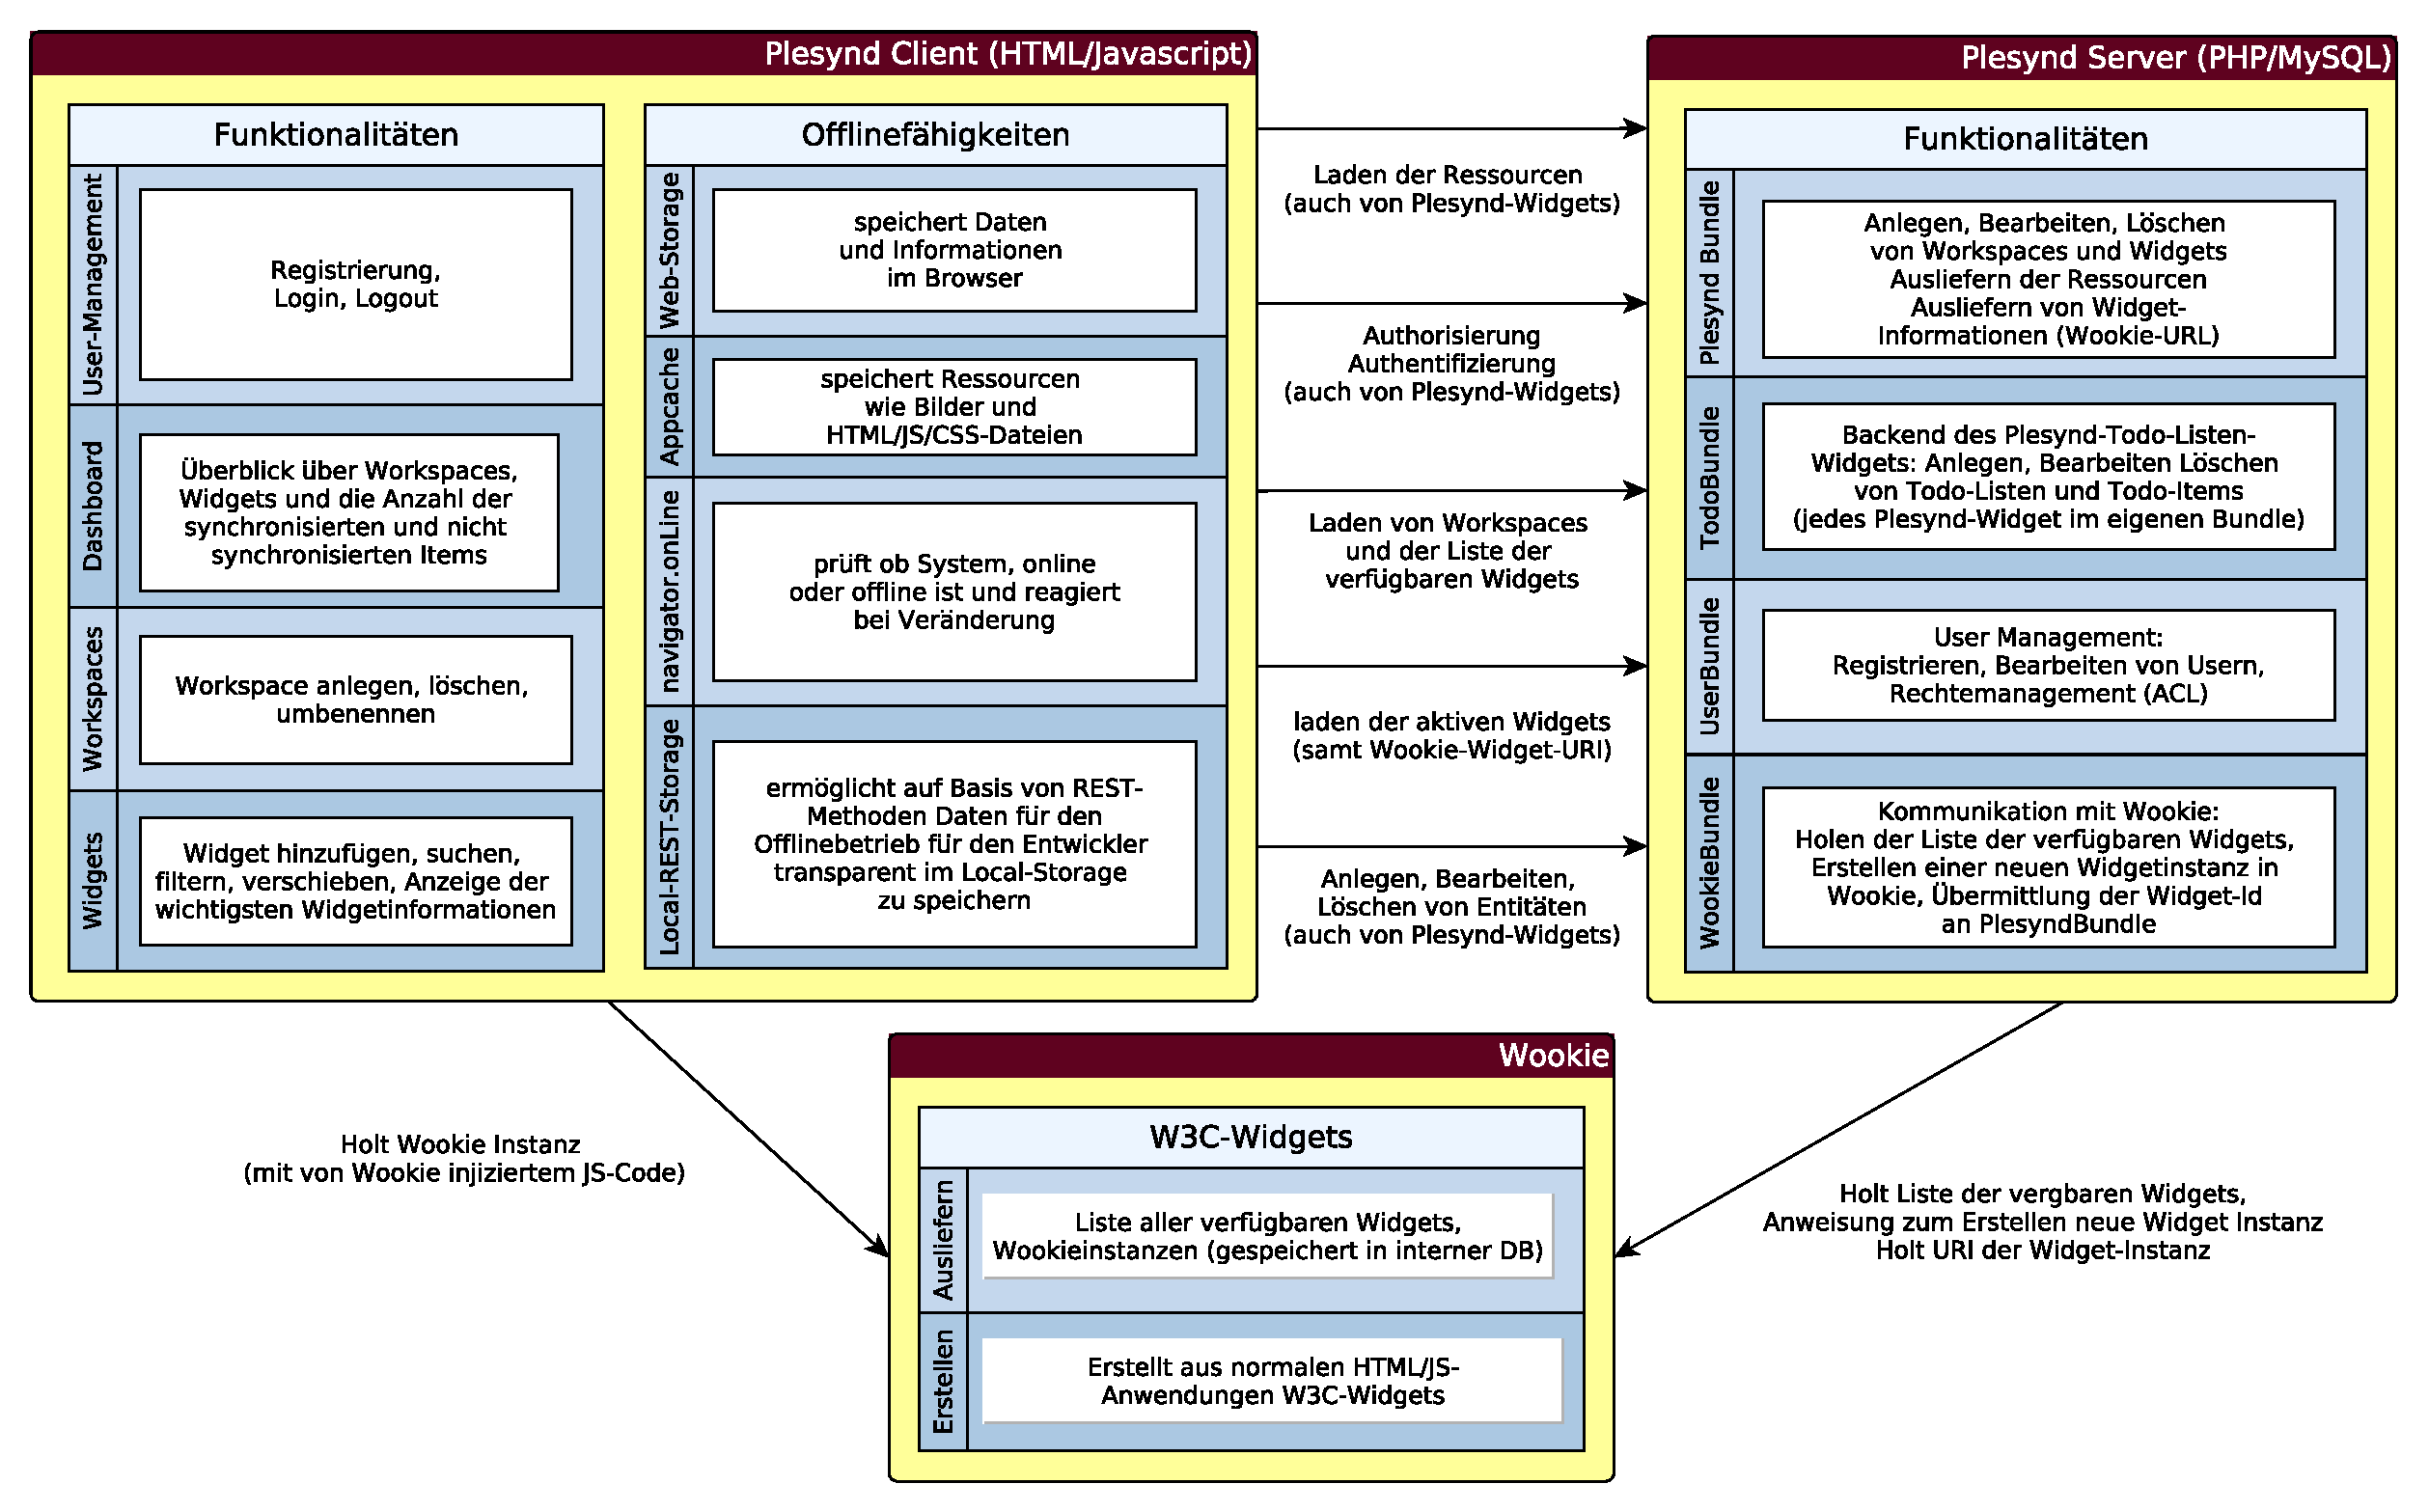
\includegraphics[height=\textheight,keepaspectratio]{./Figures/konzeptionelle_loesung_table.pdf}
    \rule{35em}{0.5pt}
  \caption[Zusammenspiel der wichtigsten Komponenten innerhalb von Plesynd]{Zusammenspiel der wichtigsten Komponenten innerhalb von Plesynd}
  \label{fig:konzeptionelle_loesung2}
\end{figure}
\end{landscape}


Das Ziel dieser Arbeit war die Entwicklung eines leichtgewichtigen Prototypen einer Personal Learning Environment, welcher die Anforderungen aus \ref{section:anforderungen_summary} erfüllt. Für die Umsetzung dieses Ansatzes wurde das Hauptaugenmerk auf die Screen- und die Data-Dimension nach Palmér zu gerichtet (siehe Abschnitt \ref{section:dimensions_palmer}). Die Screen-Dimension, also das User-Interface wird in Abschnitt \ref{section:user_interface} beschrieben. Bei der Umsetzung der Data-Dimension handelt es sich primär um die Implementierung der Online-Offline-Fähigkeit des Systems (siehe Abschnitt \ref{section:technische_umsetzung}).

Der Name des Systems lautet Plesynd (Personal-Learning-Environment Synchronize Data) und wird wie das englische "`pleasant"' (angenehm) ausgesprochen. Plesynd ist ein webbasiertes Dashboard, welches die Möglichkeit bietet mit unterschiedlichen Widgets in Kommunikation zu treten. Wichtig ist hierbei eine Abgrenzung zu zentralisierten Lern-Management-Systemen wie Moodle oder Sakai. Die sind sehr kurszentriert und können auch nur schwer mit den Wilson-Patterns für nutzerzentrierte Personal-Learning-Environment Systeme klassifiziert werden (siehe \ref{section:wilson_patterns}). Aus diesem Grund orientiert sich Plesynd viel stärker an bestehenden Widget-Aggregatoren wie iGoogle oder Netvibes (siehe \ref{section:aehnliche_systeme}). Um dem Nutzer die Möglichkeit zu geben in unterschiedlichen Kontexten mit dem System zu arbeiten und so von dem kurszentrierten Ansatz von LM-Systemen zu dem nutzerzentrierten Ansatz von PLEs zu kommen, wird das System dem Nutzer die Möglichkeit geben, seine Widgets in unterschiedliche Bereiche, sogenannte Workspaces, aufzuteilen. Die Anzahl der Workspaces ist frei und jeder Workspace kann individuell benannt werden.

Der entscheidende Unterschied von Plesynd zu den erwähnten Systemen ist die Offline-Fähigkeit der PLE. Es wurde ein Ansatz entwickelt, der es ermöglicht Widgets so zu implementieren, dass ihre Informationen offline verfügbar gemacht werden. Des weiteren kann auch auch offline mit Plesynd und den Widgets weitergearbeitet werden. Sobald wieder eine Online-Verbindung hergestellt ist, werden die veränderten Daten mit dem Backend synchronisiert.

Das Ziel beim Design von Plesynd war es dem Nutzer die Bedienung so einfach wie möglich zu machen. Die wichtigsten Informationen sollten ihm direkt direkt zur Verfügung gestellt werden (sind alle Daten aktuell, welche Widgets werden benutzt, ist das System offline oder online etc). Widgets können gesucht, nach Offline-Kompatibilität gefiltert und dem System hinzugefügt werden. Es existiert ein Dashboard, welches dem Nutzer anzeigt welche Widgets auf welchen Workspaces zur Verfügung stehen und wie ihr Online-/Offline-Status ist. 

\section{Technische Umsetzung}\label{section:technische_umsetzung}
Plesynd wurde auf der Serverseite mit PHP und auf der Clientseite mit Html5 und Javascript umgesetzt. Die verwendeten Frameworks und zusätzlichen Werkzeuge werden in Kapitel \ref{section:entwicklungsumgebungen_tools} vorgestellt und eingehender beschrieben. Für die Kommunikation mit dem Server verwendet das System REST konforme Anfragen (siehe Kapitel \ref{section:rest}). 
Die Heraustellungsmerkmale von Plesynd sind die Fähigkeit die wichtigsten Funktionalitäten auch offline weiterhin nutzen zu können und die Synchronisierung der Daten, wenn das System wieder online ist. Klassifiziert man diese Fähigkeiten wie in Kapitel \ref{section:klassifizierungsmethoden} beschrieben, so gehören sie in die von Palmér definierte Data-Dimension. Diese Funktionalitäten beschäftigen sich primär mit den Umgang mit Daten und Informationen und den Austausch ebendieser zwischen unterschiedlichen Systemen (zwischen Plesynd und den Widgets) und der Synchronisierung der Daten bei Statusänderung (von Offline- zu Online-Modus). Die Fähigkeit zum Umgang mit unterschiedlichen Status des System kann auch als eine Erweiterung des von Wilson vorgestellten Multimode-Patterns (siehe Seite \pageref{wilson_patterns:multimode}) betrachtet werden. 

Die Möglichkeit Javascript, Css und Html Dateien im Browser zu speichern wurde mit der Html5 Appcache-API umgesetzt (siehe Kapitel \ref{section:appcache}). Sollte einmal eine andere Speichertechnik als der Web-Storage benötigt werden, ist das System so implementiert, dass die Art der lokalen Speicherung losgelöst von der restlichen Anwendung umgestaltet werden kann.

Plesynd erkennt über ein globales Javascript-Event (siehe Kapitel \ref{section:online_offline_erkennung}), wenn sich der Browser in einem Zustand befindet, in dem er keine Konnektivität mit dem Internet besitzt. Das System informiert den User darüber, kann aber auch entscheiden, welche Funktionalitäten es dem Nutzer zur Verfügung stellen darf. Nimmt der Anwender Änderungen an den Daten vor, werden diese nur in den Local-Storage geschrieben. Sobald sich das System wieder mit dem Internet verbindet erkennt Plesynd diese Zustandsänderung und synchronisiert die Daten mit den zugrunde liegenden Services. 

TODO Erstellung einer Grafik mit den Komponenten und Zusammenspiel dieser


Wookie
Plesynd 
W3C

Browser, local storage 

Probleme mit der bei modernen Browser üblichen Same-Origin-Policy für Request wurden mit dem Cross-Origin Resource Sharing (CORS) Mechanismus (siehe \ref{section:same_origin_policy}) und die Postmessage-API (siehe \ref{section:same_origin_policy}) gelöst. 


\begin{lstlisting}
<preference name="plesynd_offline_compatible" value="true"/>
\end{lstlisting}

\section{User Interface}\label{section:user_interface}
Für die Umsetzung der Screen-Dimension, also des User-Interfaces kommen in Plesynd drei wichtige Konzepte zum Einsatz: Dashboard, Widgets und Workspaces. 

Über Widgets werden die unterschiedlichen Werkzeuge und Services, die ein Nutzer innerhalb des Systems nutzen möchte eingebunden (siehe: Kapitel \ref{section:widgets}). Die Umsetzung der einzelnen Widgets liegt in der Hand des jeweiligen Designers. Da Plesynd Wookie als Widget Container benutzt, ist es möglich alle W3C-Widgets in das System einzubinden. Für diese Arbeit wurde ein Todo-Listen-Service entwickelt für den als prototypische Entwicklung ein Widget mit Online-/Offline-Fähigkeiten implementiert wurde. Besitzt ein Widget Online-/Offline-Fähigkeiten so erhält es eine von Plesynd zur Verfügung gestellte Statusleiste, in der der aktuelle Online-/Offline-Status, sowie die Anzahl der verfügbaren Items und der noch nicht synchronisierten Item angezeigt wird (Abbildungen \ref{fig:plesynd_workspace_online} und \ref{fig:plesynd_workspace_offline}).
\begin{figure}
  \centering
  \includegraphics[width=\textwidth,height=\textheight,keepaspectratio]{./Figures/plesynd_workspace_online.png}
    \rule{35em}{0.5pt}
  \caption[Plesynd User-Interface: Workspace Online]{Ein Workspace mit unterschiedlichen Widgets}
  \label{fig:plesynd_workspace_online}
\end{figure}

\begin{figure}
  \centering
  \includegraphics[width=\textwidth,height=\textheight,keepaspectratio]{./Figures/plesynd_workspace_offline.png}
    \rule{35em}{0.5pt}
  \caption[Plesynd User-Interface: Workspace Offline]{Die wichtigsten Unterschiede im Offline-Modus}
  \label{fig:plesynd_workspace_offline}
\end{figure}
Der Nutzer hat die Möglichkeit Widgets nach Themen oder Einsatzgebieten zu gruppieren. Dies geschieht über sogenannte Workspaces. Workspaces sind vom Nutzer frei und in unbegrenzter Zahl hinzufügbare Bereiche im System. Sie sind über eine Reiter-Navigation zu erreichen und können jederzeit umbenannt oder auch wieder gelöscht werden (Abbildung \ref{fig:plesynd_workspace_edit}). 
\begin{figure}
  \centering
  \includegraphics[width=\textwidth,height=\textheight,keepaspectratio]{./Figures/plesynd_workspace_edit.png}
    \rule{35em}{0.5pt}
  \caption[Plesynd User-Interface: Bearbeiten von Workspaces]{Workspaces können direkt bearbeitet werden.}
  \label{fig:plesynd_workspace_edit}
\end{figure}

Jedes Widget kann einem Workspace hinzugefügt werden. Die Position der Widgets innerhalb eines Workspaces kann über einen Drag and Drop Mechanismus angepasst werden. Die Startseite stellt als Dashboard die wichtigsten Informationen dar. Jeder Workspace wird in einer eigenen Tabelle inklusive seiner Widgets und der Anzahl der zur Verfügung stehenden Widgets präsentiert. Über direkte Links innerhalb des Dashboards ist es dem Nutzer möglich direkt zu dem gewünschten Workspace zu navigieren (siehe Abbildung \ref{fig:plesynd_dashboard}.
\begin{figure}
  \centering
  \includegraphics[width=\textwidth,height=\textheight,keepaspectratio]{./Figures/plesynd_dashboard.png}
    \rule{35em}{0.5pt}
  \caption[Plesynd User-Interface: Dashboard]{Das Dashboard fasst die wichtigsten Informationen zusammen.}
  \label{fig:plesynd_dashboard}
\end{figure}

TODO schauen was in 4 noch nicht verwendet wurde
 Als Einstiegspunkt in das System kann ein "`Discourse Monitor"' dienen. Dieser fungiert als eine Startseite welche dem Nutzer die wichtigsten Informationen bezüglich seiner Workspaces und gibt ihm durch Links dorthin die Möglichkeit direkt zu den gewünschten Personal-Learning-Tools zu gelangen. Der "`Navigation Layer"'  ist in Plesynd inhärent mit eingebaut. Durch die Einbindung externer Widgets, wird dem User nur der Funktionsumfang zur Verfügung gestellt, welche von den Widget-Entwicklern angedacht wurde. Für den vollen Funktionsumfang muss der Nutzer zum eigentlichen Service des Widgets navigieren. Die Widgets werden über die vom System zur Verfügung gestellten Workspaces aggregiert und in übersichtlicher Form präsentiert. Der Nutzer ist in der Lage Widgets zu seinen frei definierbaren Workspaces hinzuzufügen, zu entfernen oder über Drag and Drop nach seinen Wünschen anzuordnen. Dadurch wird ist auch das "`Choose Change and Discard"'-Pattern (siehe Seite \pageref{wilson_patterns:choose_change_discard}) grundsätzlich im System verankert.  







 % Lösungsansatz
 
\chapter{Details zur Lösung} 
\label{chapter:Kapitel6}
\lhead{Kapitel 6. \emph{Details zur Lösung}}  

\section{Entwicklungsumgebung und eingesetzte Werkzeuge}\label{section:entwicklungsumgebungen_tools}
Für die Entwicklung von Plesynd wurden unterschiedliche Tools und Frameworks genutzt. Entwickelt wurde das System auf Serverseite mit \href{http://php.net}{PHP}\footnote{\url{http://php.net}}. Der clientseitige Code wurde mit \href{http://de.wikipedia.org/wiki/Javascript}{Javascript}\footnote{\url{http://de.wikipedia.org/wiki/Javascript}} implementiert. Die für die entwicklung von Plesynd eingesetzten Frameworks werden im Folgenden kurz vorgestellt.

\subsection{AngularJS}\label{section:angularjs}
Plesynd ist eine größtenteils clientbasierte Applikation. Für die Implementierung des Systems fiel die Wahl auf das von Google entwickelte Javascript-Framework \href{http://angularjs.org/}{AngularJS}\footnote{\url{http://angularjs.org/}}. Im Gegensatz zu anderen JS Frameworks verfolgt AngularJS für die Umsetzung des User Interfaces einen Ansatz, welcher am einfachsten als eine Erweiterung der Möglichkeiten von HTML zu beschreiben ist. Hierfür bietet AngularJS sogenannte Direktiven. Direktiven erlauben die deklarative Angabe von Kontrollstrukturen wie Schleifen (inklusive Filtermechanismen) und konditionalen Anweisungen innerhalb des HTML-Codes. AngularJS ist in der Lage dieses erweiterte HTML zu parsen, auszuwerten und dem Anwender die Ergebnisse zu präsentieren. Der Entwickler kann auch eigene Direktiven für weitere DOM-Manipulation entwickeln. Neben den Direktiven bietet AngularJS die Möglichkeit sogenannte Controller zu erstellen. In diesen Controllern wird die eigentliche Programmlogik ausgeführt. Ein Controller wird (ebenfalls über eine Direktive) einem beliebigen DOM-Knoten zugewiesen. Auf die Variablen, die innerhalb des Controllers definiert wurden kann dann im Inhalt des DOM-Elements zugegriffen werden. Durch die Funktionalität des sogenannten "`Two-Way-Data-Bindings"' sorgt AngularJS dafür, dass eine Änderung der Variable innerhalb des Controllers direkt im User Interface sichtbar wird. Ändert der Anwender auf der anderen Seite den Wert einer so gebundenen Variable (z.B. über ein Formularfeld), so spiegelt sich diese Änderung direkt im Wert der Variable im Controller wieder. Somit erreicht Angular eine saubere Trennung zwischen der Business-Logik der Anwendung, dem User Interface und der manchmal recht komplexen Manipulation von DOM-Elementen. Funktionalitäten, welche in mehreren Controllern oder auch in Direktiven benötigt werden, lassen sich in sogenannten Services implementieren. Mögliche Anwendungsfälle hierfür sind unter anderem das Kapseln von HTTP-Requests oder die Arbeit mit einem Offline-Storage. Zusammenfassend bietet AngularJS:
\begin{itemize}
 \item \emph{Direktiven} zur Manipulation des DOM.
 \item \emph{Controller} zur Ausführung der Programmlogik und Reaktion auf Nutzereingaben
 \item \emph{Services} zur Kapselung von Funktionalitäten, die an multiplen Stellen benötigt werden
\end{itemize}
Es ist natürlich ohne weiteres möglich, dass Abhängigkeiten zwischen den einzelnen Bestandteilen existieren. Ein Controller benötigt z.B. zumeist unterschiedliche Services für den korrekten Ablauf der Programmlogik. Diese Abhängigkeiten werden deklarativ angegeben. AngularJS sorgt dann per Dependency-Injection-Mechanismus dafür, dass die Objekte ihrer Abhängigkeiten erhalten. AngularJS bietet noch einige andere Funktionalitäten, wie z.B. ein Event-System und das Beobachten beliebiger Objekt-Eigenschaften, welche jedoch aus Platzgründen hier nicht weiter vorgestellt werden.

Im Folgenden verdeutlicht ein kurzes Beispiel die Arbeit mit AngularJS. Das Beispiel ist an dem für die Arbeit entwickelten Todo-Widget angelehnt. Es zeigt einen Controller und einen Ausschnitt HTML-Quellcode.

\begin{lstlisting}
Application.Controllers.controller('TodoCtrl', ['$scope', 'todoService', function ($scope, todoService) {
  $scope.todos = [
    {id: 1, content: 'Todo 1', completed : false},
    {id: 2, content: 'Todo 2', completed : false},
    {id: 3, content: 'Todo 3', completed : true},
  ];
  
  $scope.newTodo = '';

  $scope.addTodo = function () {
    if ($scope.newTodo.length === 0) { return; }

    var todo = {title : $scope.newTodo, completed : false,};

    todoService.post(todo, function () {
      $scope.todos.push(todo);
      $scope.newTodo = '';
    });
  };
  
  $scope.todoCompleted = function (todo) {
    todo.completed = !todo.completed
    todoService.put(todo);
  };
});
\end{lstlisting}
Der Controller hat den Namen \texttt{TodoCtrl}. Seine Definition verlangt die Injektion zweier Services. Zum einen des AngularJS internen \texttt{\$scope} Service, zum anderen des eigenen \texttt{todoService}. Alle Variablen, die im Controller definiert werden und im HTML zur Verfügung stehen sollen, werden dem \texttt{\$scope} Objekt als Eigenschaften zugewiesen. Hierzu gehören einige Todo-Objekte (welche auch vom Server geholt werden könnten) ein String für ein neues Todo und zwei Funktionen zum Hinzufügen und Bearbeiten von Todos. Das folgende HTML wird über die Direktive \texttt{ng-controller} mit dem Controller verknüpft.

\begin{lstlisting}
<div ng-controller="TodoCtrl">
 <table>
  <tr>
   <td colspan="2">
    <form ng-submit="addTodo()">
     <input type="text" placeholder="What needs to be done?" ng-model="newTodo" autofocus>
    </form>
   </td>
  </tr>
  <tr ng-repeat="todo in todos>
   <td>
    <i ng-hide="todo.completed" class="icon-ok" ng-click="todoCompleted(todo)"></i>
    <i ng-show="todo.completed" class="icon-remove" ng-click="todoCompleted(todo)"></i>
   </td>
   <td>
    <strong>Title: {{todo.title}} (Id: {{todo.id}})</strong>
   </td>
  </tr>
 </table>
</div>
\end{lstlisting}
Im HTML wird die Direktive ng-repeat dazu genutzt, die im Controller hinterlegten Todo Objekte zu durchlaufen. Mit der Klammersyntax (z.b. {{todo.title}}) wird der Wert einer Variable oder einer Objekteigenschaft ausgegeben. Die Direktiven \texttt{ng-show} und \texttt{ng-hide} blenden ein DOM-Element ein oder aus, wenn angegebene Bedingung zu \texttt{true} auswertet. Mit einem Klick auf ein Icon, welches mit der \texttt{ng-click} Direktive ausgezeichnet wurde, wird die \texttt{todoCompleted} Methode im Controller aufgerufen, welches das aktuelle Todo-Objekt aktualisiert. Das im oberen Teil des Quellcodes abgebildete Formular dient zum Hinzufügen eines neuen Todo-Objektes. Das Input-Feld wird mit der \texttt{ng-model} Direktive mit der Variable \texttt{\$scope.newTodo} verknüpft. Trägt der Anwender etwas in das Formularfeld ein ändert sich diese Variable automatisch im Controller. Im Controller wird sie mit einem leeren String initialisiert, so dass im Formularfeld kein vorausgefüllter Wert steht. Beim Abschicken des Formulars wird die in der \texttt{ng-submit} Direktive angegebene Methode \texttt{\$scope.addTodo} aufgerufen, welche auf Basis des eingebenen Wertes für \texttt{\$scope.newTodo} und mit Hilfe des \texttt{todoService} ein neues Todo-Objekt erstellt und zur Kollektion hinzufügt. Auf Grund des oben erwähnten "`Two-Way-Data-Bindings"' wird das neue Todo automatisch in die über \texttt{ng-repeat} erstellte Liste der Todos aufgenommen. Der Entwickler muss sich nicht um etwaige DOM-Manipulationen kümmern, so dass die Anwendungslogik hiervon völlig frei bleibt.

\subsection{Symfony2}
\href{http://symfony.com}{Symfony2}\footnote{\url{http://symfony.com}} ist ein in PHP implementiertes komponentenbasiertes Framework zur Entwicklung von MVC(Model-View-Controller) Anwendungen. Zu den bereitgestellten Komponenten gehört beispielsweise ein \href{http://symfony.com/doc/current/book/service_container.html}{Service Container}\footnote{\url{http://symfony.com/doc/current/book/service_container.html}}. Dieser erlaubt es die von den genutzten Klassen benötigten Abhängigkeiten zu definieren. Der Container sorgt dann für eine Instantiierung der Abhängigkeiten und ein Injizieren\footnote{Dies ist eine Art der Umsetzung des Dependency Injection Design-Patterns. Dieses Muster wird dazu verwendet, um eine stärkere Entkopplung zwischen einzelnen Objekte in der objektorientierten Programmierung zu erreichen. Anstatt die Abhängigkeiten fest in einer Klasse zu verankern (in dem das benötigte Objekt in der Klasse instantiiert wird), gibt die Klasse entweder im Konstruktor oder in Setter-Methoden nur das Interface des benötigten Objektes an. Dies ermöglicht ein einfacheres Austauschen der eigentlichen Implementierung und kann insbesondere die Arbeit mit Unit Tests erleichtern \cite{fowler_dependency_injection}} dieser zur Laufzeit. Des weiteren bietet Symfony2 unter anderem die eigene Template-Engine \href{http://twig.sensiolabs.org/}{Twig}\footnote{\url{http://twig.sensiolabs.org/}}, sowie ein Event-Listener System, welches ermöglicht auf bestimmte Events zu reagieren. Ein Beispiel hierfür wäre das \texttt{onKernelResponse} Event, welches in der Lage ist die Antwort, die das System an den Client schickt noch zu verändern um beispielsweise zusätzliche Header zu setzen (dieser Mechanismus wird beispielsweise vom \texttt{NelmioCorsBundle} genutzt, um die in Kaptitel \ref{section:cors} beschriebene CORS-Systematik zu implementieren). Das Model wird in Symfony2 standardmäßig über Doctrine2 (siehe \ref{section:doctrine2}) abgebildet.
Die Komponenten werden in Symfony2 über sogenannte \href{http://symfony.com/doc/current/cookbook/bundles/best_practices.htmlBundles}{Bundles}\footnote{\url{http://symfony.com/doc/current/cookbook/bundles/best_practices.htmlBundles}} implementiert. Bundles sind von dem System unabhängige Plugins, mit einer festen Verzechnisstruktur, welche einfach in eine Applikation eingebunden werden können. Das besondere an Symfony2 ist, dass das gesamte System aus Bundles aufgebaut ist. Hierzu gehören also auch das Kern-Framework, alle Komponenten, zusätzlicher Third-Party-Code, sowie die eigene Applikation selbst.

\subsection{Doctrine2}\label{section:doctrine2}
Für die serverseitige Speicherung der unterschiedlichen Daten (Workspace, Widgets, Todos etc.) wird Doctrine2 genutzt. Doctrine2 ist ein Werkzeug zur objektrelationalen Abbildung von einfachen Objekten in relationale Datenbanken (object-relational-mapping: ORM). Doctrine2 nutzt im Gegensatz zu vielen anderen ORM-Systemen, nicht das Active-Record-Pattern, sondern das Data-Mapper-Pattern. Der entscheidende Unterschied hierbei ist der, das die Objekte selber keine Methoden besitzen, mit denen sie in der Datenbank hinterlegt oder gefunden werden können, sie können als einfach Objekte ohne besondere Fähigkeiten implementiert werden \cite{fowler_data_mapper}. Diese Arbeit übernimmt eine Abstraktionsebene zwischen den Objekten und der Datenbank, bei Doctrine2 ein sogenannter Entity-Manager. Dieser ist in der Lage ist zu erkennen, ob bestimmte Objekte schon in den Speicher geladen wurden. Ist dies nicht der Fall kann er sie mitsamt eventueller Verknüpfungen aus der Datenbank in den Speicher laden und dem System zur Verfügung stellen. Somit können die Objekte sich allein mit der Geschäftslogik des Systems beschäftigen, wodurch eine bessere Entkopplung der Zuständigkeiten (Geschäftslogik und Speichern in einer relationalen Datenbank) der einzelnen Teile des Systems erreicht wird.

\subsection{Jquery}
\href{http://jquery.com/}{Jquery}\footnote{\url{http://jquery.com/}} ist eine Javascript-Bibliothek zur einfachen Manipulation des DOM. Desweiteren stellt sie erweiterte Javascript-Funktionalitäten zur Verfügung und vereinfacht die Arbeit mit den browserbasierten Event-System AngularJS verwendet Jquery, wenn vorhanden, insbesondere zur Manipulation des DOM. In Plesynd basiert unter anderem das Postmessage-Plugin (siehe \ref{section:kommunikation_zwischen_iframes}) auf Jquery. AngularJS nutzt Jquery, wenn es vorhanden ist zur DOM-Manipulation. Ist Jquery nicht geladen benutzt es hierfür eine eigenes rudimentäres Plugin.

\subsection{Twitter Bootstrap}
\href{http://twitter.github.com/bootstrap/}{Twitter Bootstrap}\footnote{\url{http://twitter.github.com/bootstrap/}} ist ein von Twitter entwickeltes Framework zur schnellen und einfachen Entwicklung von Frontends. Es stellt CSS-Vorlagen und Javascript-Komponenten zur Verfügung, welche es dem Entwickler ermöglichen sollen in kurzer Zeit ein User-Interface zu entwerfen und umzusetzen. Bootstrap beinhaltet CSS-Vorlagen für Grids, Tabellen, Buttons etc. . In Plesynd wird von den von Bootstrap zur Verfügung gestellten Javascript-Komponenten momentan nur die \href{http://twitter.github.com/bootstrap/javascript.htmlmodals}{Modal-Komponente}\footnote{\url{http://twitter.github.com/bootstrap/javascript.htmlmodals}} verwendet. 

\section{Implementierungsdetails}\label{section:implementierungsdetails}

\subsection{eigene Symfony2 Bundles}\label{section:backend}
Für die Umsetzung von Plesynd wurden auf der Serverseite fünf Symfony2-Bundles implementiert: Diese werden im Folgenden kurz vorgestellt.

\begin{itemize}
\item Das \emph{CorujaPlesyndBundle} bildet das Herzstück des Plesynd-System. Es enthält die zentralen \texttt{Workspace}- und \texttt{Widget}-Entitäten, in denen der größte Teil der Geschäftslogik für die Arbeit mit Plesynd abgebildet wird. Zusätzlich gibt es noch Controller, die für die \texttt{Workspace}- und \texttt{Widget}-Controller, welche die REST-Anfragen des Clients entgegen nehmen und abarbeiten und den \texttt{Plesynd}-Controller welcher für das initiale Bereitstellen der benötigten Daten zuständig ist. Hier findet man auch die Javascript-Dateien, welche für die Arbeit mit den Widgets, den Workspaces und dem Dashboard notwendig sind.
\item Zur Kommunikation mit Wookie (siehe \ref{section:w3c_widgets}) wurde das \emph{CorujaWookieConnectorBundle} entwickelt. Dieses integriert das \href{http://wookie.apache.org/docs/embedding.html}{Wookie Connector Framework}\footnote{\url{http://wookie.apache.org/docs/embedding.html}} und versetzt das CorujaPlesyndBundle in die Lage direkt Anfragen an Wookie zu versenden. Das Bundle ist über die normale Symfony2 Konfiguration konfigurierbar, so dass es in der Lage ist mit unterschiedlichen Wookie-Instanzen zu kommunizieren.
\item Das \emph{CorujaUserBundle} basiert auf dem FOSUserbundle (TodoLink) und ist für das User-Management in Plesynd zuständig.
\item Im \emph{CorujaAngularModuleBundle} werden die AngularJS-Implementierungen hinterlegt, welche sowohl für das Plesynd-System, als auch für zusätzliche Widgets verwendet werden können. Hierzu gehören insbesondere das System, welches für die Offline-Fähigkeiten zuständig ist, aber auch Services für die Inter-Frame-Kommunikation oder die Verwendung von HttpXmlRequests in Formularen.  
\item Für eine prototypische Implementierung eines offlinefähigen Widgets wurde das \emph{CorujaTodoBundle} entwickelt. Dieses arbeitet mit dem Todo-Widget zusammen, nimmt dessen REST-Anfragen entgegen und bearbeitet diese. Für das User-Management nutzt es ebenfalls das CorujaUserBundle.
\end{itemize}

\subsection{Umsetzung der Offline-Fähigkeiten}

\subsubsection{Information über Änderung des Online-Status}
Die Applikation wird über ein globales Event an zentraler Stelle darüber informiert, wenn sich der Online-Status des Browser ändert:
\begin{lstlisting}
// bei Erstaufruf der Applikation
.run(['$rootScope', '$window', function ($rootScope, $window) {
    // Status wird auf online geändert, offline funktioniert analog
    $window.addEventListener("online", function () {
        $rootScope.$apply(function () {
            // sende internes Event an alle Listener
            $rootScope.$broadcast('onlineChanged', true);
        });
    }, true);
\end{lstlisting}

Als Reaktion darauf wird ein internes Event ausgelöst, welches von den jeweiligen Listenern verarbeitet werden kann. Beispielsweise können die Controller mit der Änderung einer Variable reagieren, welche dann für die Ausblendungen von DOM-Elementen im Offline-Modus genutzt werden können (siehe \ref{section:einschraenkungen_im_offline_betrieb}):
\begin{lstlisting}
// im Plesynd Controller
$rootScope.$on('onlineChanged', function (evt, isOnline) {
  [...]
  $scope.isOnline = isOnline;
  [...]
});
\end{lstlisting}

\subsubsection{Local Storage Api}\label{section:local_storage_api}
Wie oben beschrieben ist Plesynd in der Lage zu erkennen, wenn das System offline genutzt wird. Ist dies der Fall werden keine Requests mehr an den Server gesendet, sondern die Daten werden im Local-Storage (siehe \ref{section:offline_storage}) gespeichert. Für diese Funktionalität sind hauptsächlich zwei entwickelte AngularJS-Services zuständig: \texttt{CorujaResourceService} und \texttt{CorujaLocalStorageService}. Da diese Services global genutzt und von allen Widgets und Applikationen eingebunden werden müssen, die die Offline-Fähigkeiten von Plesynd nutzen wollen, sind diese im CorujaAngularModuleBundle hinterlegt. Der \texttt{CorujaLocalStorageService} ist für das
Speichern der Daten im Local-Storage zuständig. Der \texttt{CorujaResourceService} kapselt den \texttt{CorujaLocalStorageService} und ein AngularJS \texttt{\$ressource}-Service-Objekt, welches eines Abstraktionsebene für REST-Anfragen an einen Server darstellt. Der \texttt{CorujaResourceService} erkennt mit Hilfe des \texttt{CorujaOnlineStatusService}, ob das System zum Zeitpunkt einer Anfrage online oder offline ist und benutzt dann je nach Situation einen oder beide gekapselten Services zum Ausführen der Anfrage. Ist das System offline wird nur der \texttt{CorujaLocalStorageService} verwendet. Ist das System online wird ein Request an den Server gesendet, Damit das System bei einem Ausfall der Internetverbindung weiter arbeiten kann wird ebenfalls der Local-Storage akutalisiert. Tritt aus irgend einem Grund ein Fehler bei der Kommunikation mit dem Server auf wird die Anfrage trotzdem im Local-Storage hinterlegt. Der \texttt{CorujaResourceService} wird ebenfalls verwendet, um die Synchronisation zwischen dem Local-Storage und dem Server vorzunehmen, sobald das System wieder online ist. 

Im folgenden Beispiel sieht man einen Ausschnitt der Bearbeitung einer PUT Anfrage, also dem Update einer Ressource, bei dem das eben beschriebene Prinzip zum Einsatz kommt:
\begin{lstlisting}
resource.put = function (item, success, error) {
    resourceDeferred = $q.defer();
    var promise = resourceDeferred.promise;

    // wenn nicht online, schreibe in Local-Storage
    if (!onlineStatus.isOnline()) {
        resource.localFallback(item, 'put', success, error);
        return promise;
    }

    // sende Anfrage an Server
    remoteResource.put(item,
        function (data, header) {
	    // update Local-Storage im Erfolgsfall
            resource.updateLocalStorage(item, 'put');
            resourceDeferred.resolve();
            (success || noop)(item, header);
        }, function (response) {
	    // speichere auch im Local-Storage bei Fehler
            resource.localFallback(item, 'put', success, error, response);
        });
    return promise;
}; 
\end{lstlisting}
\texttt{CorujaLocalStorageService} stellt für die Arbeit mit Ressourcen ein Interface bereit, welches an die im REST Kapitel (\ref{section:rest}) beschriebenen HTTP-Methoden angelehnt ist:
\begin{lstlisting}           
interface ResourceStorage {
  // holt alle Ressourcen anhand der Parameter
  array query(array params, callback success, callback error)
  
  // holt eine Ressource anhand der Parameter
  object get(array params, callback success, callback error) 
  
  // erstellt eine neue Ressource
  promise post(object item, callback success, callback error)
  
  // updated eine Ressource
  promise put(object item, callback success, callback error) 
  
  // entfernt eine Ressource
  promise delete(object item, callback success, callback error) 
  
  // Synchronisiert den Local-Storage mit dem Server
  void synchronize(callback success, callback error)
};             
\end{lstlisting}

Damit die Offline-Funktionalität für einen vom Server zur Verfügung gestellten Ressourcentyp (z.B. Todo, Todo-Liste, Widget, Workspace) genutzt werden kann, muss für jeden Typ ein eigener Service auf Basis des beschriebenen Interfaces implementiert werden. Dieser Service kapselt den oben beschriebenen \texttt{CorujaResourceService} und stellt eine API für die Arbeit mit diesen Ressourcen in den Controllern, Services und Direktiven bereit. Die Services für die einzelnen Ressourcentypen können, müssen aber nicht diese Methoden zur Nutzung in einem Controller freigeben. Sie können diese auch umbennen oder eigene Methoden hinzufügen, müssen diese dann jedoch intern auf Basis des \texttt{ResourceStorage} Interfaces implementieren. Innerhalb der Controller wird nur mit diesem Service gearbeitet, für den Entwickler ist die Unterscheidung zwischen Onlinestatus und Offlinestatus in dieser Hinsicht also vollkommen transparent. Im Folgenden werden Auszüge aus dem \texttt{TodoService} gezeigt, welcher den \texttt{CorujaResourceService} wie beschrieben nutzt. Zuerst wird der Local-Storage und der Service für die Rest-Anfragen konfiguriert und auf Basis dieser Konfiguration eine Instanz der \texttt{CorujaResourceService} erstellt. Dieser wird dann in den Methoden query, put, synchronize etc. verwendet. Die hier definierten Methoden stehen dann in einem Controller zur Verfügung, wenn dieser den \texttt{TodoService} als Abhängigkeit angibt (siehe Listing in Kapitel \ref{section:angularjs}).
\begin{lstlisting}
Application.Services.factory('todoService', function ($resource, [...], localStorage, resourceService,  configuration) {
  [...]
  // Konfigurere den Local Storage und den $resource Service
  config = {
    remoteResource : $resource(configuration.TODO_RESOURCE_URI, {todoId:'@id'}, {
      put:{method:'PUT' },
      post:{method:'POST' }
    }),
    localResource : localStorage(local_storage_prefix),
    // dieser Service benutzt Synchronisation
    use_synchronization : true
  };   
  // erstelle auf Basis der Konfiguration eine Instanz des resourceService
  resource = resourceService(config);
    
  service.query = function (success, error) {
    return resource.query({}, success, error);
  }; 
  [...]
  service.put = function (item, success, error) {
      resource.put(item, success, error).then(resolver, resolver);
  };  
  service.synchronize = function (success, error) {
      resource.synchronize(success, error);
  };
  return service;
}]);
\end{lstlisting}

\subsubsection{Einschränkungen im Offline-Betrieb}\label{section:einschraenkungen_im_offline_betrieb}
Trotz der Offline-Fähigkeiten des System stehen im Offline-Betrieb nicht alle Funktionalitäten zur Verfügung. Hauptaugenmerk wurde auf die Weiterbenutzbarkeit der Widgets im Offline-Modus gelegt. Im Folgenden sind einige Funktionen aufgelistet, welche während des Offline-Betriebes deaktiviert werden.
\begin{itemize}
 \item Hinzufügen, Bearbeiten und Löschen von Widgets
 \item Hinzufügen, Bearbeiten und Löschen von Workspaces
 \item Drag and Drop von Widgets
 \item Anlegen und Bearbeiten von Todo-Listen im Todo-Widget
\end{itemize}
 Die Funktionalitäten werden meist einfach über eine \texttt{ng-show} Direktive ausgeblendet, sobald das System feststellt, dass es sich im Offline-Modus befindet. Im folgenden Listing wird beispielsweise die Funktionalität zum Löschen von Widgets aus Workspaces aus dem User Interface entfernt:
\begin{lstlisting}
<ul class="nav pull-right">
 <li>
  <a ng-show="isOnline" ng-click="deleteWidget(widget)">
   <span class="label label-important">x</span>
  </a>
 </li>
</ul>
\end{lstlisting}

\subsubsection{Preloads der Widgets}
Plesynd muss den User in die Lage versetzen nach einmaligem Laden des Systems offline weiterzuarbeiten. Dies ist nur möglich, wenn alle Daten beim erstmaligen Aufruf geladen werden. Insbesondere gilt dies für die iframes der Widgets. Es müssen die Appcache-Dateien der einzelnen Widgets geladen werden und das Dashboard benötigt die Infos der Widgets zur Ausgabe der zusammenfassenden Informationen direkt bei Systemstart. Der Nutzer soll sich nicht erst durch alle vorhandenen Workspaces bewegen müssen, um die Daten aller Widgets zu laden. Aus diesem Grund müssen die iframes aller Widgets aller Workspaces bei dem ersten Aufruf im DOM vorhanden sein. Des weiteren dürfen die iframes bei Wechsel zwischen den Workspaces nicht wieder aus dem DOM entfernt werden. Der Grund hierfür ist, dass bei Wechsel des Online-Status alle iframes aktualisiert werden müssen und nicht nur diejenigen des aktuellen Workspaces.

Aus diesen Gründen wurde entschieden alle iframes bei Systemstart direkt zu laden und im DOM vorzuhalten. Es findet lediglich eine Filterung auf Basis des anzuzeigenden Workspace statt, welche der iframes ausgegeben werden und welche ausgeblendet werden.
\begin{lstlisting}
// im Controller
$scope.isWidgetVisible = function (widget) {
  return widget.workspace.id === $scope.activeWorkspace.id;
};

// im HTML
<div ng-repeat="widget in widgets" ng-show="isWidgetVisible(widget)" ...>
\end{lstlisting}

\subsection{Widgets auf Hauptebene}
Die ursprüngliche Archtiektur von Plesynd sah vor, dass der Local-Storage nur direkten Zugriff auf die Hauptdatensätze liefert. Dies dies hätte zur Folge, dass nur Workspaces direkt referenziert werden könnten. Der Zugriff auf die Widgets würde dann über ihre Workspaces erfolgen. Das entwickelte Storage/Resource System kann auf Grund der Einfachheit des Local-Storage jedoch nur mit Hauptdatensätzen arbeiten. Dieses Vorgehen hat jedoch einige Probleme und Fragen nach sich gezogen: 
\begin{itemize}
 \item Wie kann man lokal mit Subdatensätzen arbeiten, wenn man keinen direkten Zugriff auf sie hat? Es ist nicht ohne weiteres möglich aus dem Local-Storage eines Workspaces ein Widget zu löschen oder zu bearbeiten. Der Workspace müsste geholt, das Widget in dem Workspace gelöscht/bearbeitet und der Workspace wieder geschrieben werden. 
 \item Als Rest Service wäre es kein Problem direkt Widgets zu löschen oder zu bearbeiten, aber dies geht nicht ohne weiteres im Local-Storage. Der Local-Storage muss aber geupdatet werden, damit das System auch offline mit den korrekten Daten arbeitet.
\end{itemize} 

Es gibt mehrere Möglichkeiten dieses Problem zu lösen:
\begin{enumerate}
 \item\label{enumerate:widgets_hauptebene_indexed_db} Umstellung auf eine andere Lösung zur lokalen Speicherung der Daten (z.B. IndexedDb)
 \item\label{enumerate:widgets_hauptebene_erweiterung_local_storage} Erweiterung der Implementierung zur Speicherung der Daten im Local-Storage, so dass auch Subeinträge gefunden und bearbeitet werden können.
 \item\label{enumerate:widgets_auf_hauptebene} Speicherung der Subdatensätze auf der Hauptebene. Alle direkt über die REST-Schnittstelle ansprechbaren Resourcen werden auf der Hauptebene im Local-Storage hinterlegt, Widgets werden also auch auf der Hauptebene im Local-Storage gespeichert.
\end{enumerate}
Punkt \ref{enumerate:widgets_hauptebene_indexed_db} sollte auf Grund der höheren Komplexität vermieden werden (siehe \ref{section:technische_umsetzung}). Punkt \ref{enumerate:widgets_hauptebene_erweiterung_local_storage} kam in die engere Betrachtung wurde jedoch verworfen, da er die Komplexität der Speicherung in den Local-Storage beträchtlich erhöht hätte. Wie in \ref{section:technische_umsetzung} beschrieben, sollte es für die Implementierung der Logik unerheblich sein, ob das System zum Zeitpunkt einer Nutzeraktion online oder offline ist. Um dies mit Punkt \ref{enumerate:widgets_hauptebene_erweiterung_local_storage} zu erreichen, hätte die in \ref{section:local_storage_api} vorgestellte Vorgehensweise grundlegend geändert werden müssen. Aus diesen Gründen wurde Punkt \ref{enumerate:widgets_auf_hauptebene} umgesetzt. Jede REST-Resource wird direkt auf der Hauptebene abgelegt. Somit ergibt sich eine einfach 1:1 Abbildung der Resourcen auf den Local-Storage. 

\subsection{Probleme bei multiple Instanzen des selben Widgets}
Es ist möglich, dass das selbe Widget mehrfach in einer Plesynd-Instanz verwendet wird. Beispielsweise könnte das TodoList-Widget auf mehreren Workspaces verwendet werden, um je nach Kontext unterschiedliche Todo-Listen zu verwalten. Es können hierbei jedoch Synchronisationsprobleme auftreten, wenn beide Widget-Instanzen offline auf der selben Datenbasis operieren. Der Grund dafür liegt darin, dass die POST-Methode nicht idempotent ist (siehe \ref{section:rest}). Da die unterschiedlichen Widget-Instanzen nicht in Kommunikation miteinander stehen, bedeutet dies im Falle einer Synchronisierung, dass beide Instanzen lokal hinzugefügte Datensätze per POST an den Server schicken. Somit entstehen nicht gewollte Dopplungen der Datensätze. DELETE und PUT Aufrufe stellen für diesem Fall keine Probleme dar, da diese Methoden idempotent sind und ein doppelter DELETE Request an eine Resource keine negativen Auswirken hat. Dieses Problem wurde gelöst, in dem jede Widget-Instanz seinen eigenen Local-Storage zur Speicherung seiner Daten erhält. Der Name des Local-Storage ergibt sich aus dem internen Namen des Widgets (beispielsweise todo) konkateniert mit dem Namen des iframes in dem das Widge aufgerufen wird. Der Name des iframes ergibt sich aus der ID, welche Wookie für jedes Widgets erstellt. Diese ID ist einzigartig und verändert sich auch bei wiederholtem Aufrufen nicht. Somit ist sichergestellt, dass jedes Widget einen festen Local-Storage erhält.

Es ist natürlich möglich, dass unterschiedliche Widget-Instanzen zwar unterschiedlichen Local-Storage benutzen, jedoch auf der selben Datenbasis arbeiten (beispielsweise die selben Todo-Listen verwenden). Da momentan noch keine Inter-Widget Kommunikation stattfindet, kann es hierbei zu Problemen kommen, wenn im Offline Betrieb beispielsweise ein Datensatz in einer Instanz gelöscht wird, während er in einer anderen bearbeitet wurde. Dieses Problem wurde im Rahmen dieser Arbeit nicht weiter betrachtet und sollte eventuell in Folgearbeiten bearbeitet werden.

\subsection{Drag'n Drop}
Zur Umsetzung des Drag and Drop Funktionalität zum Sortieren der Widgets auf einem Workspace wurde das \href{http://jqueryui.com/sortable/}{Sortable Widget}\footnote{\url{http://jqueryui.com/sortable/}} der \href{http://jqueryui.com}{JqueryUi-Bibliothek}\footnote{\url{http://jqueryui.com}} verwendet. Diese wurde in einer eigenen AngularJS-Direktive gekapselt, so dass das JqueryUi-Widget in der bestehenden Architektur verwendet werden konnte. Die Direktive verwendet den Widget-Service, um die neue Position der Widgets dem Server mitzuteilen und den OnlineStatus-Service, um die Drag and Drop Funktionalität im Offline-Modus zu deaktivieren.

\subsection{CORS}\label{section:cors_implementierung}
In einer Mashup-Anwendungen wie Plesynd ist es unumgänglich, dass XMLHttp Requests benötigt werden. Insbesondere die Wookie-Instanz und dadurch die Origin aller Widgets hat eine Origin als das eigentlich Plesynd System. Aus diesem Grund benötigt Plesynd eine CORS (siehe Kapitel \ref{section:cors}) Implementierung. Zur Vereinfachung der Umsetzung wird das \href{https://github.com/nelmio/NelmioCorsBundle}{NelmioCorsBundle}\footnote{\url{https://github.com/nelmio/NelmioCorsBundle}} verwendet. Dieses erlaubt in der Systemkonfiguration die gewünschten Einstellungen vorzunehmen. Im Folgenden wird beispielhaft die Konfiguration für das Todo-Widget gezeigt: 
\begin{lstlisting}
nelmio_cors:
  paths:
    '^/(todo/api|login|logout)':
      allow_origin: ['*']
      allow_headers: ['X-REQUESTED-WITH', 'Content-Type', 'Authorization']
      allow_methods: ['POST', 'PUT', 'GET', 'DELETE', 'OPTIONS'],
      expose_headers: ['Location']
\end{lstlisting}
Alle Requests, die an eine URI gehen, welche mit /todo/api oder /login oder /logout beginnen wird hierbei erlaubt von einer anderen Quelle zu kommen. Es werden die Header und Methoden definiert, welche in einem solchen Request erlaubt sind. Der Location Header wird bei Antwort dem Client wieder zur Verfügung gestellt. Dieser wird benutzt, um nach dem Erstellen einer neuen Ressource per POST die URI der Ressource an den Client zu übermitteln. 

\subsection{Kommunikation zwischen den iframes}
Sobald ein neues offlinefähiges Widget einem Workspace hinzugefügt wird, meldet sich dieses bei Plesynd an. Nun ist es möglich, dass es Plesynd über die in dem Widget verwalteten Datensätze informiert wird. Da die Widgets als iframes realisiert wurden, welche eine andere Origin als Plesynd benutzen, muss das Postmessage System (siehe Kapitel \ref{section:kommunikation_zwischen_iframes}) zur Interframe-Kommunikation implementiert werden. In Plesynd wird hierbei das \href{https://github.com/daepark/postmessage}{postmessage}\footnote{\url{https://github.com/daepark/postmessage}} Jquery Plugin genutzt. Dieses stellt Methoden bereit, welche das Binden an Nachrichten-Events und das Versenden von Nachrichten erlauben. Die Widgets-Seite registriert sich bei Erstaufruf mit Plesynd und kann später die Nachrichtenfunktion des \texttt{childFrameMessenger}-Services benutzen:
\begin{lstlisting}
// bei Erstaufruf
.run([..., 'childFrameMessenger', function (..., childFrameMessenger) {
    childFrameMessenger.registerWithParent();
    
// im TodoService, nach Hinzufuegen eines TodoService
service.post = function (item, success, error) {
  resource.post(item, success, error);
  service.notifyParentAboutItems();
};
   
// Definition im childFrameMessenger Service //

// registriere bei Plesynd
ChildFrameMessenger.prototype.registerWithParent = function () {
    pm({
        target : $window.parent,
        type   : "register_child_frame",
        data   : {id : this.name}
    });
};

// sende Infos an Plesynd
ChildFrameMessenger.prototype.notifyParentAboutItems = function (data) {
    data.id = this.name;
    pm({
        target : $window.parent,
        type   : "notify_about_items",
        data   : data
    });
};
\end{lstlisting}

Plesynd ist in der Lage auf die versendeten Nachrichten zu hören und dann die Informationen im Dashboard und in der Kopfzeile der einzelnen Widgets darzustellen:
\begin{lstlisting}
// Definition im ParentFrameMessenger Service
ParentFrameMessenger.prototype.initialize = function () {
    // Listener: Registrieren von Widgets
    pm.bind("register_child_frame", function (child) {
        if (child['id'] != undefined) {
            $rootScope.$broadcast("childFrameRegistered", child);
        }
    });

    // Listener: eingehende Daten
    pm.bind("notify_about_items", function (data) {
        if (data['id'] != undefined) {
            $rootScope.$broadcast("incomingFrameData", data);
        }
    });
};
\end{lstlisting}


 % Details zur Lösung / Validierung der Anforderungen

\chapter{Zusammenfassung / Ausblick}\label{chapter:Kapitel7}

\section{Zusammenfassung}
Diese Arbeit hat Personal Learning Environments als wichtiges Hilfsmittel für das Konzept des lebenslangen Lernens beschrieben. Das Ziel dieser Arbeit war die prototypische Implementierung einer leichtgewichtigen Personal Learning Environment mit Offline"=Funktionalitäten auf Basis aktueller Technologien. Kapitel \ref{chapter:Kapitel3} hat ein Szenario vorgestellt aus dem die funktionalen und nichtfunktionalen Anforderungen an solch ein System abgeleitet wurden. Das darauf und auf den in Kapitel \ref{chapter:Kapitel4} vorgestellten Technologien und Konzepten aufbauend entwickelte System "`Plesynd"' ist ein Informationsaggregator, welcher die Inhalte unterschiedlichster Services in übersichtlicher Art und Weise in Form von Widgets darstellen kann. Als besonderes Merkmal bietet Plesynd dem Anwender nach einmaligem Laden der Applikationsdaten die Möglichkeit auch dann weiterzuarbeiten, wenn keine Konnektivität mit dem Internet besteht. Wenn die Verbindung wieder hergestellt wurde, werden die Daten mit den zugrunde liegenden Services automatisch synchronisiert. Zur Umsetzung dieser Funktionalitäten wurden ausschließlich freie Webtechnologien verwendet. Bei der Implementierung wurde außerdem darauf geachtet, dass es klare Ansatzpunkte gibt, an denen Plesynd erweitert werden kann. Durch die Nutzung des W3C"=Widget"=Standards und dem Zurverfügungstellen eines für den Entwickler transparenten Mechanismus zur Online"=/Offline"=Speicherung und Synchronisation von Daten, ist es möglich einfach neue Widgets für andere Services Plesynd"=konform zu implementieren. Plesynd kann ohne Installationsaufwand in aktuellen Browsern genutzt werden. Nur wenn das System von einem mobilen Speichermedium wie einem USB"=Stick aus verwendet werden soll, ist die Installation eines weiteren Programms notwendig. Dann kann Plesynd samt der hinterlegten Daten allerdings auch offline zwischen unterschiedlichen Rechnern ausgetauscht werden.  Wie die Tabellen \ref{table:nichtfunktionale_anforderungen_validierung} und \ref{table:funktionale_anforderungen_validierung} in Abschnitt \ref{section:validierung_der_anforderungen} zeigen, wurden mit der Umsetzung von Plesynd bis auf die funktionale Anforderung \reqref{requirementKeinZugriffNachLogout} und die nichtfunktionale Anforderung \reqref{requirementUsbStick} alle Anforderungen vollständig erfüllt. Für die vollständige Erfüllung von \reqref{requirementKeinZugriffNachLogout} ist es notwendig, dass der Local"=Storage aller Widgets nach einem Ausloggen geleert wird. Für die vollständige Erfüllung von \reqref{requirementUsbStick} ist es notwendig, dass Werkzeuge entwickelt werden, die es erlauben, mobile Versionen von Browsern auf USB-Sticks auch auf Basis anderer Betriebssysteme als Windows zu installieren. Diese Aufgabe lag jedoch weit außerhalb des Rahmens der vorliegenden Arbeit.

Zusammenfassend haben Kapitel \ref{chapter:Kapitel1} und Kapitel \ref{chapter:Kapitel2} die Grundlage für die vorliegende Arbeit geliefert und eine Motivation gegeben, welche den Paradigmenwechsel von zentralisierten Lern"=Management"=Systemen hin zu Personal Learning Environments notwendig macht. Die Lerntheorie des Konnektivismus verlangt nach Systemen, die den Lernenden in den Mittelpunkt eines sich konstant verändernden Wissensnetzwerkes stellt. In dieser Arbeit wurde mit dem Entwurf und der Umsetzung von Plesynd die Grundlage für ein solches System geschaffen.

\section{Ausblick}
Da die Umsetzung von Plesynd eine prototypische Implementierung darstellt, gibt es an den unterschiedlichsten Stellen Ansatzpunkte für Weiterentwicklungen, welche in auf dieser Arbeit aufbauenden Arbeiten behandelt werden können. Im Folgenden werden einige davon kurz vorgestellt:

\begin{itemize}
 \item Entwicklung neuer Widgets, die ebenfalls die offline Funktionalitäten nutzen. Möglich wären beispielsweise ein Twitter oder Facebook Client, ein Chat"=Widget oder ein RSS"=Reader. Da die W3C"=Widgets nichts anderes als gepackte HTML"=Applikationen sind, sind den Möglichkeiten an dieser Stelle kaum Grenzen gesetzt.
 \item Zum aktuellen Zeitpunkt wird kaum davon gebraucht gemacht, dass die W3C"=Widgets und Wookie es erlauben pro Widgets Einstellungen zu hinterlegen. Mögliche Anwendungsfälle hierfür wären zum Beispiel die Menge der anzuzeigenden Daten in einer Todo"=Liste oder einem RSS"=Reader.
 \item Implementation von Technologien, die es dem Server erlauben von sich aus Informationen an Plesynd oder die Widgets zu senden (Stichwort: Websockets), um den Nutzer noch besser über neue Daten etc. zu informieren.
 \item Einsatz von Media"=Queries zur besseren Nutzbarkeit auf mobilen Endgeräten.
 \item Implementation von Mechanismen, die es den Widgets erlauben auch untereinander in Kontakt zu treten und Daten auszutauschen.
 \item Für eine vollwertige PLE sollten auch die übrigen Dimensionen nach Palmér implementiert werden. Es wäre beispielsweise möglich verstärkt Augenmerk auf die "`Social"=Dimension"', also auf den Einbau von Social"=Network Fähigkeiten zu legen. Es wäre auch sinnvoll Lernsequenzen innerhalb der PLE zu implementieren. Hierzu können unterschiedlichste Konzepte aus dem Bereich des E"=Learnings wie zum Beispiel die Learning Design Specification des IMS Global Learning Consortium (vgl. \cite{IMS2012}) oder Learning Object Metadata (LOM) (vgl. \cite{LOM2002}) umgesetzt werden und so die "`Activity"=Dimension"' formieren.
 \item Erweiterung von Wilsons "`Discourse Monitor"': Es wäre möglich für die einzelnen Widgets nicht nur eine Zusammenfassung der Anzahl der zur Verfügung stehenden Datensätze anzuzeigen, sondern auch so etwas wie ein Erfolgsmonitoring auf dem Dashboard anzubieten. Damit ist eine Darstellung der Art: "`Zu erledigen: 5 Aufgaben, heute schon erledigt: 3 Aufgaben, überfällig: 0 Aufgaben"' gemeint. Dies geht wahrscheinlich nur bei Widgets die klar in die “Manage Time and Effort”"=Klassifizierung von Wilson fallen und erfordert zusätzlich noch eine semantische Analyse der eingehenden Daten.
\end{itemize}

 % Zusammenfassung/Ausblick
% ----------------------------------------------------------------------------


\bibliographystyle{dinat}   % Benutze dinat bibliographystyle  
\bibliography{Bibliography} % Literaturverzeichnis in "Bibliography.bib"

% ----------------------------------------------------------------------------
% Anhang

\begin{appendix}
% \cleardoublepage
%  \phantomsection
%   \addcontentsline{toc}{chapter}{Anhang} 
%  \label{Anhang}
%   \addtocontents{toc}{\protect\setcounter{tocdepth}{-1}}
 
% Appendix A

\chapter{Installation/Deployment}
\label{AppendixA}
\lhead{Appendix A. \emph{Installation/Deployment}}

Write your Appendix content here.
\section{Installation}

\subsection{Wookie}
Die Datei local.widgetserver.properties muss direkt im Wookie Dir angelegt werden.
Achtung, hier kann nichts hinterlegt werden, auf das schon der Apache hört (also port 80)
Install etc

\subsection{Plesynd}


\section{Deployment}


\subsection{Plesynd} % Inhalt / Inhalt der Cd

% Appendix A

\chapter{Beschreibung der wichtigsten Komponenten}
\label{AppendixB}
\lhead{Anhang B. \emph{Beschreibung der wichtigsten Komponenten}}

Dieser Anhang beschreibt die wichtigsten Komponenten auf Basis ihrer Symfony2 Bundle-Zugehörigkeit.


\section{CorujaAngularModuleBundle}
In dem CorujaAngularModuleBundle werden Komponenten zusammengefasst, welche sowohl von Plesynd direkt, als auch von Widgets genutzt werden können. 

\subsection{AngularJs-Komponenten}

\subsubsection{Ressources/public/app/coruja-auth}\label{section:coruja_auth}
Die coruja-auth Komponente besteht aus dem \texttt{AccountActionCtrl} und einer \texttt{auth}-Direktive. Wenn diese Komponente genutzt wird bekommt der Controller aus der Application Config die Info, welche Aktion der User wünscht. Möchte er seinen Account aktivieren ist der Controller dafür zuständig:
\begin{lstlisting}[caption=Hauptapplikation reagiert auf Account Confirmation Route]
 angular.module('application', ['ui', 'application.constants', 'application.controllers', 'application.filters', 'application.services', 'application.directives'])
    .config(['$routeProvider', '$httpProvider', function ($routeProvider, $httpProvider) {

    var accountActionResolver = function ($q, $timeout, $location) {
        var deferred = $q.defer(),
            path = $location.path();

        $timeout(function () {
            deferred.resolve({
                'action' : path.substr(0, path.lastIndexOf('/'))
            });
        });

        return deferred.promise;
    };

    accountActionResolver.$inject = ['$q', '$timeout', '$location'];

    $routeProvider.when('/account_confirmation/:code', {
        template : ' ',
        controller : 'AccountActionCtrl',
        resolve : { info : accountActionResolver }
    });

\end{lstlisting}

Die \texttt{auth}-Direktive kümmert sich um die Darstellung der Formulare zum Login und der Registrierung. Wenn der \texttt{httpAuthInterceptor} ein \texttt{event:auth-loginRequired}-Event auslöst hört diese Direktive darauf und blendet das Login-Form ein. Nach Anwendereingabe sendet die Direktive die Logindaten samt CSRF-Token an den Server und informiert im Erfolgsfall den \texttt{httpAuthInterceptor} darüber, so dass dieser die zwischengespeicherten Anfragen erneut an den Server senden kann.

\subsubsection{Ressources/public/app/coruja-child-frame}
Die coruja-child-frame Komponente beinhaltet den \texttt{childFrameService}, welcher die geholten Widgets samt ihrer übermittelten Daten zwischenspeichert.

\subsubsection{Ressources/public/app/coruja-confirmation}
Diese Komponente nutzt den \texttt{ConfirmationCtrl}-Controller und den \texttt{confirmationService}-Service um dem System einen Mechanismus zur Verfügung zur stellen, mit dem Rückfragen an den Anwender gestellt werden können. Diese Rückfragen werden über ein Modal Fenster dargestellt und können aus dem gesamten System her angefragt werden:
\begin{lstlisting}[caption=Rückfrage an den Anwender bei Löschen eines Widgets, label=listing:confirmation_and_message]
$scope.deleteWidget = function (widget) {
    confirmationService.confirm('Do you really want to delete this widget?', function () {
        widgetService['delete'](widget, function () {
            $scope.widgets.splice($scope.widgets.indexOf(widget), 1);
            systemMessageService.addSuccessMessage('Widget ' + widget.title + ' deleted');
        });
    });
};
\end{lstlisting}

\subsubsection{Ressources/public/app/coruja-frame-messenger}
Die coruja-frame-messenger Komponente stellt mit dem \texttt{parentFrameMessenger} und dem \texttt{childFrameMessenger} zwei Services zur Verfügung, die unter Zuhilfenahme des postmessage Plugins (siehe \ref{section:kommunikation_zwischen_iframes_implementierung} die Kommunikation zwischen dem Eltern-Frame (Plesynd) und dem Kind-Frame (Widget) erlauben. Im \texttt{parentFrameMessenger} wird auf die Events gehört, welche im \texttt{childFrameMessenger} ausgelöst werden.

\subsubsection{Ressources/public/app/coruja-message}
coruja-message erlaubt es den Anwender Rückmeldung zu seinen Aktionen zu geben (siehe Listing \ref{listing:confirmation_and_message}). Hierzu benutzt die Komponente den eine Direktive zur Erstellung des Containers, welche die Nachrichten ausgibt (\texttt{messageContainer}) und einen Service, welcher in den unterschiedlichen Controllern genutzt werden kann (\texttt{systemMessageService}). Wenn eine neue Nachricht an den Service übergeben wurde, löst dieser eine \texttt{systemMessageAdded}-Event aus, auf welches in der Direktive mit der Darstellung der Nachricht reagiert wird. 

\subsubsection{Ressources/public/app/coruja-online-status}
Der \texttt{onlineStatus}-Service in der coruja-online-status Komponente wird dazu genutzt um dem System die Möglichkeit zu geben, den aktuellen Online-Status abzufragen.

\subsubsection{Ressources/public/app/coruja-password-validator}
Diese Komponente enthält eine Direktive zur Überprüfung der Gleichheit der angegeben Passwörter bei der Nutzerregistrierung.

\subsubsection{Ressources/public/app/coruja-remote-form}
AngularJs bietet standardmäßig nur eine clientseitige Validierung von Formularen. Da im Zuge der Nutzerregistrierung jedoch auch eine serverseitige Validierung erforderlich war (prüfen, ob E-Mail Adresse bereits vergeben etc.) wurde eine Direktive (\texttt{remoteForm}) zu diesem Zwecke entwickelt. Diese Direktive ermöglicht es Teile des Formulares beim Absenden an der Server zu senden und dort validieren zu lassen. Eventuelle Fehlermeldungen werden den jeweiligen Formularelementen auf Basis des Nutzernamens zugeordnet.

\begin{lstlisting}[caption=Nutzung der remoteForm Direktive im HTML,label=listing:remoteForm_in_HTML]
 <form novalidate remote-form method='post' target="user" success="registrationSuccessful" name="registerForm">
    <div class="control-group" ng-class="{error: !registerForm.username.$valid}">
        <div class="controls">
            <input remote-form-component type="text" name="username" ng-model="user.username" placeholder="Username"/>
            <span class="help-inline" ng-show="!registerForm.username.$valid && registerForm.username.$error.server">{{ serverValidationError.username }}</span>
        </div>
    </div>
    <div class="control-group" ng-class="{error: !registerForm.email.$valid}">
        <div class="controls">
            <input remote-form-component email type="text" name="email" ng-model="user.email" placeholder="Email"/>
            <span class="help-inline" ng-show="!registerForm.email.$valid && registerForm.email.$error.server">{{ serverValidationError.email }}</span>
        </div>
    </div>
    <div class="control-group" ng-class="{error: !registerForm.plainPassword.$valid}">
        <div class="controls">
            <input remote-form-component type="password" name="plainPassword" ng-model="user.plainPassword" placeholder="Password"/>
            <span class="help-inline" ng-show="!registerForm.plainPassword.$valid && registerForm.plainPassword.$error.server">{{ serverValidationError.plainPassword }}</span>
        </div>
    </div>
    <div class="control-group" ng-class="{error: !registerForm.repeatPassword.$valid}">
        <div class="controls">
            <input type="password" name="repeatPassword" ng-model="repeatPassword" password-validator="plainPassword" placeholder="Repeat Password"/>
            <span class="help-inline" ng-show="!registerForm.repeatPassword.$valid">Passwords do not match</span>
        </div>
    </div>
    <button type="submit" ng-click="submit(user)" ng-disabled="registerForm.$pristine || !registerForm.repeatPassword.$valid" class="btn btn-primary">Register</button>
\end{lstlisting}
Die Direktive wird dem Formularelement in Zeile 1 per \texttt{remote-form} Attribut zugewiesen. Zusätzlich werden noch Parameter als Attribute an die Direktive übergeben. Mögliche Parameter sind
\begin{itemize}
 \item \texttt{target}: Das Ziel bei Abschicken des Formulares. Im vorliegenden Fall ein relativer Pfad auf user (also beispielsweise http://plesynd.de/user)
 \item \texttt{method}: HTTP Methode mit der die Daten gesendet werden sollen (default: POST)
 \item \texttt{success}: Callback, welches im Erfolgsfall aufgerufen werden sollen
 \item \texttt{validation\_error\_code}: HTTP Status-Code, den der Server zurkgibt, wenn ein Valdierungsfehler aufgetreten ist (default: 400)
 \item \texttt{property\_path\_key}: Property des Json-Objekts, welches der Server zurückgibt, in dem die Validierungsinformationen zu finden sind (default: propertyPath).
 \item \texttt{message\_key}: Property des Json-Objekts, welches der Server zurückgibt, in dem die Nachrichten an den Anwender zu finden sind (default: message).
\end{itemize}
Jedem Formularelement, welches vom Server geprüft werden soll, muss die \texttt{remoteFormComponent}-Direktive zugewiesen werden. Diese registriert das Element mit seinem Namen bei der \texttt{remoteForm}-Direktive. Wie man sieht wird das Formularelement mit dem Namen \texttt{repeatPassword} nicht serverseitig, sondern nur clientseitig mit der \texttt{passwordValidator}-Direktive validiert. Wenn das Formular abgeschickt wird, wird die \texttt{submit}-Funktion des Controllers der Direktive mit den Daten des Formulares aufgerufen und der Validierungs-/Speicherungsprozess in Gang gesetzt.

Die Direktive wurde als Opensource unter Github veröffentlicht: 

\subsubsection{Ressources/public/app/coruja-resource}
Der \texttt{resourceService} in der coruja-resource Komponente wird genauer unter: \ref{section:local_storage_api} beschrieben.

\subsubsection{Ressources/public/app/coruja-storage}
Der \texttt{localStorage}-Service in der coruja-resource Komponente wird genauer unter: \ref{section:local_storage_api} beschrieben.

\subsubsection{Ressources/public/app/lib}
Dieses Verzeichnis beinhaltet die externen Bibliotheken, die von Plesynd und den Widgets genutzt werden. Hierzu gehören AngularJs, Jquery, aber auch das \texttt{http-auth-interceptor}-Modul. Dieses prüft, ob der Server auf eine Anfrage mit einem 403 (Access-Denied) Statuscode antwortet. Ist dies der Fall werden diese Anfragen zwischengespeichert und ein \texttt{event:auth-loginRequired}-Event wird ausgelöst, welches dann von der coruja-auth Komponente (siehe \ref{section:coruja_auth}) behandelt wird. War der Login erfolgreich, werden die zwischengespeicherten Anfragen erneut an den Server gesendet. 

\section{CorujaPlesyndBundle}
Dieses Bundle enthält die Komponenten, welche direkt für das Plesynd-System implementiert wurden.

\subsection{AngularJs-Komponenten}

\subsubsection{Ressources/public/app/application}\label{section:app_application}
Diese Komponente enthält neben der Datei \texttt{configuration-constants.js} in der systemweite Konfigurationseinstellungen hinterlegt werden die Datei \texttt{application.js}. In dieser Datei werden die einzelnen Komponenten in einem AngularJs-Modul zusammengefasst, welches dann über die \texttt{ng-app}-Direktive dem Haupt-Dom-Knoten zugeordnet wird. Zusätzlich werden die Routen der Applikation (z.B. /dashboard, /workspace/23) definiert und es wird hinterlegt welche Aktion das System bei dem Aufruf einer Route durchführen soll. Schlussendlich werden innerhalb der \texttt{run}-Methode wichtige Initialisierungen vorgenommen.
\begin{lstlisting}[caption=Beispiel für die Definition einer Route und eines Resolvers]
workspaceResolver = function ($q, $route, $location, $timeout, workspaceService, systemMessageService) {
    var deferred = $q.defer(),
        id = $route.current.params.id;
    $timeout(function () {
        workspaceService.get({'id' : id}, function (result) {
                deferred.resolve(result);
            },
            function () {
                systemMessageService.addErrorMessage('Workspace not found');
                $location.path('/dashboard');
            });
    }, 500);

    return deferred.promise;
};

$routeProvider.when('/workspace/:id', {
    templateUrl : 'partials/workspace',
    controller : 'WorkspaceCtrl',
    resolve : { workspace : workspaceResolver }
});
\end{lstlisting}

Es wird ein zu ladendes Template und der Controller hinterlegt, welcher für die Bearbeitung zuständig ist. Der Parameter \texttt{workspace} des Controllers \texttt{WorkspaceCtrl} wird auf Basis des id Parameters in der Route unter zuhilfenahme des \texttt{workspaceService} geholt. 
\subsubsection{Ressources/public/app/dashboard}
Diese Komponente beinhaltet den \texttt{dashboardCtrl}-Controller, welcher die Aktionen zu Arbeit mit dem Dashboard zur Verfügung stellt.

\subsubsection{Ressources/public/app/plesynd}
Der \texttt{PlesyndCtrl}-Controller dieser Komponente ist der Hauptcontroller von Plesynd. Er initialisiert das Laden der Workspaces und Widgets, reagiert auf Änderungen der Route und erlaubt Aktionen, die auf Grund ihrer globalen Eigenschaften nicht in den Controllern für Workspaces und Widgets implementiert werden können (z.B. das Hinzufügen von Workspaces).

\subsubsection{Ressources/public/app/widget}
Diese Komponente besteht aus einem Controller zur Arbeit mit den Widgets (\texttt{widgetCtrl}), einer Direktive zum Sortieren der Widgets per Drag and Drop (\texttt{widgetSort}) und dem \texttt{widgetService}. Dieser stellt eine Implementierung der Local-Storage Api (siehe \ref{section:local_storage_api}) dar.

\subsubsection{Ressources/public/app/workspace}
Diese Komponente bietet ähnlich wie die vorige Komponente einen Service und einen Controller zur Arbeit mit den Workspaces.

\section{CorujaTodoBundle}
Dieses Bundle stellt die Funktionalitäten für das Todo-Widget zur Verfügung.

\subsection{AngularJs-Komponenten}

\subsubsection{Ressources/public/app/application}
Siehe \ref{section:app_application}.

\subsubsection{Ressources/public/app/todo}
In dieser Komponente befindet sich der Controller \texttt{TodoCtrl}, welcher der Hauptcontroller für das Widget ist. Zusätzlich gibt es noch Direktiven für das Ein- und Ausblenden von Formularelementen per Doppelklick und den \texttt{TodoService} als Implementierung der Local-Storage Api.

\subsubsection{Ressources/public/app/todo-list}
Der \texttt{TodoListService dieser Komponente} ist eine Implementierung der Local-Storage Api zur Arbeit mit Todo-Listen.


\section{Symfony2-Bundles}

 % Installation/Deployment

\input{./Appendices/AppendixC} % Code Doku
\end{appendix}
\addtocontents{toc}{\protect\setcounter{tocdepth}{1}}

\end{document}